%% abtex2-modelo-trabalho-academico.tex, v-1.9.2 laurocesar
%% Copyright 2012-2014 by abnTeX2 group at http://abntex2.googlecode.com/
%%
%% This work may be distributed and/or modified under the
%% conditions of the LaTeX Project Public License, either version 1.3
%% of this license or (at your option) any later version.
%% The latest version of this license is in
%%   http://www.latex-project.org/lppl.txt
%% and version 1.3 or later is part of all distributions of LaTeX
%% version 2005/12/01 or later.
%%
%% This work has the LPPL maintenance status `maintained'.
%%
%% The Current Maintainer of this work is the abnTeX2 team, led
%% by Lauro César Araujo. Further information are available on
%% http://abntex2.googlecode.com/
%%
%% This work consists of the files abntex2-modelo-trabalho-academico.tex,
%% abntex2-modelo-include-comandos and abntex2-modelo-references.bib
%%

% ------------------------------------------------------------------------
% ------------------------------------------------------------------------
% abnTeX2: Modelo de Trabalho Academico (tese de doutorado, dissertacao de
% mestrado e trabalhos monograficos em geral) em conformidade com
% ABNT NBR 14724:2011: Informacao e documentacao - Trabalhos academicos -
% Apresentacao
% ------------------------------------------------------------------------
% ------------------------------------------------------------------------

\documentclass[
  % -- opções da classe memoir --
  12pt,        % tamanho da fonte
  openright,      % capítulos começam em pág ímpar (insere página vazia caso preciso)
  twoside,      % para impressão em verso e anverso. Oposto a oneside
  a4paper,      % tamanho do papel.
  % -- opções da classe abntex2 --
  %chapter=TITLE,    % títulos de capítulos convertidos em letras maiúsculas
  %section=TITLE,    % títulos de seções convertidos em letras maiúsculas
  %subsection=TITLE,  % títulos de subseções convertidos em letras maiúsculas
  %subsubsection=TITLE,% títulos de subsubseções convertidos em letras maiúsculas
  % -- opções do pacote babel --
  english,      % idioma adicional para hifenização
%  french,        % idioma adicional para hifenização
%  spanish,      % idioma adicional para hifenização
  brazil        % o último idioma é o principal do documento
]{abntex2}

% ---
% Pacotes básicos
% ---
\usepackage{lmodern}      % Usa a fonte Latin Modern
\usepackage[T1]{fontenc}    % Selecao de codigos de fonte.
\usepackage[utf8]{inputenc}    % Codificacao do documento (conversão automática dos acentos)
\usepackage[table,usenames,dvipsnames]{xcolor}     % para colorir céluas de tabelas
\usepackage{lastpage}      % Usado pela Ficha catalográfica
\usepackage{indentfirst}    % Indenta o primeiro parágrafo de cada seção.
%\usepackage[usenames,dvipsnames]{color}    % Controle das cores
\usepackage{graphicx}      % Inclusão de gráficos
\usepackage{microtype}       % para melhorias de justificação
\usepackage{soulutf8}          % usado para grifar textos com o comando '\hl{}'
\usepackage[portuguese,obeyFinal,textsize=tiny]{todonotes}         % Pacotes para inserir anotações de coisas a fazer
\usepackage{paralist}          % pacote usado para enumerações "em linha"
\usepackage{url}               % pacote para adicionar URLs no texto
\usepackage{epstopdf}
\usepackage{multirow}
\usepackage{array}             % usado para centralizar células de tabelas
\usepackage{longtable}
\usepackage{pdflscape}         % usado para landscape de página
\usepackage{adjustbox}
\usepackage{booktabs}
\usepackage{varwidth}%
\usepackage{underscore}        % Para adicionar underscores nas urls
\usepackage[final]{pdfpages}          % Para fazer o include de arquivos PDF
% ---

% ---
% Pacotes de citações
% ---
\usepackage[brazilian,hyperpageref]{backref}   % Paginas com as citações na bibl
\usepackage[alf]{abntex2cite}  % Citações padrão ABNT

% ---
% CONFIGURAÇÕES DE PACOTES
% ---

% ---
% Configurações do pacote backref
% Usado sem a opção hyperpageref de backref
\renewcommand{\backrefpagesname}{Citado na(s) página(s):~}
% Texto padrão antes do número das páginas
\renewcommand{\backref}{}
% Define os textos da citação
\renewcommand*{\backrefalt}[4]{
  \ifcase #1 %
    Nenhuma citação no texto.%
  \or
    Citado na página #2.%
  \else
    Citado #1 vezes nas páginas #2.%
  \fi}%
% ---

% ---
% Informações de dados para CAPA e FOLHA DE ROSTO
% ---
\titulo{Padrões de desclocamento de acordo com o gênero: um estudo da Região Metropolitana de São Paulo}
\autor{Hayd\'ee Svab}
\local{São Paulo}
\data{Dezembro/2014}
\orientador[Orientador:]{Orlando Strambi}
%\coorientador[Co-orientadora:]{Rayza Sarmento}
\instituicao{%
  Universidade de São Paulo -- USP
  \par
  Escola Politécnica}
\tipotrabalho{Dissertação de Mestrado}
% O preambulo deve conter o tipo do trabalho, o objetivo,
% o nome da instituição e a área de concentração
\preambulo{Trabalho apresentado à Escola Politécnica da Universidade de São Paulo para Exame de Qualificação ao Mestrado.}
% ---

%\definecolor{lightblue}{rgb}{.80,.85,1}
%\definecolor{lightred}{rgb}{1,.80,.85}
%\definecolor{lightgreen}{rgb}{.80,1,.85}
%
%% COMANDOS PARA NOTAS DE "TODO"
%\newcounter{todocounter}
%%To-do que indica necessidade de correção de referência
%\newcommand{\corrigeref}[1]{
%    \sethlcolor{lightgreen}
%    #1\hl{(Corrigir referência)}\todonum[color=lightgreen]{Corrigir Referência}
%    \sethlcolor{yellow}
%}
%%To-do que destaca 'highlight' o texto e adiciona a nota também
%\newcommand{\todohl}[2]{
%    \hl{#1}\todonum{#2}
%}
%%To-do da cor vermelha, revisão do texto necessária
%\newcommand{\todorevisar}[1]{
%    \sethlcolor{lightred}
%    \hl{#1}\todonum[color=lightred]{Revisar o trecho}
%    \sethlcolor{yellow}
%}
%%To-do da cor azul, vindo de "Recorte e cole", possivelmente não vai ficar
%\newcommand{\todojogado}[1]{#1\todonum[color=blue!40]{Texto vindo de Recorte e Cole}}
%%To-do padrão numerado. Contém um parâmetro opcional para referência da localização da nota
%\newcommand{\todonum}[2][]{\stepcounter{todocounter}\todo[#1]{\thetodocounter: #2}}

%%%%%%%%%%%%%%%%%%%%%%%%%%%%%%%%%%%%%%%%%%%%%%%%%%%%%%%%%%%%%%%%%%%%%%%%%%%%%%%%%%%%%%%%%%%%%%%
% AMBIENTE E LISTA DE QUADROS
% Novo list of (listings) para QUADROS
\newcommand{\quadroname}{Quadro}
\newcommand{\listofquadrosname}{Lista de quadros}
\newfloat[chapter]{quadro}{loq}{\quadroname}
\newlistof{listofquadros}{loq}{\listofquadrosname}
\newlistentry{quadro}{loq}{0}

% configurações para atender às regras da ABNT
\counterwithout{quadro}{chapter}
\renewcommand{\cftquadroname}{\quadroname\space}
\renewcommand*{\cftquadroaftersnum}{\hfill--\hfill}


%%%%%%%%%%%%%%%%%%%%%%%%%%%%%%%%%%%%%%%%%%%%%%%%%%%%%%%%%%%%%%%%%%%%%%%%%%%%%%%%%%%%%%%%%%%%%%%
% AMBIENTE E LISTA DE GRÁFICOS
% Novo list of (listings) para GRÁFICOS
\newcommand{\graficoname}{Gr\'{a}fico}
\newcommand{\listofgraficosname}{Lista de gr\'{a}ficos}
\newfloat[chapter]{grafico}{lofg}{\graficoname}
\newlistof{listofgraficos}{lofg}{\listofgraficosname}
\newlistentry{grafico}{lofg}{0}

% configurações para atender às regras da ABNT
\counterwithout{grafico}{chapter}
\renewcommand{\cftgraficoname}{\graficoname\space}
\renewcommand*{\cftgraficoaftersnum}{\hfill--\hfill}

%%%%%%%%%%%%%%%%%%%%%%%%%%%%%%%%%%%%%%%%%%%%%%%%%%%%%%%%%%%%%%%%%%%%%%%%%%%%%%%%%%%%%%%%%%%%%%%




% Para centralizar células de tabelas
\newcolumntype{P}[1]{>{\centering\arraybackslash}p{#1}}
\newcolumntype{M}[1]{>{\centering\arraybackslash}m{#1}}

% Para rotacionar os títulos de forma adequada
\newcommand{\turn}[3][10em]{% \turn[<width>]{<angle>}{<stuff>}
  \rlap{\rotatebox[origin=rB]{#2}{\begin{varwidth}[t]{#1}\bfseries#3\end{varwidth}}}%
}

% Comandos de cores de céluas
%%Cor Padrão de cabeçalhos de tabelas
\newcommand{\headerColor}{RoyalBlue!95!black!20}
\newcommand{\headerFontStyle}{\sffamily\bfseries\color{white}}
\newcommand{\headerCell}[1]{
    %\multicolumn{1}{c|}{\cellcolor{\headerColor}\textcolor{white}{\sffamily\bfseries{#1}}}
    %\cellcolor{\headerColor}\textcolor{white}{\sffamily\bfseries{#1}}
    \textbf{#1}
}

\newcommand{\destValCel}[1]{\mbox{\color{Red!99!black!99}#1}}

\newcommand{\headerCenterCell}[1]{
    %\multicolumn{1}{c|}{\cellcolor{\headerColor}\textcolor{white}{\sffamily\bfseries{#1}}}
    %\cellcolor{\headerColor}\textcolor{white}{\sffamily\bfseries{#1}}
    \begin{center}\textbf{#1}\end{center}
}

\newcommand{\headerCenter}[3]{%
    %#1 = Qtde de Células
    %#2 = tamanho da célula
    %#2 = conteúdo
    \multicolumn{#1}{P{#2}}{\textbf{#3}}%
}%

\newcommand{\CellCenter}[3]{%
    %#1 = Qtde de Células
    %#2 = tamanho da célula
    %#2 = conteúdo
    \multicolumn{#1}{P{#2}}{#3}%
}%

\newcommand{\headerCenterM}[3]{%
    %#1 = Qtde de Células
    %#2 = tamanho da célula
    %#2 = conteúdo
  \multicolumn{#1}{|M{#2}}{{\headerCenterCell{\textbf{#3}}}}%
}%

\newcommand{\headerTabCenterCell}[1]{
    \multicolumn{1}{c}{\textbf{#1}}
}
\newcommand{\celAlinhaEsquerda}[1]{
    \multicolumn{1}{l}{#1}
}
\newcommand{\celAlinhaDireita}[1]{
    \multicolumn{1}{r}{#1}
}
\newcommand{\celAlinhaCentro}[1]{
    \multicolumn{1}{c}{#1}
}
\newcommand{\destaqueCel}{
    \cellcolor{\headerColor}
}


%%%%%%%%%%%%%%%%%%%%%%%%%%%%%%%%%%%%%%%%%%%%%%%%%%%%%%%%%%%%%%%%%%%%%%%%%%%%%%%%%%%%%%%%%%%%%%%
% Refazendo comando de capa e folha de rosto
%\renewcommand{\imprimircapa}{%
%  \begin{capa}%
%    \center
%    
%    \imprimirinstituicao
%
%    \ABNTEXchapterfont\large\imprimirautor
%
%    \vfill
%    \ABNTEXchapterfont\bfseries\LARGE\imprimirtitulo
%    \vfill
%
%    \large\imprimirlocal
%
%    \large\imprimirdata
%
%    \vspace*{1cm}
%  \end{capa}
%}
%
%\renewcommand{\folhaderostocontent}{
%    \begin{center}
%
%      %\vspace*{1cm}
%      %\imprimirinstituicao
%
%      {\ABNTEXchapterfont\large\imprimirautor}
%
%      \vspace*{\fill}\vspace*{\fill}
%      \begin{center}
%      \ABNTEXchapterfont\bfseries\Large\imprimirtitulo
%      \end{center}
%      \vspace*{\fill}
%
%      \hspace{.45\textwidth}
%      \begin{minipage}{.5\textwidth}
%      \SingleSpacing
%      \imprimirpreambulo
%      \end{minipage}%
%      \vspace*{\fill}
%
%      {\large\imprimirorientadorRotulo~\imprimirorientador\par}
%      \large\imprimircoorientadorRotulo~\imprimircoorientador
%      \vspace*{\fill}
%
%      {\large\imprimirlocal}
%      \par
%      {\large\imprimirdata}
%      \vspace*{1cm}
%
%    \end{center}
%  }


% ---
% Configurações de aparência do PDF final

% alterando o aspecto da cor azul
\definecolor{blue}{RGB}{41,5,195}

% informações do PDF
\makeatletter
\hypersetup{
       %pagebackref=true,
    pdftitle={\@title},
    pdfauthor={\@author},
      pdfsubject={\imprimirpreambulo},
      pdfcreator={PDFLaTeX with abnTeX2},
    pdfkeywords={abnt}{latex}{abntex}{abntex2}{trabalho acadêmico},
    colorlinks=true,           % false: boxed links; true: colored links
      linkcolor=blue,            % color of internal links
      citecolor=blue,            % color of links to bibliography
      filecolor=magenta,          % color of file links
    urlcolor=blue,
    bookmarksdepth=4
}
\makeatother
% ---

% ---
% Espaçamentos entre linhas e parágrafos
% ---

% O tamanho do parágrafo é dado por:
\setlength{\parindent}{1.3cm}

% Controle do espaçamento entre um parágrafo e outro:
\setlength{\parskip}{0.2cm}  % tente também \onelineskip

% ---
% compila o indice
% ---
\makeindex
% ---

% ----
% Início do documento
% ----
\begin{document}

% Retira espaço extra obsoleto entre as frases.
\frenchspacing

% ----------------------------------------------------------
% ELEMENTOS PRÉ-TEXTUAIS
% ----------------------------------------------------------
% \pretextual

% ---
% Capa
% ---
\imprimircapa
% ---

% ---
% Folha de rosto
% (o * indica que haverá a ficha bibliográfica)
% ---
\imprimirfolhaderosto*
% ---

% ---
% Inserir a ficha bibliografica
% ---

% Isto é um exemplo de Ficha Catalográfica, ou ``Dados internacionais de
% catalogação-na-publicação''. Você pode utilizar este modelo como referência.
% Porém, provavelmente a biblioteca da sua universidade lhe fornecerá um PDF
% com a ficha catalográfica definitiva após a defesa do trabalho. Quando estiver
% com o documento, salve-o como PDF no diretório do seu projeto e substitua todo
% o conteúdo de implementação deste arquivo pelo comando abaixo:
%
% \begin{fichacatalografica}
%     \includepdf{fig_ficha_catalografica.pdf}
% \end{fichacatalografica}
\begin{fichacatalografica}
  \vspace*{\fill}          % Posição vertical
  \hrule              % Linha horizontal
  \begin{center}          % Minipage Centralizado
  \begin{minipage}[c]{12.5cm}    % Largura

  \imprimirautor

  \hspace{0.5cm} \imprimirtitulo  / \imprimirautor. --
  \imprimirlocal, \imprimirdata-

  \hspace{0.5cm} \pageref{LastPage} p. : il. (algumas color.) ; 30 cm.\\

  \hspace{0.5cm} \imprimirorientadorRotulo~\imprimirorientador\\

%  \hspace{0.5cm} \imprimircoorientadorRotulo~\imprimircoorientador\\

  \hspace{0.5cm}
  \parbox[t]{\textwidth}{\imprimirtipotrabalho~--~\imprimirinstituicao,
  \imprimirdata.}\\

  \hspace{0.5cm} 
    1. Planejamento de Transportes.
    2. Análise de Demanda.
    3. Gênero.
    I. \imprimirorientadorRotulo~\imprimirorientador~
    II. Universidade de São Paulo.
    III. Escola Poliécnica.
    IV. Título\\

  \hspace{8.75cm} CDU 02:141:005.7\\ %TODO

  \end{minipage}
  \end{center}
  \hrule
\end{fichacatalografica}
% ---

% ---
% Inserir errata
% ---

%\begin{errata}
%Elemento opcional da \citeonline[4.2.1.2]{NBR14724:2011}. Exemplo:
%
%\vspace{\onelineskip}
%
%FERRIGNO, C. R. A. \textbf{Tratamento de neoplasias ósseas apendiculares com
%reimplantação de enxerto ósseo autólogo autoclavado associado ao plasma
%rico em plaquetas}: estudo crítico na cirurgia de preservação de membro em
%cães. 2011. 128 f. Tese (Livre-Docência) - Faculdade de Medicina Veterinária e
%Zootecnia, Universidade de São Paulo, São Paulo, 2011.
%
%\begin{table}[htb]
%\center
%\footnotesize
%\begin{tabular}{|p{1.4cm}|p{1cm}|p{3cm}|p{3cm}|}
%  \hline
%   \textbf{Folha} & \textbf{Linha}  & \textbf{Onde se lê}  & \textbf{Leia-se}  \\
%    \hline
%    1 & 10 & auto-conclavo & autoconclavo\\
%   \hline
%\end{tabular}
%\end{table}
%
%\end{errata}

% ---

% ---
% Inserir folha de aprovação
% ---

% Isto é um exemplo de Folha de aprovação, elemento obrigatório da NBR
% 14724/2011 (seção 4.2.1.3). Você pode utilizar este modelo até a aprovação
% do trabalho. Após isso, substitua todo o conteúdo deste arquivo por uma
% imagem da página assinada pela banca com o comando abaixo:
%
% \includepdf{folhadeaprovacao_final.pdf}
%
\begin{folhadeaprovacao}

  \begin{center}
    {\ABNTEXchapterfont\large\imprimirautor}

    \vspace*{\fill}\vspace*{\fill}
    \begin{center}
      \ABNTEXchapterfont\bfseries\Large\imprimirtitulo
    \end{center}
    \vspace*{\fill}

    \hspace{.45\textwidth}
    \begin{minipage}{.5\textwidth}
        \imprimirpreambulo
    \end{minipage}%
    \vspace*{\fill}

   Trabalho aprovado. \\
   \imprimirlocal, XX de dezembro de 2014: 
   \end{center}

   \assinatura{\textbf{\imprimirorientador} \\ \imprimirorientadorRotulo}
   \assinatura{\textbf{Professor} \\ Profa. Dra. XXXX}
   \assinatura{\textbf{Professor} \\ Prof. Dr. YYYYYY}
   %\assinatura{\textbf{Professor} \\ Convidado 3}
   %\assinatura{\textbf{Professor} \\ Convidado 4}

   \begin{center}
    \vspace*{0.5cm}
    {\large\imprimirlocal}
    \par
    {\large\imprimirdata}
    \vspace*{1cm}
  \end{center}

\end{folhadeaprovacao}
% ---

% ---
% Dedicatória
% ---
\begin{dedicatoria}
   \vspace*{\fill}
   \centering
   \noindent
   \textit{Este trabalho é dedicado a todas as pessoas que acreditam que o planejamento de transportes só será bem-sucedido se houver conexão com as dimensões sociais e urbanas que influencia e pelas quais é influenciado.} \vspace*{\fill}
\end{dedicatoria}
% ---

% ---
% Agradecimentos %TODO
% ---
\begin{agradecimentos} 
Um trabalho de pesquisa sempre é fruto direta ou indiretamente da colaboração de muitas pessoas.
Agradecê-las nominalmente é um risco por ser possível deixar indevidamente alguém de fora.
Assim, deixo registrado um sincero agradecimento a todas e todos que contribuíram para monografia tornar-se realidade: minha família de nascença e também aquela que escolhemos e vamos compondo ao longo da vida.

Ao Diego Rabatone Oliveira, agradeço pela parceria incondicional, pela tranquilidade e amor fundamentais nos momentos de tensão e pelas horas a fio dispendidas ombro a ombro sobre a mesa de trabalho. 

Ao Orlando Strmabi, agradeço pela dedicação e orientação, indispensáveis para o andamento deste trabalho.

Ao Felipe Dias e à Glaucia Pereira sou grata pela amizade, pela disposição em ajudar em momentos cruciais, sem vocês a realização deste trabalho seria impossível.

Ao Guilherme Carmelo Ungar, agradeço pela amizade, bom humor e espirituosidade cotidianos que desmancham qualquer desânimo.

Finalmente, agradeço a Villa-Lobos e \emph{The Piano Guys} que acalmaram minhas inquietações com suas composições.

\end{agradecimentos}
% ---

% ---
% Epígrafe %TODO
% ---
\begin{epigrafe}
    \vspace*{\fill}
  \begin{flushright}  
        \textit{``No atlas do seu império, ó Grande Khan, devem cosntar tanto a grande Fedora de pedra quanto as pequenas Fedoras das esferas de vidro. Não porque sejam igualmente reais, mas porque são todas supostas. Uma reúne o que é considerado necessário, mas ainda não o é; as outras, o que se imagina possível e um minuto mais tarde deixa de sê-lo.''\\
    (Calvino, Ítalo; In: Cidades Invisíveis)}\\%$•$
        \textit{``Sustainable development is not a goal, but a change in direction.''\\
    (Banister, David; In: Unsustainable Transport)}\\
    
  \end{flushright}
\end{epigrafe}
% ---

% ---
% RESUMOS
% ---

% resumo em português
\setlength{\absparsep}{18pt} % ajusta o espaçamento dos parágrafos do resumo
%TODO
\begin{resumo}

XXXXXXX

 \textbf{Palavras-chaves}: gênero; transporte; planejamento; sustentabilidade; mobilidade.
\end{resumo}

% resumo em inglês
%\begin{resumo}[Abstract]
% \begin{otherlanguage*}{english}
%   This is the english abstract.
%
%   \vspace{\onelineskip}
%
%   \noindent
%   \textbf{Key-words}: latex. abntex. text editoration.
% \end{otherlanguage*}
%\end{resumo}

% resumo em francês
%\begin{resumo}[Résumé]
% \begin{otherlanguage*}{french}
%    Il s'agit d'un résumé en français.
%
%   \textbf{Mots-clés}: latex. abntex. publication de textes.
% \end{otherlanguage*}
%\end{resumo}

% resumo em espanhol
%\begin{resumo}[Resumen]
% \begin{otherlanguage*}{spanish}
%   Este es el resumen en español.
%
%   \textbf{Palabras clave}: latex. abntex. publicación de textos.
% \end{otherlanguage*}
%\end{resumo}
% ---

% ---
% inserir lista de ilustrações
% ---
\pdfbookmark[0]{\listfigurename}{lof}
\listoffigures*
\cleardoublepage
% ---

% ---
% inserir lista de quadros
% ---
\pdfbookmark[0]{\listofquadrosname}{loq}
\listofquadros*
%\cleardoublepage
% ---

% ---
% inserir lista de tabelas
% ---
\pdfbookmark[0]{\listtablename}{lot}
\listoftables*
\cleardoublepage
% ---


% ---
% inserir lista de abreviaturas e siglas
%% ---
%TODO
\begin{siglas}
  \item[ANACOR] Análise de Correspondência


\end{siglas}
% ---

% ---
% inserir lista de símbolos
%% ---
%\begin{simbolos} %TODO
%  \item[$ \Gamma $] Letra grega Gama
%  \item[$ \Lambda $] Lambda
%  \item[$ \zeta $] Letra grega minúscula zeta
%  \item[$ \in $] Pertence
%\end{simbolos}
% ---

% ---
% inserir o sumario
% ---
\pdfbookmark[0]{\contentsname}{toc}
\tableofcontents*
\cleardoublepage
% ---



% ----------------------------------------------------------
% ELEMENTOS TEXTUAIS
% ----------------------------------------------------------
\textual

% ----------------------------------------------------------
% Introdução (exemplo de capítulo sem numeração, mas presente no Sumário)
% ----------------------------------------------------------
\chapter{Introdução}
% ----------------------------------------------------------

A propagação de megacidades
\footnote{``Megacidade'' é um termo, cunhado em 1990 pela ONU, para designar cidades com mais de dez milhões de habitantes. Segundo dados da Divisão de População da ONU, em 2014 existem 33 megacidades no planeta e São Paulo é a sétima megacidade no \emph{ranking}. Fonte: \url{http://esa.un.org/unpd/ppp/} Acesso em 30 de outubro de 2014.
Segundo \citeauthoronline{FREITAG2007} (\citeyear{FREITAG2007}), São Paulo é também uma ``megalópole'', isto é, uma megacidade (município com mais de 10 milhões de habitantes) que sofreu um crescimento muito acelerado nas três ou quatro últimas décadas do século XX.}
%, a saber, em ordem descrescente de população: Tóquio (Japão), Delhi (Índia), Seul (Coreia do Sul), Shanghai (China), Mumbai (Índia), Cidade do México (México), São Paulo (Brasil), Beijing (China), Osaka (Japão), Nova Iorque (Estados Unidos), Jacarta (Indonésia), Manila (Filipinas), Karachi (Paquistão), Cairo (Egito), Los Angeles (Estados Unidos), Dhaka (Bangladesh), Moscou (Rússia), Buenos Aires (Argentina), Kolkata (Índia), Londres (Reino Unido), Istambul (Turquia), Bangkok (Tailândia), Rio de Janeiro (Brasil), Lagos (Nigéria), Tehran (Irã), Guangzhou (china), Kinshasa (República Democrática do Congo), Shenzhen (China), Lahore (Paquistão), Rhine-Ruhr (Alemanha), Paris (França), Tianjin (China) e Bangalore (Índia).
%
especialmente nos países em desenvolvimento, tem sido acompanhado de fenômenos como aumento da urbanização e da motorização. O Brasil já conta com duas megacidades: Rio de Janeiro e São Paulo, esta última é objeto deste estudo.
O que pouco tem acompanhado esses crescimentos tem sido as políticas de planejamento urbano e de transportes, de forma integrada, o que tem incorrido em problemas como congestionamentos \cite{KINGHAM2001,STENG2005,METZ2012}, piora das caracaterísticas ambientais \cite{TERTOOLEN1998,RICHARDSON2005,BANISTER2011}, e aprofundamento das desigualdades \cite{HODGE1995,AHMED2008,LEWIS2011}.
A inequidade não se dá apenas no acesso aos recursos e às oportunidades, mas também na distribuição dos espaços públicos \cite{ALVA1997} e, em específico, o espaço destinado à circulação nas cidades \cite{VASCONCELLOS2012}.

Estudos constatam \cite{VASCONCELLOS2001,RUEDA2007} que os automóveis particulares ocupam maior quantidade de espaço de circulação para transportar a mesma quantidade de pessoas do que outros modos de transporte (motorizados ou não).  
Tendo em vista esse cenário, recentemente, foi aprovada no Brasil a Política Nacional de Mobilidade Urbana \cite{PNMU} que implicitamente indica nos seus ``princípios, diretrizes e objetivos'' que não é mais aceitável a priorização do automóvel particular no meio urbano, já que deve promover a ``equidade no uso do espaço público de circulação, vias e logradouros''.

Neste cenário, justifica-se estudar alternativas que contribuam para uma mobilidade mais sustentável nos grandes centros urbanos, considerando que entre os vários modos de transporte, em geral, o automóvel particular é a forma de maior atratividade. Observa-se, entretanto, que apesar de seus apelos, um grupo particular de pessoas chama a atenção em relação ao uso diferenciado que fazem do automóvel: as mulheres.
Historicamente, estas usam menos o automóvel em relação aos homens \cite{FOX1983,HJORTHOL2000,POLK2003,BEST2005}.

Esta dissertação, portanto, aborda diretamente questões relativas a análises de comportamento da demanda por transportes, jogando luz sobre as questões de  gênero e suas articulações, principalmente com políticas de transporte e, em menor medida, com políticas de planejamento urbano. Entender melhor o comportamento da demanda pode colaborar na formulação de políticas de incentivo à troca de modos de transporte (de menos para mais sustentáveis) e à redução da necessidade de viajar.

\section{Objeto e Objetivos}
O objeto desta dissertação de mestrado é a relação entre o gênero e os deslocamentos de indivíduos. Assim, por objetivo geral tem-se investigar como o padrão de viagens de indivíduos é afetado pela categoria de análise gênero, no período de 1977 a 2007 na Região Metropolitana de São Paulo (RMSP). Toma-se por hipótese a ser explorada que pessoas com identidades de gênero masculina e feminina tem se deslocado de forma diferente no espaço.

Como objetivos específicos estão:
(i) analisar padrões de viagens, por gênero, de cada \emph{cross-section}
\footnote{Dados em \emph{cross-section} são dados em seções transversais, ou seja, revelam características por meio das variáveis para um dado momento.};
(ii) analisar padrões de viagens, por modo, de cada \emph{cross-section};
(iii) comparar os padrões encontrados e verificar se existe alguma tendência ao longo do tempo; (iv) elaborar hipóteses sobre as motivações das mulheres e dos homens para realizar viagens, com base na teoria subjacente; (v) analisar criticamente se hipóteses elencadas são validadas pelos dados e resultados obtidos.



\section{Justificativa}

A questão de gênero nos transportes tem atraído atenção crescente da comunidade científica \cite{ROSENBLOOM1978,HANSON1985,ROSENBLOOM2006,UTENG2008,HANSON2010}.
Pesquisadores(as) começaram a examinar os padrões de mobilidade com o recorte de gênero considerando que há acesso desigual a recursos materiais e imateriais \cite{HOWE1982,HANSON1995,ELMHIRST2003,RAJU2005} que levam a diferenças nos padrões de atividades e de viagen\cite{FAGNANI1983,LAFFERTY1991,LAFFERTY1992,IBIPO1992,ROOT1999,SCHWANEN2002,SONG2003,
MCNUCKIN2005,CRANE2007,VASCONCELLOS2012}, em particular na escolha de modo e no uso do automóvel particular \cite{FOX1983,HJORTHOL2000,POLK2003,BEST2005}.

Com uma maior participação de mulheres no mercado de trabalho a diferença entre os rendimentos de homens e mulheres vem (lentamente) diminuindo, o que levaria a crer que o padrão de viagens das mulheres passasse a se assemelhar aos dos homens, pois teriam mais recursos financeiros para dispor de um automóvel. Pela flexibilidade de horário e de trajeto que o carro pode oferecer, seria esperado um aumento no uso do carro pelas mulheres devido à pressão exercida por uma dupla jornada (trabalho formal e doméstico) ainda mais se houver presença de criança na família. Entretanto, segundo estudo de  \citeauthoronline{BEST2005} (\citeyear{BEST2005}) na Alemanha, a presença de criança na família gera o seguinte efeito: a maternidade reduz a probabilidade de uso do carro por mulheres enquanto a paternidade a aumenta para homens.

Resultados como esse, aparentemente contraintuitivo, demonstram a necessidade de olhar mais atento e que considere complexidades sociais na análise do comportamento das demandas de transportes. Ademais, justifica a necessidade de compreender as estratégias adotadas pelas mulheres para cumprir com seu amplo conjunto de compromissos sem, muitas vezes e por motivos diversos, contar com o acesso ao automóvel, ou com acesso restrito a este modo de transporte.
Embora este tipo de análise seja cada vez mais frequente no cenário internacional, ainda é incipiente no Brasil. Assim, as lições extraídas deste estudo podem identificar oportunidades de formulação de políticas públicas que visem reduzir a dependência do uso automóvel particular, promovendo sistemas de transporte e estimulando comportamentos mais sustentáveis nas megacidades brasileiras.

\section{Método}

Em primeiro lugar, será conduzida uma revisão bibliográfica sobre gênero, sustentabilidade, transportes e suas intersecções conceituais, tendo como foco o estabelecimento de padrões de viagens e as escolhas modais.
A segunda etapa consistirá da caracterização da evolução do padrão de atividades e mobilidade das mulheres por meio de análise das Pesquisas Origem e Destino de 1977, 1987, 1997 e 2007 para a Região Metropolitana de São Paulo (RMSP).
A última etapa prevê uma pesquisa qualitativa com o propósito de buscar compreender as motivações comportamentais e estratégias de deslocamento de mulheres e homens na consecução de seu padrão de atividades.

\section{Estrutura do trabalho}

No primeiro capítulo é feita uma breve introdução ao tema, assim como são apresentados objetivos e justificativa deste trabalho.
No segundo capítulo é apresentada a revisão de literatura no que tange aos principais conceitos que são explorados, como mobilidade, gênero e sustentabilidade. Na sequência, são apresentadas algumas reflexões acerca das intersecções e sobreposições desses aspectos.
No terceiro capítulo são apresentados os métodos que pretendem ser usados no desenvolvimento desta dissertação, a saber: análise das pesquisas Origem Destino realizadas pela Companhia do Metropolitano de São Paulo (Metrô-SP) por meio de um estudo de coorte em pesudo-painel.
No quarto capítulo são apresentadas algumas análises feitas a partir da pesquisa Origem Destino 2007 do Metrô-SP (OD-2007), à luz dos caminhos apontados pela revisão de literatura.
Ao final, são apresentadas algumas conclusões preliminares e também quais são os próximos passos planejados para a continuação deste trabalho.

% ----------------------------------------------------------
% Capitulo de Revisão de Literatura
% ---
% ---
% Capitulo Revisão de Literatura
% ---
\chapter{Revisão de Literatura}\label{chap:revisao-literatura}
% ---
\begin{citacao}
	\begin{flushright}  
\emph{``Todo enunciado - desde a breve réplica (monolexemática) até o romance ou o tratado científico - comporta um começo absoluto e um fim absoluto: antes de seu início, há os enunciados dos outros, depois de seu fim, há os enunciados-respostas dos outros [\ldots]. O locutor termina seu enunciado para passar a palavra ao outro ou para dar lugar à compreensão responsiva ativa do outro. O enunciado não é uma unidade convencional, mas uma unidade real, estritamente delimitada pela alternância dos sujeitos falantes'' (Bakhtin)}
	\end{flushright}
\end{citacao}

Este capítulo tem por objetivo clarificar conceitos considerando a evolução e as interesecções entre as concepções utilizadas, bem como dar um panorama geral de como as questões de gênero, de mobilidade e de sustentabilidade vêm sendo tratadas sob a perspectiva do planejamento de transportes. 
Buscou-se, sempre que possível, apresentar aspectos ligados à realidade brasileira e quiçá paulistana, pois o escopo espacial de análise do presente trabalho é a Região Metropolitana de São Paulo (RMSP) (ver Figura \ref{fig:mapa-rmsp}), área coberta pela Pesquisas Origem e Destino (Pesquisas OD) do Metrô-SP. 

\begin{figure}[htb]%
    \caption{\label{fig:mapa-rmsp}Mapa dos municípios que compõem a região metropolitana em 2014, divididos por sub-regiões}%
    \begin{center}%
        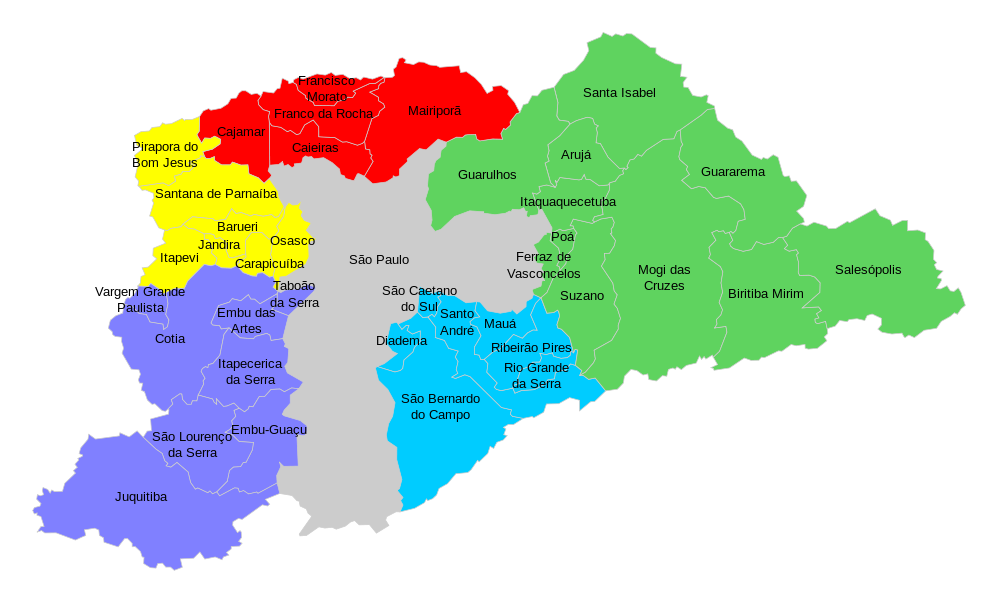
\includegraphics[width=0.9\textwidth]{./imagens/Mapa-RMSP-subregions.png}%
    \end{center}%
    \fonte{Mapa elaborado por Marcos Elias Oliveira Júnior, segundo a Lei 1.139/2011 \cite{LEI1139}. Disponível em: \url{http://pt.wikipedia.org/wiki/Regi\%C3\%A3o_Metropolitana_de_S\%C3\%A3o_Paulo\#mediaviewer/File:Mapa-RMSP-subregions.svg} Acesso em 10 de novembro de 2014}
\end{figure}%

\section{Gênero}
% META: 10p.

Ao nascer, umas das primeiras atividades do ser humano é comunicar-se, o que inclui nominar para si o mundo que o cerca. Esse processo não se dá de maneira solitária, a nominação advém de uma interação social que visa compartilhar signos afim de efetivar a comunicação. Por isso, este capítulo visa estabelecer o que se deseja exprimir através de palavras-chave deste trabalho (gênero, mobilidade e sustentabilidade), considerando a visão de Bakthin, cujo trabalho, segundo \citeauthoronline{STELLA2005} (\citeyear{STELLA2005}), indicava ser necessário

\begin{citacao}
não somente a palavra, mas também a linguagem em geral, ser concebida e tratada de uma outra forma, levando-se em conta sua história, sua historicidade, ou seja, especialmente a linguagem em uso. Isso significa que, no pensamento bakthiniano, a palavra reposiciona-se em relação às concepções tradicionais, passando a ser encarada como um elemento concreto de feitura lógica.
\end{citacao}

Há um senso comum que confunde e funde, não por acaso, os conceitos de sexo e gênero, muito embora sejam distintos - distinção esta encontrada em maior ou menor grau de acordo com o idioma. Em inglês a palavra \emph{sex} tem sentido mais limitado, ligado à anatomia, e a palavra \emph{gender} tem sentido mais amplo, ligado à construção cultural da identidade. Em francês, a palavra \emph{séxe} e, em alemão, a palavra \emph{Geschlecht}, designam tanto diferenças físicas como psicológicas, sociais e culturais \cite{FRAISSE2001}. \citeauthoronline{MORAES1998} (\citeyear{MORAES1998}) reporta que, em francês, frequentemente utiliza-se \emph{rapports sociaux de séxe} ao invés de \emph{gendre} para se designar \emph{gênero}. Comparado com o termo inglês \emph{gender}, ``a palavra gênero, em português, é um substantivo masculino que designa uma classe que se divide em outras, que são chamadas espécies'', definição então retirada do Novo Dicionário Aurélio por \citeauthoronline{MORAES1998} (\citeyear{MORAES1998}, p.101).
Já hoje, em 2014, o Dicionário \citeauthoronline{AURELIOONLINE} (\citeyear{AURELIOONLINE})
já comporta entre suas definições, aquela em que \emph{gênero} pode ser entendido como o ``conjunto de propriedades atribuídas social e culturalmente em relação ao sexo dos indivíduos''.
Porém, entre as definições mais gerais apresentadas pelo Dicionário \citeauthoronline{MICHAELISONLINE} (\citeyear{MICHAELISONLINE}), \emph{gênero} é definido da seguinte forma:

\begin{citacao}
s.m. (lat *\emph{generu}, por \emph{genus}) 1 Grupo de seres que têm iguais caracteres essenciais. 2 \emph{Lóg.} A classe que tem mais extensão e portanto menor compreensão que a espécie. 3 \emph{Biol.} Grupo morfológico intermediário entre a família e a espécie. 4 \emph{Gram.} Flexão pela qual se exprime o sexo real ou imaginário dos seres. 5 \emph{Gram.} Forma do adjetivo ou pronome com relação ao gênero dos nomes a que se refere. 6 Agrupamento de indivíduos que possuem caracteres comuns. 7 Espécie, casta, raça, variedade, sorte, categoria, estilo etc. 8 Qualidade, espécie, modo.
\end{citacao}

Percebe-se que o termo gênero designa um conceito em construção e consolidação, não apenas no Brasil, sendo necessário defini-lo sempre que o utilizarmos como denominação de categoria de análise \cite{MORAES1998}. Para isso, será feito um breve apanhado do surgimento e trajetória da palavra \emph{gender} ou \emph{gênero} nas pesquisas acadêmicas, inclusive no Brasil, bem como a evolução do conceito.

O conceito fundido e identitário de sexo e gênero, como se fossem sinônimos, pertenece a uma visão binária de mundo que define as mulheres mais próximas das natureza, do trabalho reprodutivo, da passividade e do irracional e, em oposição, define os homens mas próximos à cultura, ao trabalho produtivo, à ação e à racionalidade \cite{HARAWAY2004}.
Estudiosas feministas, rejeitando o determinismo bio-sexual para a situação social das mulheres, precisavam desmontar a naturalização das diferenças entre homens e mulheres que vinculava suas relações sociais, políticas e econômicas a seu aparelho reprodutor \cite{PISCITELLI2009}. 
Para \citeauthoronline{HARAWAY2004} (\citeyear{HARAWAY2004}, p.218), as feministas lutaram ``para remover as mulheres da categoria da natureza e colocá-las na cultura como sujeitos sociais na história, construídas e auto-construtoras''. Desssa forma, a evolução do conceito de gênero mescla-se à história do feminismo.

A chamada ``primeira onda feminista'' ocorreu entre o final do século XIX e o início do século XX nos países hoje considerados desenvolvidos da Europa e da América do Norte. A principal bandeira reivindicava direitos iguais, compondo uma ideia de que deveria haver uma igualdade entre os sexos. Em decorrência dessa primeira movimentação, em diversos países, as mulheres conquistaram alguns direitos equivalentes aos dos homens, como o voto. Essa conquista do voto como um direito político caracterizou o movimento sufragista, que não pode ser confundido com o movimento feminista, embora seja parte dele.
A Finlândia foi o primeiro país a garantir direito a votar e ser votado(a) igualmente a mulheres e homens, em 1906, quando ainda era um Principado do Império Russo \cite{RAY1918}.
Na Inglaterra, em 1865, John Stuart Mill apresenta ao Parlamento um projeto de lei dando o voto às mulheres, que não foi aprovado. Somente em 1928, o voto feminino é autorizado nas mesmas condições às dos homens \cite{NELSON2004}.
Nos Estados Unidos, foi em 1920 aprovada a 19ª Emenda
\footnote{Fonte: \url{http://www.archives.gov/historical-docs/document.html?doc=13&title.raw=19th+Amendment+to+the+U.S.+Constitution:+Women\%27s+Right+to+Vote} Acesso em 02 de novembro de 2014.} que proíbia o estabelecimento de qualquer restrição ao voto (estadual e federal) baseada no sexo do(a) votante. 
 
Na década de 1930, Mead, uma antropóloga estadunidense, problematiza a fixitude dos conceitos \emph{feminilidade} e \emph{masculinidade} a partir de uma pesquisa comparativa entre três sociedades tribais na Nova Guiné  \cite{MEAD2000}. A pesquisadora conclui não haver um temperamento inato, universal que tenha origem biológica, ligada ao aparelho reprodutor. Ela observa que traços de caráter são aprendidos em sociedade, podendo, portanto, ser modificados e até desaprendidos. Ela deixa legado teórico que suporta a ideia de que existe uma construção cultural da diferença sexual.
%http://pt.scribd.com/doc/178229042/Resumo-Sexo-e-Temperamento-Margareth-Mead

Em 1949, a filósofa francesa Beauvoir lança a obra \emph{O Segundo Sexo}, considerado precursor da ``segunda onda feminista''\cite{PISCITELLI2009}. Ainda que \citeauthoronline{BEAUVOIR1967} (\citeyear{BEAUVOIR1967}) não cite o conceito de  ``papel social'' ou mesmo ``papel sexual'', ela enfatiza logo de início que o ``ser uma mulher'' é uma construção social:

\begin{citacao}
nenhum destino biológico, psíquico, econômico define a forma que a fêmea humana assume no seio da sociedade; é o conjunto da civilização que elabora esse produto intermediário entre o macho e o castrado que qualificam de feminino.
\cite[p.09]{BEAUVOIR1967}
\end{citacao}

Em sua obra, \citeauthoronline{BEAUVOIR1967} (\citeyear{BEAUVOIR1967}) tem por foco questionar a dominação masculina, sem deixar de questionar também a eficácia do movimento feminista forjado até então no combate a essa dominação. Ela julgava ser possível esse combate ser bem sucedido se fossem combatidos elementos como: forma com que mulheres eram educadas; instituição de casamentos opressores; maternidade compulsória; vigência de um duplo padrão de moralidade sexual que permitiam maior liberade sexual somente aos homens; e falta de trabalhos dignos e bem remunerados que possibilitassem independência econômica às mulheres. 

Quase que concomitantemente, nos Estados Unidos, nasce um novo par de categorias de estudos, o sexo-gênero \cite{FRAISSE2001,STOLKE2004,HARAWAY2004}. A distinção entre as característica biológicas e as características sociais torna-se mais difundida, ou seja, na academia e na sociedade passa a ser considerada a noção de que posturas sociais de identidade masculina ou feminina não estabelecem relação biunívoca com o sexo anatômico.
A nominação dessa construção cultural pela palavra gênero ocorre em 1958, na Califórnia, quando foi empreendida uma pesquisa acerca da identidade de gênero no \emph{California Gender Identity Center}. Os resultados foram apresentados pelo psicanalista Robert Stoller em 1963, no Congresso de Pscicanálise de Estocolmo. Essa mesma pesquisa embasou a elaboração do primeiro volume de \emph{Sex and Gender} de \citeauthoronline{STOLLER1968} (\citeyear{STOLLER1968}). Essa obra expôs o quanto a relação sexo e gênero não é automática, nem estrita, discorrendo ainda sobre casos em que a anatomia da genitália não seria compatível com a identidade masculina ou feminina da pessoa. Assim, Stoller formula um conceito de gênero ligado à cultura, enquanto o conceito de sexo permanece ligado à morfologia corporal.

Em 1970 e 1980, o debate sobre esse par de categorias (sexo-gênero) toma espaço na comunidade acadêmica estadunidense. A antropóloga \citeauthoronline{RUBIN1975} (\citeyear{RUBIN1975})  introduz a categoria gênero no debate sobre opressões sociais sofridas pelas mulheres por meio do seu ensaio \emph{The Traffic in Women: Notes on the 'Political Economy' of Sex}. Nessa obra, \citeauthoronline{RUBIN1975} faz uma análise marxista sobreposta ao sistema sexo-gênero da qual depreende que no sistema de trocas capitalista, os homens estabelecem-se como vendedores e as mulheres são estabelecidas como mercadorias para serem trocadas.
Rubin dialoga com Lévi-Strauss que aponta ser o casamento o dispositivo mais importante de aliança entre as famílias, inexistente se não fosse pelo \emph{tabu do incesto} \cite{STRAUSS2010}. Para \apudonline{RUBIN1975}{PISCITELLI2009} esse tabu é precedido por outro, o da \emph{homossexualidade}. Isso porque, mediante a divisão sexual do trabalho
\footnote{A expressão \emph{divisão sexual do trabalho} foi inicialmente utilizada por etnólogos para se referir à repartição das atividades entre homens e mulheres nas sociedades que estudavam \cite{KERGOAT2004}. Esta autora afirma ainda que ``a divisão sexual do trabalho é aquela decorrente das relações sociais de sexo'', o que será explorado mais adiante neste capítulo.} e ao tomar como a menor unidade de sobrevivência econômica a família, tem-se necessariamente um homem e uma mulher, numa relação heterossexual de dependência mútua. Rubin discute também o trabalho doméstico, dando visibilidade a um trabalho que muitas vezes viabiliza o sustento do trabalhador (geralmente homem) sem que seja remunerada (a mulher). Por fim, ela consegue articular teoricamente gênero e sexualidade de forma que o conceito de gênero constituído até então não reside apenas em identificação com um determinado sexo, mas pressupõe que o desejo sexual seja por indivíduo do sexo oposto. 
% \url{https://ensaiosdegenero.wordpress.com/tag/gayle-rubin/} 
% \url{http://ensaiosdegenero.wordpress.com/2012/04/16/o-conceito-de-genero-por-gayle-rubin-o-sistema-sexogenero/}

A distinção entre sexo e gênero foi extremamente útil às feministas acadêmicas, pois sinalizava um lastro teórico para embasar os estudos sobre a condição da mulher, muitas vezes inferiorizada por sua condição biológica inerente. Com isso, o questionamento à lógica binária de interpretação do mundo passou a ser menos frequente e incisivo \cite[p.218]{HARAWAY2004} e, porque não, superada em alguma medida. Conforme pode-se ver no trabalho de Rubin, o conceito de gênero foi além de separar dimensões culturais e biológicas de mulheres e homens. Cada vez mais o conceito de gênero passa a significar também a superação da leitura binária de mundo que só permite feminilidade ou masculinidade. Para \citeauthoronline{HEILBORN1992} (\citeyear{HEILBORN1992}, p.41):

\begin{citacao}
A categoria de gênero não deve ser acionada como um substituto de referência para homem ou mulher. Seu uso designa, ou deveria fazê-lo, a dimensão inerente de uma escolha cultural e de conteúdo relacional. Por outro lado, traz embutida a articulação desse código, que se apropria da articulação da diferença sexual tematizando-a em masculino e feminino, com outros níveis de significação dos universos.
\end{citacao}

Se a primeira onda do feminismo reinvindicou direitos iguais, a segunda onda avançou e lutou pelo exercício igual dos direitos. Na primeira onda buscava-se provar que as diferenças entre o feminino e o masculino eram de origem social e não biológica. Tal afirmação não é abandonada na segunda onda, mas aprofundada, passando-se a buscar as origens de tais diferenças sócio-culturais. Nessa construção, segundo \citeauthoronline{PISCITELLI2009} (\citeyear{PISCITELLI2009}, p.133-134):

\begin{citacao}
A categoria ``mulher'' foi desenvolvida pelo feminismo da segunda onda em leituras segundo as quais a opressão das mulheres está além de questões de classe e raça, atingindo todas mulheres, inclusive as mulheres das classes altas e brancas. [...] O reconhecimento político das mulheres como coletividade ancora-se na ideia de que o que une as mulheres ultrapassa em muito as diferenças entre elas. Isso criava uma ``identidade'' entre elas.
\end{citacao}

Se essa uniformização entre as mulheres foi útil para forjar uma união na conquista por direitos, em meados da decada de 1970 e início dos anos 1980, já era questionada. Feministas negras e mulheres de países subdesenvolvidos \cite{FURTADO2009} cada vez menos identificavam-se com o arcabouço teórico hegemônico e homogêneo apresentado por feministas dos países do ``norte rico'', inclusive por Rubin. Assim, a ``terceira onda feminista'' desdobra-se em feminismos diversos. Afinal, as mulheres negras contam com trajetória histórica diferente das mulheres brancas, grande parte das vezes tendo a escravidão e suas consequências como parte determinante da vida de sua ancestralidade \cite{HOOKS1990,CRENSHAW2002}. No caso de países subdesenvolvidos, como o Brasil, não cabe comparar \emph{ipsis literis} a trajetória das mulheres (mesmo brancas) brasileiras com as europeias. A título de ilustração, o estudo de \citeauthoronline{PINTO2004} (\citeyear{PINTO2004}) apresenta como as mulheres brasileiras são vistas como mais maternais, com vocação para a domesticidade e muito mais ``racializadas'' do que as portuguesas.

%Mas, segundo \citeauthoronline{WIZEMAN2001}(\citeyearonline{WIZEMAN2001}) os termos sexo e gênero não são sinônimos e, conforme definição adotada pelo Instituto de Medicina da \emph{National Academy of Sciences} o sexo é uma classificação ``de acordo com os órgãos reprodutores e funções [biológicas] atribuídas pelo complemento cromossômico''. Gênero, por sua vez, é a ``auto-representação de um pessoa como masculino ou feminino, ou como a pessoa é percebida por instituições sociais com base na apresentação de gênero do indivíduo''.

Oferecendo alguma resposta a essas demandas por interseccionalidade
\footnote{Interseccionalidade, segundo \citeauthoronline{CRENSHAW2002} (\citeyear{CRENSHAW2002}, p.177) ``trata especificamente da forma pela qual o racismo, o patriarcalismo, a opressão de classe e outros sistemas discriminatórios criam desigualdades básicas que estruturam as posições relativas de mulheres, raças, etnias, classes e outras.''} em 1986, a historiadora pós-estruturalista Joan Scott publica seu artigo \emph{Gender: A Useful Category of Historical Analysis} em que faz uma leitura crítica da utilização do termo \emph{gênero} como categoria de análise e relaciona necessariamente esta categoria a outras como classe e raça, pois demonstra ser o gênero necessariamente imbricado a relações hierarquizadas de poder:

\begin{citacao}
a oposição binária e o processo social das relações de gênero tornam-se,
ambos, partes do sentido do próprio poder. Colocar em questão ou mudar um aspecto ameaça o sistema por inteiro. Se as significações de gênero e de poder se constróem reciprocamente, como é que as coisas mudam? [\ldots] o gênero tem que ser redefinido e reestruturado em conjunção com uma visão de igualdade política e social que inclui não só o sexo, mas também, a classe e a raça. \cite[p.1073,1075]{SCOTT1986}
\end{citacao}

%Assim como Scott, a filósofa estadunidense Judith Butler também tem influência foucaultiana e é pós-estruturalista. Em sua obra \emph{Gender Trouble: Feminism and the Subversion of Identity} publicada em 1990 Butler questiona a coerência entre sexo (biológico), gênero (construção cultural) e desejo (sexual). Para ela, existe uma regra tácita  heterossexual socialmente aceita como correta, estimulada, e que exige uma determinada coerência na tríade sexo-gênero-desejo. A partir dessa foram de ler o gênero, articulado ao desejo sexual, é que pessoas transgênero passam a ter algum arcabouço teórico que lhes abarque. \citeauthoronline{BUTLER1999} (\citeyear{BUTLER1999}) descreve a performatividade, logo, para ela, o gênero seria um ato intencional, performativo e que gera significados.

É então necessário olhar a construção das identidades de gênero à luz das relações de poder e olhar brevemente como se deu a evolução dos direitos, especialmente na sociedade brasileira. As mulheres no Brasil escravocrata dispunham de uma grande imobilidade geográfica e mesmo as mulheres das classes dominantes raramente saíam às ruas e, quando o faziam, nunca estavam desacompanhadas \cite{SAFFIOTI2013}. Mulheres e homens de então desfrutavam de maneira assimétrica do direito de ir e vir.

Na campo dos direitos políticos, o movimento sugfragista das brasileiras não teve tanta capilaridade nem foi um movimento de massas como nos Estados Unidos, Inglaterra ou Rússia. Ele teve início na década de 1910, quando o Partido Republicano Feminino é fundado no Rio de Janeiro com o objetivo de instaurar o debate acerca do voto feminino 
\footnote{
Bertha Lutz, filha do cientista Adolfo Lutz, licenciou-se em Ciências Naturais na Sorbonne de Paris e, ao retornar ao Brasil, funda a Federação Brasileira pelo Progresso Feminino, em 1919, que leva adiante a luta pelo sufrágio feminino \cite{PINSKY2003}. A primeira cidade a autorizar o voto feminino em eleições foi Mossoró (RN), em 1928. Em nível nacional, Getúlio Vargas autoriza em 1931 o voto feminino apenas às mulheres solteiras, viúvas com renda própria ou casadas com a autorização do marido.}.
A igualdade de condições de voto entre homens e mulheres se concretiza em 1932, pelo Decreto nº 21.076 que autoriza o voto a qualquer cidadã ou cidadão com idade superior a 21 anos. A eleição de 1933 foi a primeira em que mulheres puderam participar do pleito, votando e sendo votadas, como Carlota Pereira Queiroz, a primeira deputada brasileira, que participou da Assembleia Nacional Constituinte entre 1934 e 1935 \cite{TABAK1989}.

Embora o direito ao voto tenha sido emblemático, a ideia de desfrutar de \emph{direitos iguais} na sociedade, mulheres e homens, tratava também de outros direitos como o acesso à educação e poder ter posse de bens - por muito tempo, de acordo com a lei, só homens podiam ser proprietários de casas, por exemplo \cite{PISCITELLI2009}. Subjacente a esses questionamentos das mulheres tecia-se o conceito de ``papel social'', bastante difundido a partir da década de 1930. Para \citeauthoronline{PISCITELLI2009} (\citeyear{PISCITELLI2009}, p.127), a teoria dos papeis sociais buscava:

\begin{citacao}
compreender os fatores que influenciam o comportamento humano. A ideia é que os indivíduos ocupam posições na sociedade, desempenhando papeis de filho, de estudante, de avô. [...] A ideia de posições ocupadas no desempenho dos papeis faz referência a categorias de pessoas que são reconhecidas coletivamente. Um dos atributos que podem servir de base para a definição dessas categorias é a idade. [...] Outro desses atributos pode ser o sexo. Nesse caso, homens e mulheres desempenham papeis culturalmente construídos: os papeis sexuais.
\end{citacao}

Essa busca por um leque de direitos não foi um movimento só das mulheres, mas um movimento de luta por cidadania
\footnote{A cidadania, para \citeauthoronline{CARVALHO2002} (\citeyear{CARVALHO2002}), é entendida como o exercício pleno de três direitos: direitos civis, direitos sociais e direitos políticos. Os civis são aqueles considerados direitos fundamentais, como o direito à vida, à liberdade, à propriedade, à igualdade perante a lei. Eles garantem a vida em sociedade e dependem da existência de uma justiça independente, eficiente, barata e acessível a todos. Os políticos se referem à participação do cidadão no governo da sociedade. Seu exercício é limitado a uma parcela da população definida por idade, por exemplo, e consiste na capacidade de fazer demonstrações políticas, de organizar partidos, de votar, de ser votado. Por fim, os sociais são aqueles que garantem a participação na riqueza coletiva e se baseia na ideia de justiça social. Incluem os direitos à educação, ao trabalho, ao salário justo, à saúde, à aposentadoria.}. Sob o ponto de vista de gênero e cidadania, \citeauthoronline{BRITO2001} (\citeyear{BRITO2001}) relembra que o conceito clássico de cidadania, o grego, excluía mulheres e escravos. Ela pontua que ao longo da história as identidades de homens e mulheres foram construídas pressupondo uma dicotomia entre o âmbito público e o privado. \citeauthoronline{BLAY2001} (\citeyear{BLAY2001}) relata que até os anos 1960/1970 era um fator negativo para a mulher participar da vida pública.
A partir de 1970, com o movimento feminista passa a haver críticas e questionamentos quanto à natureza, à separação e à natural atribuição dessas esfera a um determinado sexo. Assim, elabora-se uma perspectiva de análise a partir do gênero, e não do sexo biológico, pois o conceito de gênero também compreende as dimensões social e política do termo.

A partir dos anos 1990 o uso da categoria gênero tornou-se mais frequentemente utilizada no Brasil e, cada vez mais influenciada pelas diversas escolas de psicanálise para explicar a produção e a reprodução da identidade de gênero do sujeito.
A psicanalista brasileira \citeauthoronline{KEHL1998} (\citeyear{KEHL1998}) embora não tenha como central esse debate, participa dele e em sua obra \emph{Deslocamentos do Feminino}, ao invés de apartar sexo de gênero, assinala que gênero é um conceito que inclui a dimensão biológica do sexo, não sem somar-lhe atributos que a cultura provê.
A partir de Scott é cada vez mais corrente incorporar a dimensão da política e do poder na composição do conceito de gênero, conforme explicita \citeauthoronline{MORAES1998} (\citeyear{MORAES1998}, p.100):

\begin{citacao}
A expressão relações de gênero, tal como vem sendo utilizada no campo das ciências sociais, designa, primordialmente, a perspectiva culturalista em que as categorias diferenciais de sexo não implicam o reconhecimento de uma essência masculina ou feminina, de caráter abstrato e universal, mas, diferentemente, apontam para a ordem cultural como modeladora de homens e mulheres. Em outra palavras, o que chamamos de homem e mulher não é o produto da sexualidade biológica, mas sim de relações sociais baseadas em distintas estruturas de poder.
\end{citacao}

Essas relações de poder incidem tanto sobre as relações que se desdobram no espaço público, quanto as do espaço privado. No espaço público, ou não-doméstico, tem relevância para o presente estudo o mercado de trabalho. Ao longo do tempo, a urbanização e a industrialização levaram à ampliação da classe média e ao crescimento do consumo no Brasil. As mulheres entraram também neste processo, embora a maior parte das trabalhadoras tenha sido absorvida, ao menos inicialmente, no setor de serviços e com enorme concentração nos empregos domésticos, de menor rendimento. Constata-se assim que existe aqui uma divisão sexual do trabalho \cite{KERGOAT2004}, que tem por características a destinação prioritária dos homens à esfera produtiva e das mulheres à esfera reprodutiva. Essa forma de divisão pauta-se em dois princípios: o da separação e o da hierarquização. O princípio da separação explicita a ideia de que há ``trabalhos de mulheres'' e ``trabalhos de homens'' enquanto o princípio da hierarquização indica existir uma diferença de valoração entre o trabalho do homem (produtivo, mais valioso) e o da mulher (reprodutivo, menos valioso). \citeauthoronline{BLAY2001} (\citeyear{BLAY2001}, p.84) fala sobre a mulher brasileira:

\begin{citacao}
Até a década de 1960 a história, quando focalizava a mulher, atinha-se às supostas atividades femininas fundamentais, isto é, às de um ser apêndice da família. A historiografia simplesmente ignorava a participação feminina no mercado de trabalho, a enorme freqüência com que sustentavam economicamente a si e aos seus.
\end{citacao}

Ao longo do século XX, observou-se aumento de mulheres na população economicamente ativa brasileira \footnote{A população economicamente ativa é obtida pela soma da população ocupada e desocupada com 16 anos ou mais de idade. ``População ocupada'' compreende as pessoas que, num determinado período de referência, trabalharam ou tinham trabalho mas não trabalharam (por exemplo, pessoas em férias). ``População desocupada'' compreende as pessoas que não tinham trabalho, num determinado período de referência, mas estavam dispostas a trabalhar, e que, para isso, tomaram alguma providência efetiva nos últimos 30 dias (consultando pessoas, jornais, etc.). Fonte: IBGE - disponível em \url{http://www.ibge.gov.br/apps/snig/v1/?loc=0,355030&cat=118,119,1,2,-2,-3&ind=87} Acesso em 21 de novembro de 2014} 
(ver Gráfico \ref{graf:evolucao-pea}). 
%e a maior frequência feminina em empregos de jornadas menores (ver Gráfico \ref{graf:percent-jornadas})
O fenômeno permanece no século XXI de acordo com estudo da \citeauthoronline{ABRAMO2010} (\citeyear{ABRAMO2010}):
(i) observa-se que de 2001 a 2010 manteve-se a preponderância feminina em ocupações que demandam de 20 a 40h semanais;
(ii) para homens, manteve-se o predomínio histórico de jornada superior a 40h semanais;
(iii) o ingresso das mulheres no mercado de trabalho não alterou drasticamente o papel delas na família e, portanto, nas atividades ligadas às tarefas domésticas. Isto é, apesar de muitas mulheres terem entrado no mercado de trabalho algumas décadas atrás, elas ainda são responsáveis pela maior parte do trabalho doméstico. No Gráfico \ref{graf:jornadas-completas} é possível constatar não apenas essa divisão sexual do trabalho - produtivo, no mercado, e reprodutivo, no lar - mas também que as jornadas totais que acabam ficando a cargo da mulher são maiores. Os homens acumulam uma jornada de cerca de 50 horas por semana, as mulheres, 57 horas semanais.

\begin{grafico}[htb]%
    \caption{\label{graf:evolucao-pea}Percentual de indivíduos economicamente ativos, por sexo, no Brasil, entre 1950 e 2010}%
    \begin{center}%
        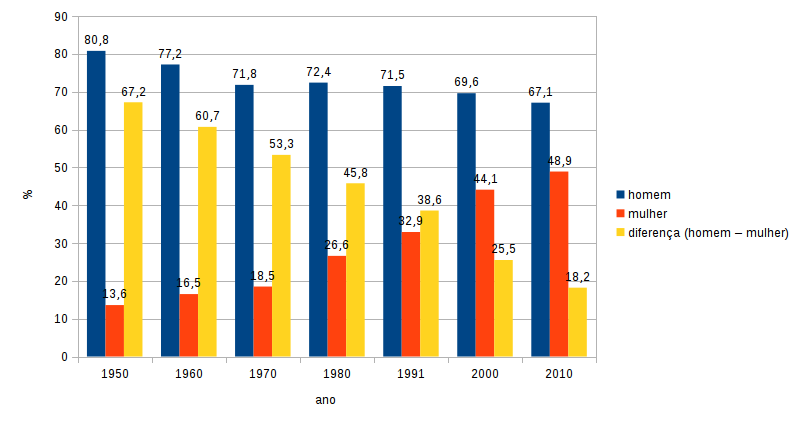
\includegraphics[width=1.05\textwidth]{./imagens/evolucao-pea1.png}%
    \end{center}%
    \fonte{Adaptado de \cite{ALVES2013}}
\end{grafico}%

%\begin{grafico}[htb]%
%    \caption{\label{graf:percent-jornadas}Percentual de trabalhadores(as) com jornadas de trabalho semanal acima de 44 horas e 48 horas e abaixo de 35 horas, por sexo, no Brasil, em 2008}%
%    \begin{center}%
%        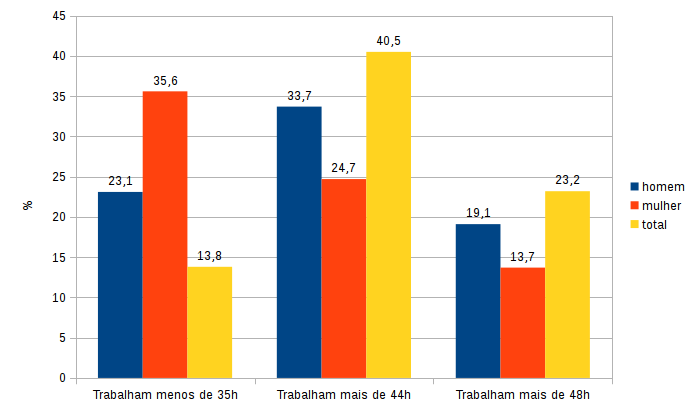
\includegraphics[width=0.9\textwidth]{./imagens/jornada-muler2003.png}%
%    \end{center}%
%    \fonte{\apud[p.01]{PNAD2008}{OIT2008}}
%\end{grafico}%

\begin{grafico}[htb]%
    \caption{\label{graf:jornadas-completas}Jornadas Médias para o Mercado de Trabalho e para Reprodução Social, por sexo, raça/cor e região geográfica, no Brasil, em 2003}%
    \begin{center}%
        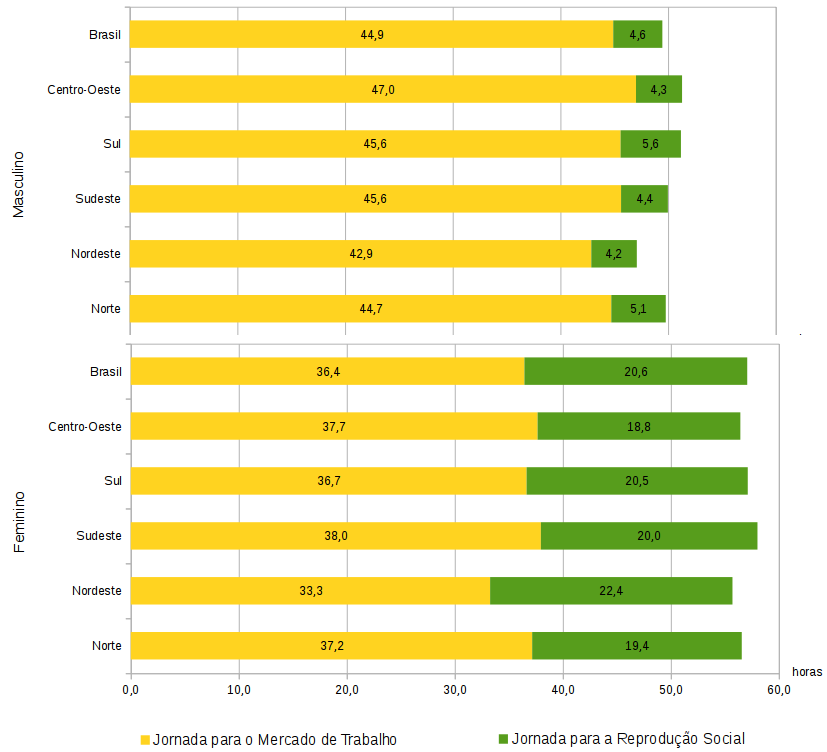
\includegraphics[width=0.9\textwidth]{./imagens/jornadas-totais.png}%
    \end{center}%
    \fonte{PNAD, 2003 apud \citeauthoronline{SOARES2003}, \citeyear{SOARES2003}}
    \nota{Segundo \citeauthoronline{DEAR1981} (\citeyear{DEAR1981}), o espaço de reprodução é onde a recuperação da força de trabalho ocorre sendo a residência o local principal a ser considerado; e o espaço de produção é onde o processo de acumulação do capital ocorre, ou seja, no que se denomina mercado de trabalho (indústria, comércio e serviços no geral).}
\end{grafico}%

%Mais um parágrafo sobre a divisão sexual do trabalho, dos papeis sociais - citar hirata aqui!

Esse é o ponto em que a atuação no espaço público e a no espaço privado vincula-se.
A mulher passa a poder desempenhar atividades antes tidas como ``masculinas'', porém sem ser desonerada de desempenhar as atividades tidas como ``femininas'', pois  ainda ``persistem nichos onde vigora uma imagem feminina vinculada à maternidade e ao cuidado da família, à saúde da prole'' \cite[p.94]{BLAY2001}. 
Assim, a ampliação do leque de papéis sociais que a mulher desempenha impacta as relações de poder dentro do ambiente doméstico, dentro da família. Isso molda as necessidades, interesses, atividades e padrão de viagens dos integrantes da família, a partir das identidades de gênero constituídas, forjadas pelos comportamentos de indivíduos e da relação de poder estabelecida entre eles.

\clearpage
\section{Mobilidade Urbana}
% META: 10p.

A palavra mobilidade, de acordo com o Dicionário \citeauthoronline{MICHAELIS2014},
significa ``(i) propriedade do que é móvel ou do que obedece às leis do movimento;
(ii) deslocamento de indivíduos, grupos ou elementos culturais no espaço social;
(iii) movimento comunicado por uma força qualquer;
(iv) falta de estabilidade, de firmeza ou inconstância''.
Tal definição reflete toda uma gama de conceitos relacionados a movimento e/ou deslocamento, o que na área de transportes relaciona-se imediatamente a viagens.
No Brasil, há cerca de 100 anos atrás a maior parte das viagens de pessoas era feita a pé
\footnote{Os primeiros carros foram montados em São Paulo pela Ford na década de 1910. Fonte: \url{http://www.carroantigo.com/portugues/conteudo/curio_hist_carro_brasileiro.htm} Acesso em 25 de outubro de 2014} 
e, quando muito, usava-se tração animal (cavalo ou boi), especialmente para cargas. Isso incorria em baixas velocidades de deslocamento e, assim, grande parte das pessoas acabavam por desenvolver suas atividades nas proximidades de onde nasceram por toda a vida. Nesses últimos dois séculos o cenário mudou bastante, as mais diversas tecnologias se desenvolveram, os rendimentos aumentaram, a mobilidade aumentou \cite[p.06]{METZ2012}, e como exemplos icônicos dessa maior mobilidade figuram a utilização do carro e do avião.

O conceito de mobilidade pode englobar muitos outros e se desdobrar em grande diversidade de temas.
Há quem o aborde ligando-o ao turismo \cite{ENLOE1989,FROHLICK2008}, enquanto outros \cite{CHANT1992,SILVEY2000} abordam-no sob a perspectiva dos movimentos migratórios entre países ou dentro de uma mesma nação. Outro uso do termo é ligado ao intercâmbio de estudantes e pesquisadores de diferentes instituições de origem – o que dá origem à expressão \emph{mobilidade acadêmica} \cite{ENDERS1998,TREMBLAY2005,HOFFMAN2008} . Ademais, há um olhar sobre a mobilidade em que as condições geo-demográficas são elementos de contorno, delimitando assim as áreas da mobilidade rural e urbana.
 
Embora pareçam óbvias à primeira vista – porque em alguma medida vividas – as diferenças entre rural e urbano são bem menos claras quando olhadas mais de perto. No Brasil as distinções nascem de critérios político-administrativos, originados em decreto de 1938
\footnote{Decreto-Lei nº 311, de 2 de Março de 1938 disponível em: \url{http://www2.camara.leg.br/legin/fed/declei/1930-1939/decreto-lei-311-2-marco-1938-351501-publicacaooriginal-1-pe.html} Acesso em 06 de novembro de 2014}
de Getúlio Vargas e, até hoje, no Brasil, baseia-se em critérios políticos administrativos. Segundo o IBGE, ``como situação urbana consideram-se as áreas correspondentes às cidades (sedes municipais), às vilas (sedes distritais) ou às áreas urbanas isoladas''
\footnote{Conceitos adotados no censo do IBGE disponíveis em: \url{http://www.ibge.gov.br/home/estatistica/populacao/contagem/conceitos.shtm}}. Como rural, classifica-se tudo o que não se configure urbano. Trata-se de definição legal (jurídica) ocorrida frequentemente no campo da política e passível de críticas, como a de \cite{GRABOIS2001} que aponta que tal classificação não considera as diferentes funções dos aglomerados como critério. A questão da definição do que é rural vai além da abordagem teórica e tem como pano de fundo as diferenças de tributação entre as áreas rural e urbana. Como saída a essa arbitrariedade que fica a cargo dos poderes municipais, \cite{VEIGA2002} elenca três critérios que entende importantes a se considerar nesse tipo de classificação: (i) população total do município, (ii) densidade demográfica e (iii) localização.

O objeto deste trabalho é a RMSP, composta por 39 municípios
\footnote{Os 39 municípios que compõem a RMSP são agrupados em 6 regiões de acordo com Lei Complementar estadual nº 1.139, de 16 de junho de 2011. Na região central está São Paulo. Na região Sudoeste encontram-se 8 municípios, a saber, Juquitiba, São Lourenço da Serra, Embu-Guaçu, Itapecerica da Serra, Embu, Tabão da Serra, Cotia e Vargem Grande Paulista. Na Região Oeste encontram-se 7 municípios, a saber, Pirapora do Bom Jesus, Santa de Parnaíba, Barueri, Jandira, Itapevi, Carapicuiba, Osasco. Na região Norte encontram-se 5 municípios, a saber, Cajamar, Caieira, Franco da Rocha, Francisco Morato, Mairiporã. Na região Leste encontram-se 11 municípios, a saber, Santa Isabel, Arujá, Guarulhos, Itaquaqueceteuba, Guararema, Poá, Suzano, Ferraz de Vasconcelos, Mogi das Cruzes, Biritiba Mirim, Salesópolis. Na região Sudeste encontram-se 7 municípios, a saber, Santo André, São Bernardo do Campo, São Caetano do Sul, Diadema, Mauá, Ribeirão Pires, Rio Grande da Serra.}; todos, atualmente, contam com áreas consideradas urbanas. 
Muito embora se vá seguir as classificações oficiais do IBGE e do Metrô-SP, entende-se como salutar esta breve discussão sobre o significado do que é ser área urbana ou rural, pois ``o espaço rural tem passado recentemente por um conjunto de mudanças com significativo impacto sobre suas funções e conteúdo social'' \cite[p.96]{MARQUES2002}. Deixa-se a ressalva de que mesmo na área de enfoque, urbana, encontram-se atividades agrícolas (comumente tidas como rurais), afinal, são cada vez mais imprecisos os limites entre um e outro \cite{MINGIONE1987}. Um outro fenômeno que merece alguma atenção, dada a natureza deste trabalho, é o êxodo rural seletivo que vem sendo constatado por alguns pesquisadores. \cite{RAUBER2010} constata no Rio Grande do Sul que a emigração do campo é desigual em gênero e em idade: mulheres e jovens migram mais, homens e idosos são os que permanecem no campo, nas atividades rurais. Fenômeno semelhante é constatado em Santa Catarina
\footnote{Êxodo seletivo é retratado em Santa Catarina pelo documentário ``Celibato no Campo'' de Cassemiro Vitorino e Ilka Goldschmidt, 2013, disponível em \url{http://www2.camara.leg.br/camaranoticias/tv/materias/OLHARES/440520-CELIBATO-NO-CAMPO.html} Acesso em 15 de outubro de 2014.},
e em alguns países europeus
\footnote{Relatório do Parlamento Europeu em 2003 apontava que somente 37\% da mão-de-obra rural da União Europeia era de mulheres. Disponível em \url{http://www.europarl.europa.eu/sides/getDoc.do?type=REPORT&reference=A5-2003-0230&format=XML&language=PT} Acesso em  16 de outubro de 2014}. Ou seja, existe diferença relacional entre a mobilidade feminina e a masculina expressa, por exemplo, nos deslocamentos campo-cidade.
O recorte deste trabalho, entretanto, concentra-se majoritariamente nos deslocamentos intra-urbanos, expressos amplamente pelo conceito de mobilidade urbana. 

Se ``o estudo dos problemas urbanos é indissociável da relação campo-cidade'' \cite[p.154]{FREITAG2007} e por isso, independente da época estudada, é preciso tê-la em mente; especificamente a mobilidade urbana é um elemento fundamental para que seja possível garantir aos habitantes de uma cidade acesso aos bens que lhes oferece \cite{IEMA2010}. Cabe aqui diferenciar o que seja mobilidade do que seja acessibilidade. A mobilidade exprime a capacidade de se delocar no espaço, ``refere-se à habilidade de mover-se entre dois diferentes locais de atividade'' \cite[p.04]{HANSON1995a}.
Sobre a acessibilidade e sua ligação com a mobilidade, \citeauthoronline{HANSON1995a} afirma ainda:

\begin{citacao}
A acessibilidade refere-se ao número de oportunidades [\ldots] disponíveis dentro de uma determinada distância ou tempo de viagem. [\ldots] Conforme as distâncias entre os locais de atividades se tornam maiores [\ldots] a acessibilidade passa a depender cada vez mais da mobilidade, particularmente daquela relacionada aos veículos particulares. \cite[p.04]{HANSON1995a}
\end{citacao}

Dessa maneira, vinculando a mobilidade à motorização, \citeauthoronline{HANSON1995a} afirma que é possível promover acessibilidade sem incrementar a mobilidade (1995, p.05), afinal, ter toda uma sorte de seviços próximos à residência daria a possibilidade de ir à padaria, ao mercado, à igreja, à escola, à livraria, etc. a pé. A autora ainda se aprofunda na questão da acessibilidade ao classificá-la como (i) de pessoas ou (ii) de lugares. Trata-se apenas de diferentes referenciais, a acessibilidade de uma pessoa indica o quão fácil ou difícil é para ela chegar a determinado local; a acessibilidade de um lugar mostra o quão fácil ou difícil pode ser alcançá-lo. Essas expressões ``fácil'' e ``difícil'', entretanto, são formas muita genéricas para caracaterizar o que se deseja exprimir. Problema para o qual ela apresenta como resposta uma medida de acessibilidade $A_{i}$ considerando $O_{i}$ oportunidades para a pessoa \emph{i}, distribuídas a distâncias \emph{j} da residência de \emph{i}:

\begin{equation}\label{eq:acessibilidade}
A_{i} = \sum_{i}^{} O_{i} d_{i,j}^ {-b}
\end{equation}

Caso considere-se ao invés de \emph{i} indivíduos, \emph{i} zonas, a Equação \ref{eq:acessibilidade} referir-se-á à zona \emph{i} de análise. Como este é um modelo bastante simplificado, indica apena um potencial de acessibilidade e tem suas limitações, como por exemplo, desconsiderando a dimensão temporal dos deslocamentos.
\citeauthoronline{VASCONCELLOS2012} (\citeyear{VASCONCELLOS2012}), por sua vez, pontua a questão temporal em sua definição de acessibilidade:

\begin{citacao}
medida pela quantidade e/ou diversidade de destinos que a pessoa consegue alcançar, por certa forma de transporte, em determinado tempo. Quanto maior for esta quantidade, maior é a acessibilidade, ou seja, mais oportunidades as pessoas terão para realizar atividades desejadas ou necessárias. \cite[p.42]{VASCONCELLOS2012}
\end{citacao}

O mesmo autor, em obra anterior, indica como forma de mensurar a acessibilidade, a soma dos tempos: (i) de deslocamento até o meio de transporte; (ii) tempo de espera, caso exista; (iii) tempos(s) dentro do(s) meio(s) de transporte; (iv) tempo de transferência entre diferentes meios de transportes, caso exista; (v) tempo após saída do meio de transporte até atingir o destino final. Destes tempos, ele classifica os itens (i) e (v) como \textbf{microacessibilidade}, ou seja, itens que referem-se ``à facilidade relativa de ter acesso aos veículos ou destinos desejados (por exemplo, condições de estacionamento ou acesso ao ponto de ônibus)'' (\citeyear{VASCONCELLOS2001}, p.91). A \textbf{macroacessibilidade} é definida por ele como a:

\begin{citacao}
facilidade relativa de atravessar o espaço e atingir construções e equipamentos urbanos desejados. Ela refelte a variedade de destinos que podem ser alcançados e, consequentemente, o arco de possbilidades de relações sociais, econômicas, políticas e culturais, dos habitantes do local. \cite[p.91]{VASCONCELLOS2001}
\end{citacao}

Isto posto, a acessibilidade pode ser entendida como a capacidade de se chegar onde se deseja e, para sua mensuração pode-se usar a distância e/ou o tempo. Uma das formas de reunir essas duas dimensões é através do prisma espaço-tempo. Na Figura \ref{fig:prisma} pode-se observar o diagrama do tempo em função da distância\footnote{Para ser um prisma, tal gráfico deveria ser em três dimensões: na base x e y representariam os deslocamentos no plano, e na altura, z, teríamos o tempo.} de um casal hipotético com filhos pequenos e um carro na família. Supondo que ambos trabalhem das 8h às 18h, que seja a mulher a levar as crianças na escola, a pé, e o homem a ficar com o carro da família, teríamos:

\begin{figure}[htb]%
    \caption{\label{fig:prisma}Prisma Espaço Tempo \hl{XXX} }%
    \begin{center}%
        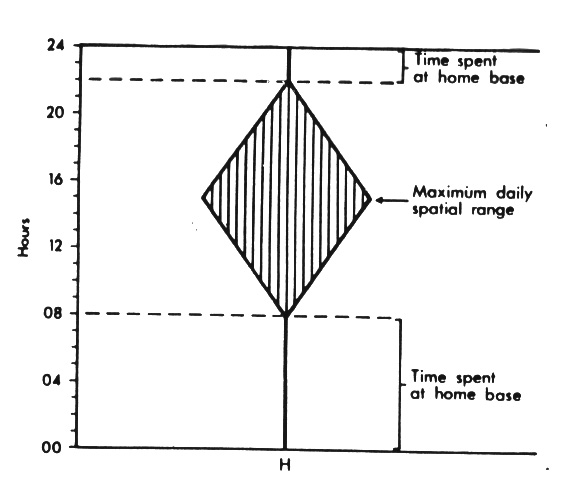
\includegraphics[width=0.75\textwidth]{./imagens/timeprism.jpg}%
    \end{center}%
    \fonte{Elaboração própria}
\end{figure}%
%http://www.anpet.org.br/xxviiianpet/anais/documents/AC301.pdf
%http://www.cetsp.com.br/sobre-a-cet/relatorios-corporativos.aspx

A situação narrada é hipotética, mas é ilustrativa de alguns fatores que restringem as liberdades de movimento, segundo \apud{HAGERSTRAND1970}{HANSON1995a}:
\begin{compactitem}
\item (i) limitações devido ao fato que não se pode estar em dois lugares ao mesmo tempo e que certas tarefas precisam ser feitas usando um determinado modo de transporte (por algum motivo pode não haver outras opções);
\item (ii) necessidade de encaixar os compromissos de uma pessoa com os de outra(s) pessoa(s), como por exemplo, levar filho(a)(s) à escola, acompanhar idoso(a)(s) ao médico ou almoçar com amigo(a)(s);
\item (iii) restrições devido à autoridade social, política e/ou legal no acesso a algum lugar - pode haver regras explícitas (ou implícitas), por exemplo, que impeçam as pessoas de andarem à noite sozinhas num determinado local.
\end{compactitem}

Só que as pessoas geralmente não dispõem de várias alternativas modais ou porque não têm recursos (ou para ter um carro ou para morar em área bem servida de transporte público) ou porque se sentem inseguras utilizando algum modo específico (medo de ser assaltado(a) no carro, de ser atropelado(a) de bicicleta, de ser assediada(a) no transporte público, entre outros). Não são todos(as) que podem arranjar horários flexíveis de trabalho e/ou de estudos para conciliar as outras atividades da forma mais eficiente, por exemplo, evitando os deslocamentos nos horários de pico. Enfim, as restrições incidem diferentemente nos grupos sociais criando assimetrias no acesso às oportunidades. Essa inequidade desdobra-se no espaço: na distribuição desigual de empregos nas cidades, na variação de preço do solo urbano, na densidade heterogênea de serviços públicos oferecidos nos diversos bairros e mesmo na ocupação do espaço de circulação (ver Figura \ref{fig:equidade}).

\begin{figure}[htb]%
    \caption{\label{fig:equidade}Quantidade de espaço viário requerido para transportar 60 pessoas por ônibus, bicicleta e carro.}%
    \begin{center}%
        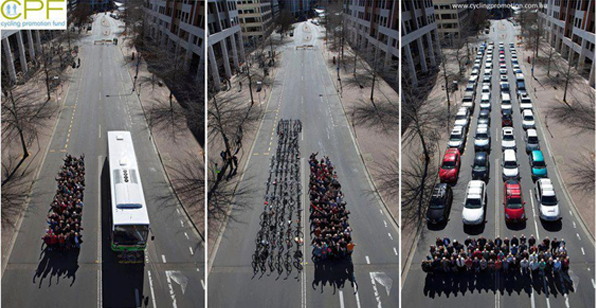
\includegraphics[width=0.75\textwidth]{./imagens/equidade-sqn.png}%
    \end{center}%
    \fonte{Foto de \emph{Cycling Promotion Fund}, disponível em \url{http://www.bhtrans.pbh.gov.br/portal/
page/portal/portalpublico/Temas/ObservatorioMobilidade/FiquePorDentro/ObsMobBH\%20A\%
20cidade\%20com\%20menos\%20carros} - acesso em 22 de novembro de 2014.}
\end{figure}%

Em 1991, 20\% da população de menor renda perfazia 9\% das milhas viajadas nos Estados Unidos (por carro e ônibus), ao passo que 20\% da população de maior renda concentrava 32\% \apud{CAMERON1994}{HANSON1995a}.
\citeauthoronline{VASCONCELLOS2001} (\citeyear{VASCONCELLOS2001}) apresenta o consumo de espaço, por modo de transporte e renda da RMSP em 1987 e 1997 (ver Tabela \ref{tab:consumoespaco}). Observa-se que na RMSP os grupos de maior renda tendem a consumir mais espaço de circulação, o que levanta a questão do quão (in)justo é esse cenário, principalmente no Brasil, onde o sistema de tributação que custeia a infra-estrutura pública urbana é regressivo
\footnote{O Brasil conta com um sistema de tributação regressivo, ou seja, aquele em que a retirada é proporcionalmente maior das pessoas com menor capacidade de contribuir \cite{GRECO2005}.}.

\begin{table}[htb]
    \IBGEtab{%\renewcommand{\arraystretch}{1.5}%%\ABNTEXfontereduzida%
	    \renewcommand{\arraystretch}{1.5}
        \caption{Consumo dinâmico de espaço por modo e renda na RMSP}
		\label{tab:consumoespaco}
    }{%
	    \begin{tabular}{P{3.50cm} P{3.5cm} P{3.5cm} P{3.5cm}}
            \toprule
	           \headerCell{Renda familiar mensal (1987)} &
		       \headerCell{Espaço dinâmico (km*$m^2$/dia/pessoa) (1987)} &
   	           \headerCell{Renda familiar mensal (1997)} &
		       \headerCell{Espaço dinâmico (km*$m^2$/dia/pessoa) (1997)}
	           \\
		    \midrule \midrule
		        0 a 240&
		        7,6&
		        0 a 250&		        
		        9,2\\
		    \midrule
		        241 a 480&
		        13,4&
		        251 a 500&		        
		        14,6\\
		    \midrule
		        481 a 900&
		        25,1&
		        501 a 1000&		        
		        23,7\\
		    \midrule
		        901 a 1800&
		        42,2&
		        1001 a 1800&		        
		        36,7\\
		    \midrule
		        1801 ou mais&
		        74,8&
		        de 1801 a 3600&		        
		        56,2\\		        
		    \midrule
		        -&
		        -&
		        3601 ou mais&		        
		        81,9\\		        
		    \bottomrule
		\end{tabular}
    }{%
		\fonte{Adaptado de \cite[p.181;196]{VASCONCELLOS2001}}
		\nota{Considerando consumo médio de $1,0m^2/pessoa$ em transporte público ($30m^2$ de área de ônibus para 30 passageiros em média) e $6,6m^2/pessoa$ em transporte privado ($10m^2$ de área de carro para 1,5 passageiros em média).}		
		}
\end{table}

%Portanto, a mobilidade é condição necessária mas não suficiente para a garantia da acessibilidade.
%A acessibilidade é o que liga a mobilidade urbana à equidade social.

Segundo \apudonline{URRY2004}{UTENG2008}, tendo em vista as inequidades urbanas de acesso, estruturadas socialmente, há cinco ``mobilidades'' bastante interdependentes:
\begin{compactitem}[]
\item (i) viagem corpórea das pessoas por motivo de trabalho, lazer, etc.;
\item (ii) movimento físico de objetos (cargas);
\item (iii) viagem imaginativa a lugares por meio de imagens (fotos ou televisão);
\item (iv) viagem virtual mediante uso da internet; 
\item (v) viagem comunicativa através de mensagens trocadas entre pessoas (cartas, mensagens de celular, telefone).
\end{compactitem}

\clearpage
Não é possível considerar então a mobilidade do indivíduo, isolando-o do seu contexto socia, econômico, político e cultural; muito pelo contrário, só é possível entendê-lo se considerarmos os ambientes em que se ancora: doméstico, familiar e social \cite{HANSON2010}. Por fim, cabe esclarecer que este trabalho adota para si os conceitos de micro e macroacessibilidade \citeauthoronline{VASCONCELLOS2001} (\citeyear{VASCONCELLOS2001}). Ademais, acrescido do significado de urbano definido pelo IBGE, trabalha com o conceito de mobilidade relacionado ao item (i) de \apudonline{URRY2004}{UTENG2008}, mais detalhado no artigo \emph{Gender and mobility: new approaches for informing sustainability} de \citeauthoronline{HANSON2010}, que emprega o termo \textbf{mobilidade} para designar:

\begin{citacao}
o movimento de pessoas de um lugar para outro lugar no decorrer da vida cotidiana [\ldots] [sendo a] principal preocupação com as viagens pessoais que compõem a rotina diária de atividades como o trabalho (remunerado e não remunerado), lazer, socialização e compras.
\cite[p.7]{HANSON2010}
\end{citacao} 


\clearpage
\section{Sustentabilidades}
% META: 10p.

Por definição de sustentabilidade encontram-se nos dicionários descrições bastante simples e amplas, que podem ser resumidas como ``a qualidade de ser sustentável'' \cite{MICHAELIS2014}, o que posterga a dúvida para a questão: o que é ser sustentável? Segundo \citeauthoronline{BLACK2010} (\citeyear{BLACK2010}), é aquilo que pode ser mantido ou que dure. É evidente que tal durabilidade não é eterna, mas por um determinado período. A ideia da permanência leva a crer que tal período seja longo, que relacione-se à perspectiva de longo prazo, mas de quão longo se trata, é uma indefinição, até hoje. Hoje, inclusive, é cada vez mais frequente o uso do termo sustentável como modificador ao invés de sustentabilidade como um conceito fechado em si. Aqui, exploraremos o desenvolvimento  sustentável e o transporte sustentável como as ``sustentabilidades'' de interesse.

As primeiras preocupações e dicotomizações entre desenvolvimento e meio ambiente remontam o fim da década de 1960, com o Clube de Roma
\footnote{O Clube de Roma fora fundado em 1968 por Aurelio Peccei e Alexander King e que consistia num grupo de pessoas ilustres (empresários, líderes religiosos, políticos, entre outros) que se reuniam para discutir assuntos ligados à política, economia e, também, meio ambiente. Para saber mais: \url{http://www.clubofrome.org/} Acesso em 06 de novembro de 2014.}, que será o berço da obra \emph{The Limits to Growth}. Este livro, publicado em 1972, problematiza pela primeira vez a questão do crescimento exponencial \emph{versus} a finitude dos recursos disponíveis e também se propõe a simular e tentar prever as consequências da intereção antrópica com sistemas não-antrópicos \cite{MEADOWS1972}. Nesse mesmo ano, ocorre a Conferência sobre o Ambiente Humano das Nações Unidas em Estocolmo.

Em 1983, as Nações Unidas (ONU) fundam a Comissão Mundial sobre Meio Ambiente e Desenvolvimento (WCED), composta por 19 delegados de 18 países, com a missão de produzirem um estudo sobre desenvolvimento em escala global, considerando aspectos como sustentabilidade e meio ambiente num perspectiva de longo prazo. Assim, a expressão ``desenvolvimento sustentável'' aparece pela primeira vez em \citeyear{WCED1987}, no relatório \emph{Our Common Future} da WCED, também conhecido como \emph{Brundtland Report} 
\footnote{Gro Harlem Brundtland era o Primeiro Ministro da Noruega e foi quem comandou a Comissão Mundial sobre Meio Ambiente e Desenvolvimento (WCED). Fonte: \url{http://www.un-documents.net/our-common-future.pdf} Acesso em 06 de novembro de 2014.}, onde é apresentado o clássico conceito:

\begin{citacao}
desenvolvimento sustentável é aquele que satisfaz as necessidades do presente sem comprometer a capacidade das gerações futuras satisfazerem as suas próprias necessidades. Este conceito contém em si outros dois conceitos-chave: o de ``necessidades'', em particular as necessidades essenciais dos pobres do mundo, às quais deve ser dada prioridade absoluta; e a ideia de limitações impostas pelo estágio tecnologico e de organização social sobre a capacidade do meio ambiente de satisfazer as necessidades presentes e futuras. 
\cite[p.41]{WCED1987}
\end{citacao}   

Essa definição consolidou-se na Conferência das Nações Unidas sobre Meio Ambiente e Desenvolvimento ocorrida em 1992 no Rio de Janeiro, também conhecida como ECO-92. Em quase vinte anos, o conceito popularizou-se, ganhou robustez e também ficaram mais nítidas suas limitações de implementação. Um relatório de balanço da ONU publicado em 2010 \cite{ONU2010} indica haver convergência conceitual de que o desenvolvimento sustentável está alicerçado sobre três pilares: desenvolvimento econômico, equidade social e proteção ambiental. O mesmo documento reconhece, porém, que apesar de visionário e integrador, o conceito tem se mostrado de difícil implementação pelos países e pouco tem sido abraçado em sua completude pelas políticas das diversas nações. 

Embora o desenvolvimento sustentável pretenda englobar os três pilares, o desenvolvimento é frequentemente sinônimo de desenvolvimento econômico e a sustentabilidade fica muitas vezes compartimentada à questão ambiental \cite{ONU2010}. Um dos caminhos que vem sendo cosntruído para tentar superaressa dificuldade é tornar o conceito menos difuso e mais palpável por meio de indicadores \cite{CHAMBERS2000,BOULANGER2008,BARRETT2010,FORTES2012} e metas (de preferência quantitativas) a serem atingidas num determinado prazo \cite{ONU2010,ONU2014}.

Outra saída, não excludente com esta recém apresentada, é adicionar outros pilares na conceituação do que seja desenvolvimento sustentável, como faz 
\citeauthoronline{BANISTER2005} (\citeyear{BANISTER2005}). Ele elenca outros dois fatores como fundamentais: (i) participação e (ii) governança. A dimensão da participação refere-se a envolver todas pessoas interessadas e envolvidas no processo, a saber, indivíduos, empresas, indústrias e governos. Argumenta que criar excluídos do processo torna muito mais difícil desenvolver as estratégias necessária de mudança. A dimensão da governança incide diretamente no processo de tomada de decisão, logo, significa mudanças nas estruturas organizacionais para que sejam facilitadas decisões intersetoriais.

\citeauthoronline{BANISTER2005} (\citeyear{BANISTER2005}) destaca cinco lições aprendidas desde o \emph{Brundtland Report} a partir das experiências de sucessos e fracassos: (i) as reduções devem começar modestamente; (ii) desestímulo às emissões de dióxido de carbono (CO$_2$) deve contar com mecanismos fiscais; (iii) deve haver incentivos fortes em pesquisa e desenvolvimento em ciência e tecnologia na temática das mudanças climáticas; (iv) embora todos países devam contribuir para a diminuição de emissões de carbono, a liderança cabe às nações mais ricas; (v) é preciso ação imediata e incerteza não é uma boa razão para inação ou atitudes fracas.
Ao se falar em sustentabilidades, fala-se necessariamente de mudanças de paradigma, profundas, e que podem até mesmo ser inatingíveis \cite{GLASBY2002}, embora possam ser perseguidas. \citeauthoronline{ROGERS2000} (\citeyear{ROGERS2000}) aponta que essa mudança deve necessariamente compreender as ``relações entre cidadãos, serviços, políticas de transporte e geração de energia, bem como seu impacto total no meio ambiente local e numa esfera geográfica mais ampla'' e aponta ainda as cidades, pensadas como organismos vivos, cujo metabolismo é bastante linear, precisando tornar-se mais circular (ver figura \ref{fig:cidade-metabolismos}).

\begin{figure}[htb]%
    \caption{\label{fig:cidade-metabolismos}Cidades de metabolismo linear e circular}%
    \begin{center}%
        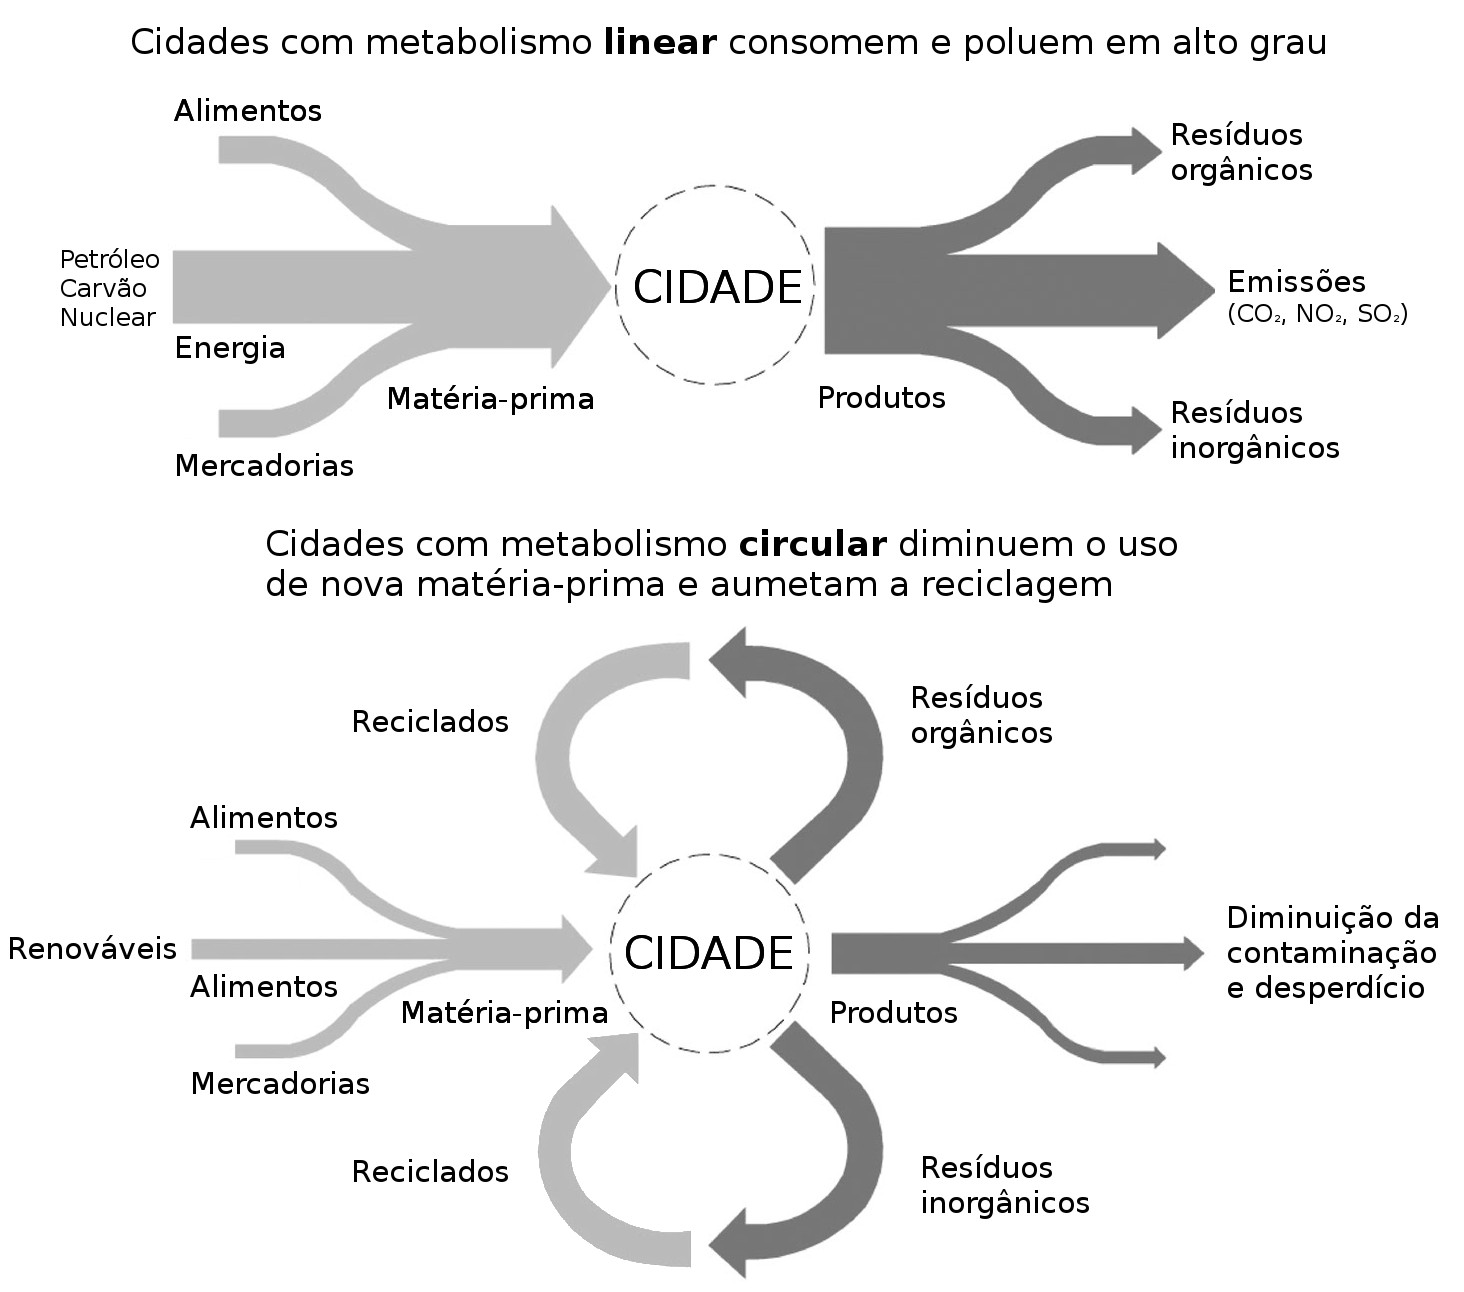
\includegraphics[width=0.80\textwidth]{./imagens/richard-linear-circular.jpg}%
    \end{center}%
    \fonte{\cite[p.31]{ROGERS2000}}
\end{figure}%

Do ponto de vista econômico, a obra \emph{Limits to Growth} fez escola e trouxe à baila a hipótese de que o crescimento econômico teria um teto, função dos recursos (naturais) disponíveis. Contudo, há estudiosos que se opõem a isso, como \citeauthoronline{KRUGMAN2014} (\citeyear{KRUGMAN2014}) em seu recente artigo \emph{Slow Steaming and the Supposed Limits to Growth}. O economista argumenta que é possível manter o crescimento econômico real (do PIB) e ainda assim reduzir a emissão de gases do efeito estufa. Para chegar a essa conclusão ele apresenta uma demonstração - bastante simplista - que considera o consumo de energia dos navios em função de suas velocidades e conclui ser possível manter um caudal econômico constante e, concomitantemente, diminuir o consumo de energia do sistema.

Entre as principais preocupações no âmbito ambiental estão a diminuição das reservas de petróleo, aquecimento global por conta da emissão de gases do efeito estufa, poluição (atmosférica, sonora e hídrica) e presença de chuva ácida. Diversos estudos indicam que exite correlação entre a ocorrência de diversos tipos de doenças (cardiorrespiratórias, câncer, entre outras) e a exposição alguns poluentes presentes na atmosfera \cite{WHO2000,WHO2006,BRUNEKREEF2012,MIRANDA2012}. Em São Paulo, \citeauthoronline{GOUVEIA2006} (\citeyear{GOUVEIA2006}) observaram associação estatisticamente significante entre o aumento no nível de poluentes na atmosfera e o aumento de hospitalizações por causas diversas, em todos grupos etários estudados. As emissões de CO$_2$, indicado como o principal gás responsável pelo efeito estufa, aumentaram cerca de 60\% e a parcela cuja origem são os sistemas de transporte também aumentou de 19,3\% para 28,9\% entre 1971 e 2001 \cite{BANISTER2005}.

Sob o prisma da equidade social, o acesso equânime a oportunidades de educação, trabalho, saúde e lazer é um dos pontos centrais. A equidade, associada à ideia do ``ser justo'', inevitavelmente referir-se-á à distribuição social de custos e benefícios , bem como em que grau essa distribuição é considerada adequada e que corrobore para a promoção da justiça \cite{LITMAN2006}. Aqui também o transporte tem papel estruturador já que pode ser o elemento que provê ou barra o acesso às oportunidades. \citeauthoronline{SANCHEZ2003} (\citeyear{SANCHEZ2003}) já apontava que equidade seria um dos temas estratégicos nas políticas de transportes. As megalópoles latino-americanas são, por vezes, cidades ``partidas'' \cite{VENTURA2001} entre a ``legal'' e a ``real'' \cite{ALVA1997}
\footnote{Estima-se que cerca de 40\% ou mais da população possui moradia em condição irregular \cite{FREITAG2007}.},
onde as vias de circulação frequentemente são cicatrizes no tecido urbano - por exemplo, em São Paulo, o ``Minhocão'' \cite{ABASCAL2010}, os monotrilhos \cite{ROLNIK2010} ou mesmo uma rua na favela de Paraisópolis (ver Figura \ref{fig:paraisopolis}), em São Paulo.

\begin{figure}[htb]%
    \caption{\label{fig:paraisopolis}Favela de Paraisópolis: sua parca arborização e a divisa com parte nobre do bairro Morumbi em São Paulo}%
    \begin{center}%
        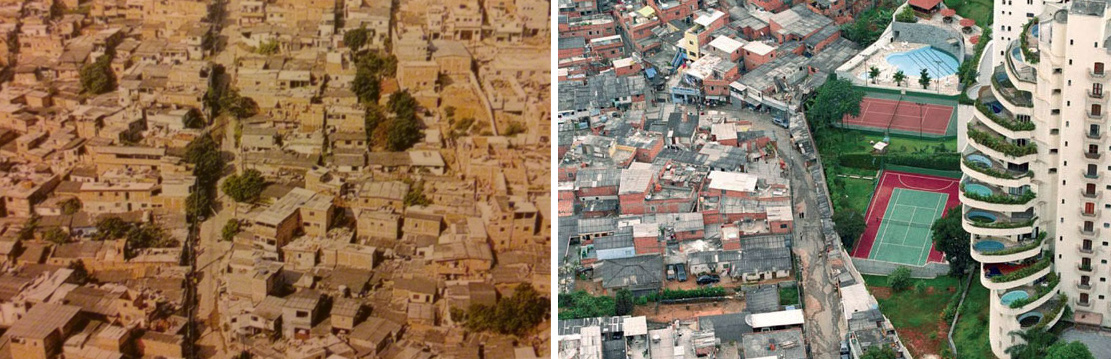
\includegraphics[width=1.0\textwidth]{./imagens/paraisopolis.jpg}%
    \end{center}%
    \fonte{Foto da esquerda de Gustavo Roth; foto da direita de Tuca Vieira/Folha Imagens, disponível em: \url{http://www.scielo.br/scielo.php?script=sci_arttext&pid=S0103-49792010000200005} Acesso em 11 de novembro de 2014}
\end{figure}%

Pode-se observar nos três pilares clássicos da sustentabilidade o papel relevante dos transportes. \citeauthoronline{VASCONCELLOS2012} (\citeyear{VASCONCELLOS2012}) aponta ainda que a energia gasta na mobilidade por habitante de uma cidade, ou seja, quanta energia os moradores de um município precisam para deslocar-se permite ter uma ideia do ``grau de sustentabilidade'' da mesmo. Dessa maneira, cabe uma breve discussão sobre transporte sustentável.

Para Black, um transporte sustentável seria aquele que atende às ``atuais necessidades de transporte e mobilidade não devem comprometer a capacidade das futuras gerações satisfazerem as suas próprias necessidades'' \cite[p.151]{BLACK1996}, e também que ``provê transporte e mobilidade com combustíveis renováveis, minimizando as emissões prejudiciais ao ambiente local e globalmente, e prevenindo fatalidades, lesões e congestionamentos desnecessários'' \cite[p.12]{BLACK2010}.

Banister (\citeyear{BANISTER2005,BANISTER2008}) aponta algumas medidas a serem perseguidas para que se possa alcançar um transporte sustentável:
\begin{compactitem}[]
\item (i) reduzir a necessidade de viajar;
\item (ii) encorajar a troca para modos de transporte coletivo ou não motorizado;
\item (iii) reduzir o comprimento das viagens;
\item (iv) incentivar a adoção de sistemas e tecnologias de transporte mais eficientes, tanto para carga quanto para passageiros;
\item (v) reduzir a utilização de carros e caminhões de carga nas áreas urbanas;
\item (vi) reduzir, na fonte, ruídos e emissões dos veículos,
\item (vii) incentivar a utilização mais eficiente e ambientalmente consciente do estoque de veículos;
\item (viii) melhorar a segurança de pedestres e de todos usuários das (rodo)vias;
\item (ix) melhorar a atratividade das cidades para seus moradores, trabalhadores, compradores e visitantes.
\end{compactitem}

Embora cientes (organismos internacionais, governos e comunidades científicas) de medidas que corroborariam para o estabelecimento de um transporte sustentável, os padrões de mobilidade observados indicam uma dependência cada vez maior do automóvel (com poucas exceções), seja nos países desenvolvidos \cite{BANISTER2005}, seja nos países em desenvolvimento \cite{VASCONCELLOS2012}. \citeauthoronline{BANISTER2005} (\citeyear{BANISTER2005}) informa que entre 1984 e 1994 houve um aumento de 31\% na posse de veículos e que estimava-se chegar a 50\% em 2020. Ele também indica que a maior aprte da forta (70\% em 2005) encontrava-se nos países desenvolvidos.

Entretanto, isso não significa que a posse de carros não esteja crescendo nos países em desenvolvimento. No Brasil, a frota de automóveis vem crscendo desde 1960 conforme pode ser observado na Tabela \ref{tab:venda-veic-br}, sendo que em 2009, 53\% da frota total de veículos era composta por automóveis \cite{VASCONCELLOS2012}. Esse fato somado ao de que o automóvel é o modo que apresenta o maior consumo energético (ver Tabela \ref{tab:gep-modo}) levam a concluir que os o desenvolvimento no Brasil também trilha o caminho da insustentabilidade.

\clearpage
\begin{table}[htb]
    \IBGEtab{%\renewcommand{\arraystretch}{1.5}%%\ABNTEXfontereduzida%
	    \renewcommand{\arraystretch}{1.5}
        \caption{Venda interna de veículos no Brasil entre 1960 e 2009}
		\label{tab:venda-veic-br}
    }{%
	    \begin{tabular}{p{2.00cm} P{4.0cm} P{4.0cm} P{4.0cm}}
            \toprule
	           \headerTabCenterCell{Ano} &
		       \headerCell{Autos} &
		       \headerCell{Total} &
		       \headerCell{Fator de crescimento (total)} \\
		    \midrule \midrule
		        1960&
		        40.980&
		        131.499&
		        1\\
		    \midrule
		        1970&
		        308.024&
		        416.704&
		        3,2\\
		    \midrule
		        1980&
		        739.028&
		        980.261&
		        7,5\\
		    \midrule
		        1990&
		        532.906&
		        712.741&
		        5,4\\
		    \midrule
		        2000&
		        1.176.774&
		        1.489.481&
		        11,3\\
		    \midrule
		        2009&
		        2.474.764&
		        3.141.240&
		        23,9\\
		    \bottomrule
		\end{tabular}
    }{%
		\fonte{Adaptado de \cite[p.29]{VASCONCELLOS2012}}
		}
\end{table}

\begin{table}[htb]
    \IBGEtab{%\renewcommand{\arraystretch}{1.5}%%\ABNTEXfontereduzida%
	    \renewcommand{\arraystretch}{1.5}
        \caption{Consumo energético teórico dos modos de transporte em lotação plena}
		\label{tab:gep-modo}
    }{%
	    \begin{tabular}{p{4.00cm} P{4.0cm}}
            \toprule
	           \headerTabCenterCell{Modo de Transporte} &
		       \headerCell{gramas equivalentes de petróleo para mover um passageiro por um quilômetro}\\
		    \midrule \midrule
		        ônibus comum&
		        4,1\\
		    \midrule
		        metrô&
		        4,3\\
		    \midrule
		        motocicleta&
		        11,0\\
		    \midrule
		        automóvel&
		        19,3\\
		    \bottomrule
		\end{tabular}
    }{%
		\fonte{Adaptado de \cite[p.84]{VASCONCELLOS2012}}
		}
\end{table}

Se parece ilógica e insustentável a adoção do automóvel particular como modo principal de locomoção, por que ele continua tão bem cotado? A resposta a essa pergunta parece ser uma soma de fatores que o leva a ser um ícone, culturalmente simbólico e economicamente valorizado. 
Sobre o caráter simbólico, \citeauthoronline{BANISTER2005} (\citeyear{BANISTER2005},. p.05) expõe que o carro é visto como ``seguro, sempre disponível e nunca muito longe do seu motorista''. \citeauthoronline{URRY2001} (\citeyear{URRY2001}) indica ainda outros fatores que contribuem para esse \emph{status} do carro: 
\begin{compactitem}[]
\item (i) como um objeto manufaturado, nascido com o fordismo, é um ícone do sucesso capitalista; 
\item (ii) depois da moradia, é o principal bem de consumo que confere \emph{status} social ao indivíduo;
\item (iii) é um objeto de suficiente complexidade que sintetiza e ilustra um avanço tecnológico;
\item (iv) confere mobilidade individual e, portanto, liberdade para algumas escolhas como horários de saída e rotas adotadas;
\item (v) é revestido de um discurso ela mídia e pela indústria cultural que o liga ao sucesso e ao progresso.
\end{compactitem}

Sob a perspectiva econômica, na indústria brasileira, o ramo automobilístico tem tido um papel bastante central. Nos anos 1950 foram instaladas as três maiores montadoras à época na região de São Bernardo (SP), o que gerou emprego, aqueceu a indústria e também estimulou o nascimento de toda uma geração de motoristas de carro. Desde então, há uma pressão crescente por por mais vias, maiores, melhores e mais fluidas.
%Em 1990, com a estabilização da economia e o controle da inflação, houve o fortalecimento do setor da construção civil e a popularização do financiamento de motos e carros. Esses elementos geraram uma megalópole com, por exemplo, \emph{shopping centers} que dispõem de gigantesca quantidade de vagas de estacionamento e condomínios com pelo menos uma vaga de garagem por apartamento, sem que tudo isso seja devidamente comportado pelos espaços de circulação.
Dado que o espaço é finito, ao aumentar os espaços de circulação, diminuem-se os espaços disponíveis para abrigarem as atividades das pessoas. Há mais de 50 anos \apudonline[p.63]{OWEN1956}{BLACK2010} já conseguia reconhecer que:

\begin{citacao}
O problema do congestionamento se tornou tão grande que muitas comunidades estão chegando à conclusão de nunca haverá avenidas nem vagas de estacionamento suficientes que permitam o movimento de todas pessoas em carros particulares.
\end{citacao}

A RMSP sofre das contradições de políticas que apontam para direções diferentes, quando não antagônicas. No âmbito do município de São Paulo, conta-se com a ``Lei de Mudanças Climáticas'' \cite{LEICLIMASP2009} que prevê a redução de 30\% nas emissões dos gases do efeito estufa, além de substituição integral do uso de combustíveis fósseis por renováveis na frota de transporte público. No âmbito estadual, o Plano de Controle de Poluição Veicular 2011-2013 \cite{PCPV2011} indica, entre outros objetivos, a adoção da inspeção ambiental de veículos, uma (única) medida que incide sobre o transporte privado individual. Já no âmbito federal, para garantir aquecimento econômico e minimizar a taxa de desemprego, o Imposto sobre Produtos Industrializados (IPI) dos carros nacionais novos 1.0 foi a zero no primeiro semestre de 2012, sendo que até o final de 2014 não terá retornado ao patarmar dos 11\% \cite{FAZENDA2014}.

Em alguma medida o conjunto das políticas públicas transparece um desejo de não restringir a posse do carro, mas seu uso. Ou seja, deseja-se ao mesmo tempo desviar do impacto econômico que uma diminuição das vendas de carros geraria e regular o uso dos automóveis. Essa é a abordagem liberal que diversas cidades, de vários países do mundo vem adotando. Isto é, não se deseja impor restrições legais ou econômicas, mas entender e estimular comportamentos mais interessantes para o conjunto da sociedade e que corrobore para a construção de cidades mais sustentáveis. Todavia, \apudonline[p.7]{GILBERT2000}{BANISTER2005} deixa o alerta de que ``há uma ligação entre a posse do carro e uso do carro, e qualquer estratégia coerente para reduzir o uso do carro está fadada ao fracasso se realmente não abordar a causa da mobilidade insustentável, ou seja, o carro''.

%Dessa maneira, recai-se na necessidade de articulação entre planejamento urbano, ambiental e econômico.


\clearpage
\section{Intersecções e Sobreposições}
% META: 10p.

Não apenas o movimento feminista e o embrião da concepção de gênero datam do final do século XIX; a intersecção entre gênero, mobilidade e sustentabilidade também. Em 1895, \citeauthoronline{WILLARD1895} publicou seu livro \emph{A Wheel whithin a Wheel} em que narra como ela, mulher, aos 53 anos, aprendeu a andar de bicicleta (ver Figura \ref{fig:willard}). Ela não escreveu um livro sobre mobilidade, nem sobre gênero, muito menos sobre sustentabilidade. Porém, ela aborda essas questões a partir dessa sua experiência. Ela toca na questão de gênero, por exemplo, ao falar do vestuário de uma ciclista:

\begin{citacao}
Se as mulheres pedalarem, ao fazê-lo elas devem vestir-se mais racionalmente do que foram acostumadas. E se elas fizerem isso, muitos preconceitos concernentes ao que elas estariam autorizadas a vestir cairão por terra. (Livre tradução de \citeauthoronline{WILLARD1895}, \citeyear{WILLARD1895}, p.39)
\end{citacao}

\begin{figure}[htb]%
    \caption{\label{fig:willard}Frances Willard aprendendo a andar de bicicleta}%
    \begin{center}%
        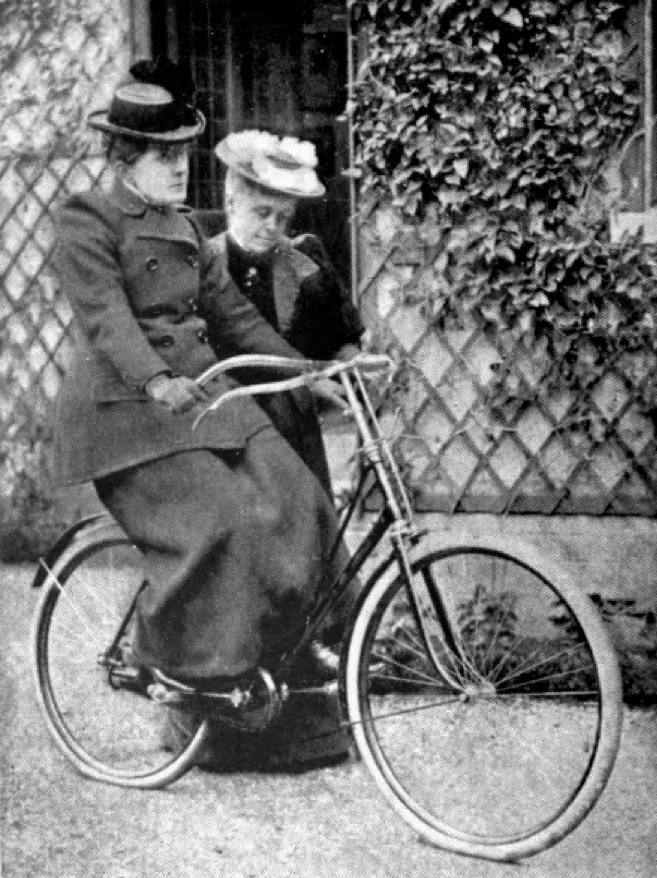
\includegraphics[width=0.37\textwidth]{./imagens/Willard-p56.jpg}%
    \end{center}%
    \fonte{\cite[p.56]{WILLARD1895}}
\end{figure}%

O que se esperava que uma mulher vestisse àquela época? Como pedalar com vestidos tão longos que sempre cobriam os pés e contavam com muitos babados, plissados, franjas e passamanarias
\footnote{Essas características da indumentária feminina utilizada no final do século XIX podem ser percebidas ora numa pintura de Cézanne (\emph{Madam Cézanne} num vestido vermelho, de 1888/1890), ora nas peças expostas no Museu da Moda em Canela (\url{http://www.museudamodadecanela.com.br/} - acesso em 15 de novembro de 2014) ou no \emph{The Metropolitan Museum of Art} (\url{http://www.metmuseum.org/toah/hd/wrth/hd_wrth.htm} - acesso em 15 de novembro de 2014).}?
%traje da Princesa Isabel: http://varelanoticias.com.br/vestido-usado-por-princesa-isabel-esta-em-exposicao/
%paperdolls vitorianas: https://casitadepapel.wordpress.com/2012/01/25/paper-dolls-victorianas/
Andar de bicicleta não foi para ela apenas um desafio por conta da habilidade manual requerida e/ou idade que possuía. Ao longo da obra ela retrata não apenas que ganhou mobilidade, ela adquiriu auto-confiança e vislumbrou possibilidades que antes não reconhecia, como aspirações relativas a seu crescimento pessoal. Ela constatou que a imobilidade física feminina atava-se a outras imobilidades, sociais. Assim, transformar a forma de se mover no espaço era (e é) também uma forma de transformar as relações de gênero \cite{HANSON2010}. E aqui o termo gênero é pertinente na análise da obra, e não anacrônico, porque tem no cerne as relações de poder estabelecidas entre indivíduos
\cite{SCOTT1986}, em função do que se entende por ``feminino'' e ``masculino''.
%Ao fim da obra ela revela as motivações que a levaram a isso, entre as quais estão o gosto pela aventura, o empoderamento e o fato de muitas pessoas terem-na dito que não conseguiria com sua idade. 
E embora a preocupação a respeito de sustentabilidade seja recente, extemporânea a \citeauthoronline{WILLARD1895}, vale notar que a liberdade adquirida por ela dá-se ao aprender a andar de bicicleta, um modo de transporte não motorizado, com emissões nulas de gases do efeito estufa, de manutenção pouco custosa e, cada vez mais, símbolo de sustentabilidade.

Os primeiros artigos que abordam explícita e articuladamente questões de gênero e de transporte datam do fim da década de 1970, como o editorial de \citeauthoronline{ROSENBLOOM1978} (\citeyear{ROSENBLOOM1978}), em que ela problematiza como serão distribuídas as atividades e, por conseguinte, as viagens da população frente ao fato de que a proporção de mulheres na força de trabalho vinha aumentando rapidamente
\footnote{Em 1978, 54\% das mulheres casadas dos Estados Unidos eram assalariadas, mais do que o dobro do que se constatou logo após o fim da Segunda Guerra Mundial \cite{ROSENBLOOM1978}.
\hl{dados do Brasil?}}. À época havia quem afirmasse que conforme as desigualdades salariais diminuíssem e os papeis sociais se alterassem, as diferenças nos padrões de viagens sumiriam. \citeauthoronline{ROSENBLOOM1978} discorda e, entre seus argumentos figura o de que as variáveis sócio-econômicas tradicionais pouco explicam com as relações de poder e os processos de decisão circunscritos ao ambiente doméstico. Outrossim, identifica-se que nas diversas classes socio-econômicas as mulheres que trabalham ainda continuam sendo as principais responsáveis pelas tarefas domésticas e pelo cuidado com as crianças. Um fato retratado pela autora ilustra o desconhecimento completo do fenômeno por parte dos órgãos oficiais de planejamento de transportes: cientistas contratados pelo \emph{U. S. Department of Transportation} chegaram a declarar que estimular os homens a usar o transporte público e  deixar o carro em casa poderia aumentar o consumo de energia e os níveis de poluição, pois as mulheres usariam o carro fazendo viagens mais curtas, em baixas velocidades e com maior consumo de combustível.

%\hl{>>> talvez para fechar o capítulo} Foi da década de 1980 pra cá que o assunto gênero e transporte passou a reter atenção, crescente, da comunidade científica. Pesquisadores(as) começaram a examinar os padrões de mobilidade com o recorte de gênero considerando que há entre os gêneros assimetria de poder, acesso desigual a recursos materiais e diferenças na escolha modal. São comuns duas abordagens, a primeira que considera principalmente as diferenças de gênero decorrentes do mercado de trabalho \cite{HANSON1985} e a segunda que prioriza as diferenças decorrentes do medo feminino da violência masculina \cite{TRENCH1992,GODDARD2006,LOUKAITOU2008}. O escopo deste trabalho se limita à primeira abordagem, o que não significa que a segunda abordagem seja menos importante - ambas são complementares.

Assim como foi para \citeauthoronline{WILLARD1895}, o ganho de mobilidade pode refletir melhores condições de vida para as mulheres. Não se pode esquecer que na maioria das vezes a viagem é atividade meio e não fim, ou seja, as pessoas precisam de um motivo para fazer uma viagem, querem chegar a algum lugar por um propósito. Caso uma mulher saísse de casa sem próposito, por exemplo no Brasil da década de 1970, seria questionada moralmente. Um homem também poderia ser considerado vagabundo na mesma situação - embora, há de se frisar, o julgamento moral sobre ele seria mais condescendente do que sobre ela. \citeauthoronline{DINCAO2012} (\citeyear{DINCAO2012}, p.\hl{XX}) relata que: 

\begin{citacao}
dos cronistas, viajantes e historiadores do período [\hl{XX}] nos exibem um quadro em que a menina ou a mulher [burguesa] candidata ao casamento é extremamente bem cuidada, é trancafiada nas casas, etc.
\end{citacao}


%>>>>> TRABALHO


Desta forma, uma das maneiras de adquirir liberdade de movimento foi poder ter motivos que não domésticos para sair de casa, o que não se deu - nem se dá - sem resistência, como o editorial de \citeauthoronline{ROSENBLOOM1978} já dava pistas. \apudonline{HANSON1995}{HANSON2010} constatara que as mulheres de Massachusetts, Estados Unidos, tinham dificuldade de encontrar \textbf{trabalho} no final dos anos 1980.
Mais recentemente, 
\citeauthoronline{ELMHIRST2003} (\citeyear{ELMHIRST2003}) apontam que mulheres sequer são consideradas para certos postos de trabalho na Indonésia porque não se supõem que possam estar fora de casa após escurecer. Em algumas vilas indianas, \citeauthoronline{RAJU2005} (\citeyear{RAJU2005}) ao caracterizar um projeto que visa o empoderamento feminino constata que uma das mudanças mais significativas detectadas foi o fato das mulheres poderem sair sozinhas de casa, isto é, poderem existir \emph{per si} no espaço público.
O ``ganhar a rua'' feminino é fundamentalmente ligado ao acesso ao trabalho, ao aumento da participação feminina na população economicamente ativa (\hl{Künzler, 1994}) e ao crescimento da renda individual.  \citeauthoronline{MANDEL2004} (\citeyear{MANDEL2004}) mostrou que mulheres que têm mais liberdade para fazer viagens têm maior renda em Porto Novo, Benin.
Mesmo ao considerar países com menor desigualdade
\footnote{Para medir a desigualdade é comum utilizar o Índice de Gini, cujos valores são tão mais altos quanto maior for a desigualdade da renda familiar. Estados Unidos apresentam um Índice Gini de 34 (2005); Indonésia, de 39,4 (2005); Benin, de 36,5 (2003); Noruega, de 25 (2008); e Brasil, de 55,3 (2001). Fonte: \url{https://www.cia.gov/library/publications/the-world-factbook/fields/2172.html} Acesso em 29 de novembro de 2014.}, como a Noruega, observar-se-á que as mulheres casadas trabalham em localidades mais próximas das residências e têm menos poder de escolha geográfico do que seus maridos no que tange às oportunidades de trabalho \cite{HJORTHOL2000}.

Não obstante, é preciso ter cuidado e não fazer uma relação identitária automática entre \textbf{mobilidade} e \textbf{empoderamento}.
Alterar padrões de mobilidade pode significar alterar relações de poder já que é de alguma forma requisito da acessibilidade à escola, ao trabalho, a hospitais, às lojas, às áreas de lazer, etc.
Então, maior mobilidade pode significar mais equidade em algumas situações, mas não necessariamente em todas. Isto é, não há uma relação biunívoca em que maior mobilidade leve, sempre, a mais acesso e oportunidades iguais a todas pessoas. Essas nuances podem ser observadas quando se perfaz uma abordagem interseccional, como fizeram \citeauthoronline{LAFFERTY1991} (\citeyear{LAFFERTY1991}), \citeauthoronline{LAFFERTY1992} (\citeyear{LAFFERTY1992}) e \citeauthoronline{CRANE2007} (\citeyear{CRANE2007}). \citeauthoronline{GILBERT1998} (\citeyear{GILBERT1998}) faz essa ponderação e encara como demasiado simplista entender a mobilidade como empoderamento e a imobilidade como sinal de falta de poder; afinal, é preciso considerar a espacialização dessa mobilidade, considerando suas características sociais, culturais e econômicas. Talvez uma pessoa se desloque menos por ter mais acesso a oportunidades num raio próximo do seu lar e este lar assim seja localizado porque essa pessoa desfruta de melhor posição social e econômica.


%>>>>> INTERSECCIONALIDADE


\citeauthoronline{LAFFERTY1991} (\citeyear{LAFFERTY1991}) indicam que maior mobilidade não significa mais poder, visto as condições sócioeconômicas de quem precisa fazer longas viagens para trabalhar em postos de baixa remuneração. Em artigo de \citeyear{LAFFERTY1992}, com base em dados referentes ao final dos anos 1980 do norte de Nova Jersei (Estados Unidos), \citeauthoronline{LAFFERTY1992} sustentam a hipótese que de as diferenças de gênero na segmentação do mercado de trabalho têm consequências sobre a distribuição espacial (desigual) das minorias. As autoras conseguem atingir uma \textbf{abordagem interseccional} entre raça, gênero e classe neste trabalho. As mulheres afro-descendentes, latinas e brancas distribuem-se de forma diversa no espaço urbano. As negras contam com tempos de viagem maiores e menor grau de confinamento espacial que as latinas e as brancas. A ``cidade da mulher negra'' é maior, mas nem por isso, melhor: elas têm menos acesso a oportunidades de trabalho em regiões próximas das suas residências e geralmente são empregadas em postos de baixa remuneração. A maioria desses postos, ligados ao setor de serviços e não ao de processos de manufatura, são menos vulneráveis ao desemprego. Os homens negros e latinos e as mulheres latinas são contratados mais freqeuntemente pelo setor manufatureiro e, portanto, são mais suscetíveis ao desemprego estrutural. Essa menor vulnerabilidade ao desemprego da mulher negra, contudo, não implica que as oportunidades de emprego lhes sejam mais acessíveis - elas precisam ir mais longe para consegui-las. Entre as mulheres, as latinas apresentam viagens relativamente curtas, próximo ao padrão das brancas. Porém, contam com alto grau de confinamento e a pior remuneração de todos os grupos analisados. Destarte, \citeauthoronline{LAFFERTY1992} mostram que analisar somente a classe (pela renda, poder de compra, posse de bens, grau de instrução associado), ou somente o gênero, ou somente a raça/etnia pode levar a conclusões muito triviais para fenômenos que são mais complexos. Em estudo mais recente, também nos Estados Unidos, que parte de bases de dados nacionais de 1985, 1995 e 2005, \citeauthoronline{CRANE2007} (\citeyear{CRANE2007}) observa que os tempos de viagens vêm convergindo quando consideradas as várias raças/etnias do mesmo gênero, em especial para mulheres. Ou seja, mulheres negras, brancas, asiáticas e latinas tendem a apresentar menos diferenças entre si ao longo do tempo. Analogamente, esse fenômeno também ocorre dentro do grupo masculino.


Embora a divisão de trabalho por gênero seja identificada como um fator que influencia a mobilidade, costuma-se ver o trabalho doméstico como uma restrição na participação do mercado de trabalho.
Subestima-se o efeito do arranjo familiar no padrão de atividades e de viagens geradas a partir de demandas domésticas.
Se no mercado de trabalho vem sendo traçado um caminho que tende a diminuir o desequilíbrio de gênero, no trabalho doméstico ainda é a mulher a grande responsável pela sua execução.
Cabe então, analisar as \textbf{viagens cujo motivo não seja o trabalho} e outros aspectos relacionados ao arranjo familiar: como a presença de criança interfere na rotina familiar e como se distribui o uso do automóvel entre os membros, quando este está presente.


%>>>> VIAGENS NÃO-TRABALHO


Em 1997, \citeauthoronline{ROOT1999} (\citeyear{ROOT1999}) indica que cerca de 50\% das viagens feitas por mulheres, nos Estados Unidos, por motivos pessoais (não trabalho) eram, na realidade, para a família.
\citeauthoronline{VANCE2007} (\citeyear{VANCE2007}) trabalham econometricamente com dados em painel da Alemanha, referente ao período de 1996 a 2003, indagando se o gênero desempenha papel relevante na determinação da probabilidade de utilização do automóvel ou da distância percorrida; e se assim o for, se seria esse papel influenciado por outros atributos socieconômicos do indivíduo ou de seu núcleo familiar. 
Os autores constataram que as mulheres realizam mais viagens do que os homens quando o motivo não é trabalho. E embora o volume de viagens delas seja maior, a relação de depenência do carro para este tipo de viagem é menor - elas utilizam mais outros modos.



%>>>>> PRESENÇA DE CRIANÇA NA FAMÍLIA

\citeauthoronline{VANCE2007} (\citeyear{VANCE2007} verificou que situação ocupacional (empregado(a) ou não), número de crianças na família (ver Figura \ref{fig:prob-uso-carro}), facilidade de acesso ao transporte público tiveram influência significativa nas viagens feitas por carro (que não para o trabalho), tanto para homens como para mulheres. Essas mesmas variáveis não influenciaram, porém, a distância média dirigida; apenas o acesso (ou não) ao automóvel incidiu sobre esse efeito. 

\begin{figure}[htb]%
    \caption{\label{fig:prob-uso-carro}Simulação de probabilidade de uso do carro em função do número de crianças na família, na Alemanha}%
    \begin{center}%
        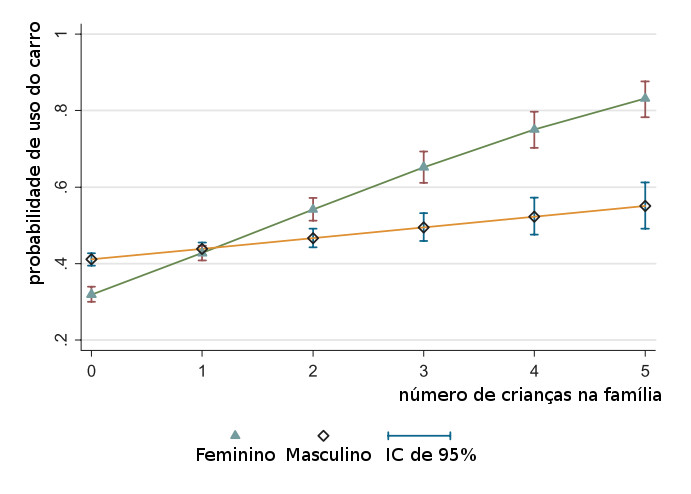
\includegraphics[width=0.8\textwidth]{./imagens/prob-uso-carro.jpg}%
    \end{center}%
    \fonte{Adaptado de \cite[p.59]{VANCE2007}}
\end{figure}%

A \textbf{presença de criança} é um fator que impacta bastante no padrão de atividades da família, de forma diferentes para pais e para mães. Ainda olhando para a Alemanha, estudo de \citeauthoronline{BEST2005} (\citeyear{BEST2005}) indica que mães usam menos frequentemente o carro do que mulheres sem filhos, ao passo que pais usam mais o carro do que homens sem filhos.
\citeauthoronline{GODDARD2006} (\citeyear{GODDARD2006}) identificaram que a presença de criança na família causa diferença significativa no comportamento de viagens entre homens e mulheres no norte da Califórnia (Estados Unidos). A presença de criança na família tem grande impacto na quantidade de tempo/distância que a mulher dirige automóvel, mas tal efeito não se observa no comportamento masculino. 
Esse comportamento pode se dever ao fato de que os homens, antes da paternidade, já estão mais familiarizados com o uso do carro e tendem a não trocar sua escolha modal. 
As mulheres, mães, tendem a ser mais pressionadas pelas atividades a serem cumpridas, que não o trabalho. Elas passam a absorver com mais facilidade a viagem de servir passageiro (a criança). Nesta conjuntura vale ressaltar que as escolas, em especial que atendem as crianças nas primeiras idades, geralmente ficam próximas à residência o que estimula que as viagens para levar crianças à escola sejam feitas a pé, pelas mães. Porém, as metodologias utilizadas nos grandes \emph{surveys}, tanto no Brasil como fora, pecam em detectar viagens curtas a pé. Nas Pesquisas OD da RMSP as viagens feitas integralmente a pé se estiverem num raio inferior a 500m da residência são desconsideradas.



%>>>>> POSSE E USO DO CARRO


\citeauthoronline{FOX1983} já apontava que em \citeyear{FOX1983} as mulheres nos Estados Unidos usavam menos o automóvel e mais o transporte público. Essa priorização masculina no \textbf{uso do automóvel} vem persistindo nos Estados Unidos \hl{REF} e também na Europa. \citeauthoronline{HJORTHOL2000} (\citeyear{HJORTHOL2000}) ao investigar mulheres e homens casados da região de Oslo, Noruega, observou que em famílias que dispunham de um carro, o marido detinha a prioridade do uso. \citeauthoronline{POLK2003} (\citeyear{POLK2003}) indica que os homens usam mais o carro, acumulam mais quilômetros percorridos por ano e fazem mais viagens como ocupantes únicos do que mulheres na Suécia.
Embora ter à disposição um carro para uso privado é o fator que mais influencia o seu uso em viagens motivo ``manutenção do lar'', segundo \citeauthoronline{BEST2005} (\citeyear{BEST2005}), na Alemanha, isso ainda não é suficiente para que as mulheres usem mais o carro do que os homens no geral. 
\citeauthoronline{BEST2005} (\citeyear{BEST2005}) elencam ainda outros fatores que estimulam o uso do carro: renda familiar e participação no mercado de trabalho. Assim, se há mais renda familiar, há mais condições financeiras de adquirir um carro para tê-lo à disposição. E se há mais pessoas na família que fazem parte do mercado de trabalho, há mais interesse em comprar um carro, seja por aumento da renda familiar, seja pela necessidade de modo com flexibilidade de rota.



%>>> SUSTENTABILIDADE


Portanto, as pesquisas apontam para o fato de que, \emph{ceteris paribus}, quando existe a posse do automóvel na família, este fica mais frequentemente à disposição dos homens do que das mulheres.
Dessa forma, as mulheres andam mais de transporte público e, ao andarem de automóvel: (i) são com maior frequência passageiras, remetendo à ideia de ``não andar desacompanhada fora de casa'', e (ii) servem passageiro mais frequentemente, remetendo às tarefas do cuidado \hl{ref hirata} com crianças e idosos \hl{ref rosenbloom?}.
Se isso por um lado reflete menor autonomia e independência das mulheres por construção histórica; por outro lado, percebe-se também que elas conscientemente indicam estar mais dispostas a uma migração modal para obter um padrão mais sustentável de deslocamentos do que eles. Mulheres e homens demonstram atitudes diferentes em relação à proteção do meio ambiente e à sustentabilidade, apesar da taxa de motorização feminina vir crescendo nos países mais industrializados \cite{ROOT1999}. \citeauthoronline{POLK2003} (\citeyear{POLK2003}) se propõe a estudar se, na Suécia, as mulheres são potencialmente mais adaptáveis a um sistema de transportes mais \textbf{sustentável} do que os homens. A autora conclui que sim, as mulheres tendem a expressar mais preocupação em relação as questões ambientais e declaram maior vontade de reduzir o uso do carro. 

Como foi possível depreender das seções anteriores deste capítulo, o carro é modo que mais ocupa espaço urbano e com maior consumo energético por pessoa, desta maneira, buscar um olhar de sustentabilidade sobre a análise de gênero e transportes é imprescindível. \citeauthoronline{SCHWANEN2002} (\citeyear{SCHWANEN2002}) indica que são variáveis importantes de análise do ponto de vista da sustentabilidade a \textbf{distância} viajada, o \textbf{modo} utilizado e o \textbf{tempo} de viagem - este último, embora às vezes não analisado, importa por ser um fator que pesa bastante nas decisões associadas à viagem (fazê-la ou não, que modo utilizar e que rota percorrer).


 
%>>DIST, MODO, TEMPO


\citeauthoronline{FOX1983} indicava os padrões de viagens das mulheres nos Estados Unidos em \citeyear{FOX1983}: elas faziam menos viagens, viagens mais curtas e rápidas. Quase dez anos depois, \citeauthoronline{IBIPO1992} (\citeyear{IBIPO1992}) revisita a hipótese de que mulheres fazem viagens mais curtas que homens em função de suas socialmente cosntruídas atribuições domésticas. O autor foca-se no tipo de família e toma para essa análise a variável número de trabalhadores(as) da família. Assim, constitui-se o grupo das famílias em que há um(a) trabalhador(a) e daquelas com dois trabalhadores(as). Com dados de Baltimore, Estados Unidos, no grupo em que o arranjo familiar conta com mais de uma pessoa que trabalha, as diferenças entre distâncias de viagens de homens e mulheres tendem a ser maiores - ainda que sejam controlados outros fatores como, por exemplo, presença de criança na família.
Nesse mesmo país, já no século XXI, \citeauthoronline{CRANE2007} (\citeyear{CRANE2007}) utiliza dados de 1985, 1995 e 2005 em suas análises e novamente afirma que mulheres fazem viagens mais curtas que homens. \citeauthoronline{CRANE2007} vai além e contesta estudos que apontam que o \emph{gender gap} dos tempos de viagem esteja diminuindo e das distâncias de viagem tenham até sumido em algumas áreas. Constata que ainda persistem diferenças: as distâncias percorridas por homens e por mulheres convergem muito lentamente e os tempos divergem.

Na Europa, o panorama se mantém semelhante com o dos Estados Unidos. \citeauthoronline{FAGNANI1983} (\citeyear{FAGNANI1983}) estuda os padrões de deslocamento das mulheres em Paris e constata que lá também elas desenvolvem viagens mais curtas.
\citeauthoronline{SCHWANEN2002} (\citeyear{SCHWANEN2002}), a partir do \emph{National Travel Survey} holandês de 1998, analisam tempo, motivo e modo da viagem. Encontram evidências que fatores sóciodemográficos (gênero, número de trabalhadores(as) na família, idade e grau de instrução) e contexto espacial da localização da residência influenciam o tempo médio de viagem diário. Os efeitos da posse de carro e da renda se dão de forma indireta, pois refletirão na escolha modal ou no número de trabalhadores(as) da família, segundo os autores. Do ponto de vista da interação com características urbanas, os tempos de viagem de carro tendem a aumentar quanto maior for o grau de urbanização e quanto mais policêntrica for uma região.

No conjunto Àsia e Oceania, o diagnóstico permanece.
Ao analisar as viagens motivo trabalho da região metropolitana de Melbourne, Austrália, \citeauthoronline{HOWE1982} (\citeyear{HOWE1982}) expõe que as taxas de participação feminina na força de trabalho australiana são baixas, levanta a hipótese de que isso se dê por alguma dificuldade de acesso às oportunidades de trabalho. Constata que mulheres fazem viagens mais curtas que homens e conlcui que para incrementar a participação feminina no mercado de trabalho é preciso também melhorar a distribuição espacial de ofertas de emprego.
\citeauthoronline{SONG2003} (\citeyear{SONG2003}) também constata que para Seul, Coreia, tanto os tempos quanto as as distâncias de viagens são menores paras as trabalhadoras. Nessa cidade, trabalhadores(as) solteiros(as) contam com distâncias de viagem maiores que os(as) casados(as) e, merece destaque o detalhe de que trabalhadores cujas esposas trabalham têm viagens mais curtas do que aqueles cujas esposas não trabalham. Por fim, \citeauthoronline{SONG2003} aponta que a responsabilidade por cuidar das crianças é um fator de encurtamento das viagens das mulheres casadas coreanas.

Na América Latina ... \hl{ainda não achei estudos sobre AL :-( }



% >>CADEIA DE VIAGENS


\citeauthoronline{MCGUCKIN1995} (\citeyear{MCGUCKIN1995}), com base no  \emph{Nationwide Personal Transportation Survey} de 1995 estadunidense examinam o \textbf{encadeamento de viagens} feitas durante a semana de homens e mulheres em fase adulta. Cosntatam que mulheres fazem cadeias de viagens com mais segmentos para que possam acomodar suas responsabilidades domésticas. Essa segmentação é ainda mais sentida por elas quando se conta com a presença de criança na família. As autoras ainda apontam que uma mudança na dinâmica doméstica em relação às tarefas e responsabilidades.
Dez anos depois, \citeauthoronline{MCNUCKIN2005} (\citeyear{MCNUCKIN2005}) publicaram estudo sobre o encadeamento de viagens com início na residência e término no trabalho de acordo com gênero e ciclo de vida a partir de base de dados nacionais dos Estados Unidos de 2001. Constataram que em lares com pai e mãe, em que ambos trabalham, as viagens cujo propósito de servir passageiro é deixar as crianças na escola têm maior probabilidade de serem acomodadas na cadeia de viagens da mulher do que do homem.
Na Europa, situação semelhante é encontrada. Na Espanha e no Reino Unido, em 1997, grande parte das viagens femininas era para servir passageiro, em sua maioria, filhos(as) \cite{ROOT1999}. 
Em Oslo, mulheres casadas fazem mais encadeamento de viagens por conta de responsabilidades domésticas do que homens casados \cite{HJORTHOL2000}.
Logo, se houve algum rearranjo na divisão de tarefas domésticas, essa mudança não foi profunda o suficiente para gerar alterações perceptíveis nos padrões de deslocamentos de homens e mulheres em diversos países.


%>>>GÊNERO E MOBIliDADE & VICE-VESA

Como o gênero configura e influencia a mobilidade, e como a mobilidade configura e influencia o gênero é o foco da discussão empreendida por \citeauthoronline{HANSON2010} (\citeyear{HANSON2010}). Entretanto, o mais comum na pesquisa quando ocorre a abordagem de gênero e mobilidade é um campo de conhecimento olhar o outro, com pouco esforço de buscar literatura ou metodologia de intersecção entre as áreas e, com isso, parte-se de conceitos e hipóteses que conduzem a resultados pouco convergentes ao final. \citeauthoronline{HANSON2010} (\citeyear{HANSON2010}, p.09) afirma ainda que em geral o debate ocorre em termos muito genéricos em torno da mobilidade/imobilidade com reflexos de uma ideologia dual que identificam a mulher/feminilidade com a casa, o espaço doméstico, movimentos restritos e o homem/masculinidade com a rua, o espaço público, movimentos livres. Enxergar o mundo a partir de um código binário de gênero foi uma construção longa e aboli-la por completo é uma tarefa a que este trabalho não se propõe, embora sempre que possível tente considerar a categoria como não binária.

A maior parte da literatura revisada diz respeito aos países do hemisfério Norte, mais industrializados, concentrando-se na Europa e nos Estados Unidos. Isso deve-se principalmente a dois fatores: (i) são países em que os temas gênero, transporte e sustenatbilidade são mais sistematicamente investigados; (ii) alguns países da Ásia também têm alguma produção dentro da temática desta pesquisa, mas muitas vezes em língua que não é de grande difusão no ocidente (como mandarim ou coreano). O que realmente chama a atenção é a parca literatura a respeito da América Latina. A maioria dos estudos encontrados baseiam-se em grandes bases de dados quantitaivos que são tratados de forma agregada. Daí, conclui-se que os comportamentos agregados de homens e  mulheres são diferentes, em diversos países e continentes. Uma série de aspectos relacionados à viagem são analisados para fazer essa constatação: quantidade por pessoa, tempo, distância, encadeamento, modo e motivo. Outros aspectos, ligados às caracaterísticas de indivíduos, são frequentemente envolvidos nas análises: gênero, idade (estágio do ciclo de vida), estado civil, presença de filhos na família, papel exercido dentro da família, situação ocupacional e renda.


%As grandes compras geralmente são feitas utilizando-se o carro, especialmente num contexto de padrão de consumo em que se expandem os grandes hipermercados, no Brasil, que precisam de grandes áreas urbanas e vendem em grandes volumes. Desta forma, estes empreendimentos têm localização menos central e buscam estar próximos de grandes avenidas. Essas condições de contorno (facilidade de acesso por carro e estímulo a grande volume de compras) tendem a levar o usuário a preferir o carro como meio de transporte.

%Já as pequenas compras geralmente são feitas a pé e estas são majoritariamente feitas pelas mulheres. Trata-se da compra diária na padaria, na farmácia, no mercado do bairro, entre outras. Porém, no Brasil, as pesquisas Origem-Destino costumam ignorar as viagens feitas a pé num raio inferior a 500m, o que inclui grande parte das viagens de “manutenção” como as de pequenas compras de abastecimento doméstico (Metrô, 2007).


%No Brasil, o olhar integrador entre transportes, planejamento urbano, meio ambiente e aspectos sociais tem sido cada vez mais frequente. Dois exemplos são o Estatuto da Cidade (\citeyear{ESTATUTOCIDADE}), obrigatório para cidade com mais de 20 mil habitantes, e o Plano Nacional de Mobilidade Urbana (\citeyear{PNMU}), obrigatório para cidades com mais de 500 mil habitantes. Tratam-se de dois instrumentos legais que norteiam elaboração de políticas públicas e, de acordo com \citeauthoronline{IEMA2010}(\citeyear{IEMA2010}):

%\begin{citacao}
%Estatuto da Cidade estabelece o direito às cidades sustentáveis para a atual e as futuras gerações, [sendo esse direito] compreendido como o acesso ao solo urbano, moradia, saneamento, infraestrturua, trabalho, lazer e serviços públicos.
%\end{citacao}

%\begin{citacao}
%A descrição e análise dos fenômenos de megalopolização que ocorrem durante os últimos 500 anos surpreendem pela convergência de padrões na maioria das megalópoles latino-americanas aqui apresentadas. Eles não podem ser atribuídos à história, mas apontam para forças macroestruturais que promovem um desenvolvimento urbano que converge para a ``insustentabilidade'' das megalópoles na era da globalização. \cite{FREITAG2007}
%\end{citacao}

%All else being equal, the average commuting time and the modal split in European cities are more strongly associated with the distribution of employment and population across the urban area and with urban siz \cite{SCHWANEN2002a}
% ----------------------------------------------------------
% Capitulo de Métodos
% ---
% ---
% Capitulo Métodos
% ---
\chapter{Métodos}\label{chap:metodo}
% META: 10p.

YYYYYYYYYYY

constructo como sendo uma definição mental de uma ideia de pesquisa, estabelecida com base na teoria subjacente e/ou na experiência e na intuição do pesquisador

Entre os vários modos de transporte, o automóvel é a forma geralmente de maior atratividade. Mas, apesar de seus apelos, um grupo particular de pessoas chama a atenção em relação ao uso diferenciado que fazem do automóvel: as mulheres. Historicamente, estas usam menos o automóvel em relação aos homens. Esta pesquisa de mestrado busca identificar e entender as estratégias utilizadas pelas mulheres em seu acesso em geral mais restrito ao automóvel particular e como este fato afeta seus padrões de atividades e viagens, com o objetivo de formular políticas públicas que estimulem comportamentos similares, menos dependentes  do uso do automóvel.


Strictly the term “sustainable transportation” has little academic meaning
following the World Commission on Environment and Development Commission’s
(Brundtland) Report that initially defined the parameters of sustainable
development and that highlights as its main theme the interconnectivity of
all forms of activity. Here we use the term “sustainable transportation” in
the more popular, journalist sense of reducing the environmental impacts of
transportation.
% ----------------------------------------------------------
% Capitulo de Análises Realizadas
% ---
% ---
% Capitulo Análises Realizadas
% ---
\chapter{Análises Preliminares}\label{chap:analises-preliminares}
% META: 15p.

\section{Periodicidade e Objetivos da Pesquisa Origem Destino}\label{sec:period-obj}

A Pesquisa Origem Destino (Pesquisa OD) é realizada a cada dez anos pela Companhia do Metropolitano de São Paulo (Metrô-SP), a partir de 1967. Assim, até hoje foram realizadas cinco Pesquisas OD realizadas (1967, 1977, 1987, 1997 e 2007), das quais este trabalho abrangerá as quatro últimas, cobrindo uma janela temporal de 30 anos. O intervalo de dez anos foi considerado pelo Metrô-SP muito longo mediante as rápidas transformações no espaço urbano; assim, em 2002 e em 2012 foram feitas Pesquisas de Aferição, com menor amostragem e zonas mais agregadas. Cabe esclarecer que estas pesquisas de aferição não serão objeto de análise do presente estudo.

A Pesquisa OD nasceu com a missão de compor uma base de dados que servisse de suporte a decisões de planejamento de transporte urbano na Região Metropolitana de São Paulo, que hoje abarca 38 municípios, além de São Paulo. Hoje, além de cumprir esse papel, também é ferramenta de suporte para o planejamento urbano de maneira mais sistêmica, bem como para a formulação de políticas públicas segmentadas, nas áreas de educação, saúde e segurança pública, por exemplo \cite{MANUALOD2007}.

\section{Descrição da Pesquisa OD}\label{sec:descricao-OD}

A Pesquisa OD é composta de duas partes complementares, a saber, a Pesquisa Domiciliar e a Pesquisa de Linha de Contorno. A Pesquisa Domiciliar tem como escopo as viagens internas à Região Metropolitana de São Paulo (RMSP), nela são escolhidos domicílios por amostragem, cujo critério será melhor discutido adiante, em que todos habitantes respondem a um questionário estruturado referente às viagens feitas no dia útil anterior à pesquisa. Já a Pesquisa de Linha de Contorno monitora pontos de entrada e saída (limites) da RMSP a fim de captar as viagens com origem dentro da RMSP e destino fora, vice-versa, ou ainda viagens que a atravessam. O presente trabalho tem como foco as viagens feitas internamente à RMSP, portanto, as bases de dados consideradas serão apenas aquelas advindas das Pesquisas Domiciliares.

A Pesquisa OD considera a dimensão espacial dos deslocamentos considerando as zonas de origem e de destino. Tais zonas tiveram seus limites alterados e área total expandida desde 1967. Na Tabela \ref{tab:carac-dados} é possível observar quantos municípios da RMSP foram envolvidos em cada pesquisa e em quantas zonas eram divididos. A coorespondência entre as diversas zonas é feita por uma unidade de compatibilização chamada Unidade de Correspondência de Zona (UCOD), em relação às quais todas zonas têm referência. Para que seja possível realizar uma análise de evolução temporal conjugando dados de diversas OD é preciso organizar todas informações de maneira coerente, assim, é apresentado no Anexo \ref{chap:anexo_ucod} as 67 UCOD  com as respectivas zonas correspondentes para 1977, 1987, 1977 e 2007. Para tal consolidação ser feita, parte das informações foi recebida do Metrõ-SP e parte foi fruto de compilação própria.


\begin{table}[htb]
    \IBGEtab{%\renewcommand{\arraystretch}{1.5}%%\ABNTEXfontereduzida%
	    \renewcommand{\arraystretch}{1.5}
        \caption{Caracaterísticas Amostrais das Pesquisas OD}
		\label{tab:carac-dados}
    }{%
	    \begin{tabular}{P{2.00cm} P{4.0cm} P{4.0cm}}
            \toprule
	           \headerTabCenterCell{Ano} &
   	           \headerTabCenterCell{Zona} &
		       \headerCell{Municípios da RMSP}\\
		    \midrule \midrule
				1967&
				15&
		        206\\
		    \midrule
		        1977&
		        27&
		        243\\
		    \midrule
		        1987&
		        39&
		        254\\
		    \midrule
		        1997&
		        39&
		        389\\    
		    \midrule
		        2007&
		        39&
		        460\\    
			\bottomrule	
		\end{tabular}
    }{%
		\fonte{Compilação a partir de {\cite{OD77,OD87,OD97,OD07}}}
		}
\end{table}


\subsection{Dados Coletados}\label{subsec:dados-coletados}

A Pequisa OD coleta dados referentes a viagens, indivíduos, famílias e domicílios, o que possibilita buscar relações entre características de deslocamentos e de indivíduos (e respectivas famílias e domicílios), e também características socioeconômicas. A amostra de domicílios é do tipo estratificada por faixas de consumo de energia elétrica - isso se dá por dois fatores: (i) as concessionárias possuem uma bases cadastrais de registro de domicílios mais confiáveis e representativas; (ii) ``o consumo de energia elétrica tem correlação com a renda familiar, que por sua vez tem correlação com o número de viagens da família'' \cite[p.10]{MANUALOD2007}. Esse esquema de amostragem estratificada buscou, em todos anos obter npível de confiança de 95\%. Nas zonas em que não foi possível utilizar esse arranjo, foi feita amostra causal simples, com erros em tornode 7,5\%. Na Tabela \ref{tab:tam-amostra} é possível observar algum dados relativos às amostras.
%TODO confirmar esse 7.5% com Emilia, bem como de o IC foi 95% sempre

Definido o tamanho da amostra total, define-se o tamanho de amostra para cada zona e a partir daí, procede-se um sorteio de endereços por fiaxa de consumo energético - etapa esta realizada pelas concessionárias, que fornecem ao Metrô-SP apenas os endereços dos domicílios selecionados, além de alguns adicionais para substituição caso necessário. Os selecionados recebem comunicação oficial por carta do Metrô-SP contendo as informações pertinentes à pesquisa. Quando no domicílio, os(as) pesquisadores(as) aplicam o questionário a todas pessoas que moram ali.


\begin{table}[htb]
    \IBGEtab{%\renewcommand{\arraystretch}{1.5}%%\ABNTEXfontereduzida%
	    \renewcommand{\arraystretch}{1.5}
        \caption{Caracaterísticas Gerais das Pesquisas OD}
		\label{tab:tam-amostra}
    }{%
	    \begin{tabular}{P{2.00cm} P{4.0cm} P{4.0cm} P{4.0cm}}
            \toprule
	           \headerTabCenterCell{Ano} &
   	           \headerTabCenterCell{Domicílios} &
		       \headerCell{Pessoas entrevistadas do sexo feminino} &
   		       \headerCell{Pessoas entrevistadas do sexo masculino}\\
		    \midrule \midrule
				1967&
				Não disponível&
				Não disponível&
		        Não disponível\\
		    \midrule
				1977&
				26.132&
				55.868&
		        52.161\\
		    \midrule
				1987&
				26.070&
				57.637&
		        53.176\\
		    \midrule
				1997&
				23.841&
				51.454&
		        57.326\\
		    \midrule
		        2007&
		        29.957&
		        53.561&
		        51.732\\    
			\bottomrule	
		\end{tabular}
    }{%
		\fonte{Compilação a partir de \cite{OD77,OD87,OD97,OD07}}
		}
\end{table}

A coleta, consistência e digitação do dados são de responsabilidade de institutos de pesquisa contratados pelo Metrô-SP e que variaram ao longo do tempo. Após a consolidação primeira do banco de dados, são aplicados fatores de expansão aos resultados amostrais. Primeiro aplica-se aos domicílios, às famílias e às pessoas pesquisadas segundo as expressões \eqref{eq:fator-expansao-dom}, \eqref{eq:fator-expansao-fam} e \eqref{eq:fator-expansao-pess}. Depois determina-se o fator de expansão das viagens. As viagens de quem usaou o modo metrô são expandidas levando em consideração a entrada de passageiros no sistema Metrô-SP na data de referência da pesquisa. Situação análoga ocorre com o trem metropolitano. As viagens de quem usou outro modo que não metrô e/ou trem teve seu fator de expansão de viagens determinado pelo total de passageiros transportados pelo sistema de ônibus (em 2007 foram utilizados os dados provenientes de Bilhete Único da SPTrans).

\begin{equation}\label{eq:fator-expansao-dom}
\mbox{Fator de expansão de domicílio}_i = \frac{\mbox{Total de domicílios da zona}_i}{\mbox{domicílios da amostra da zona}_i}
\end{equation}

%Referênciando a equação \ref{eq:fator-expansao} ou usando \eqref{eq:fator-expansao}.

\begin{equation}\label{eq:fator-expansao-fam}
\mbox{Fator de expansão da família}_i = \frac{\mbox{Total de famílias da zona}_i}{\mbox{famílias da amostra da zona}_i}
\end{equation}

\begin{equation}\label{eq:fator-expansao-pess}
\mbox{Fator de expansão da pessoa}_i = \frac{\mbox{Total de pessoas da zona}_i}{\mbox{pessoas da amostra da zona}_i}
\end{equation}

Vale fazer algumas considerações acerca da renda familiar. Nem todas pessoas respondem qual é a renda familiar, e como trata-se de uma das informações mais importantes para descrever o comportamento das pessoas \hl{FALTA REF} nestes casos, a renda é atribuída, mas não sem critério. A atribuição da renda familiar tem origem em expressão de regressão linear feita a partir de pontuação estabelecida por algum critério nacional
\footnote{Em 2007 foi usado o Critério Brasil, criado em 1996 pela Associação Nacional de Empresas de Pesquisa, e adotado por seus associados como padrão de segmentação da população em categorias de capacidade de consumo. Fonte: \url{http://www.abep.org/new/criterioBrasil.aspx}}, que variou ao longo do tempo - tais informações podem ser vistas no Quadro \ref{qua:atrib-renda}. 
A função dessas regressões é estimar o poder de compra das pessoas, agrupando-as em classes econômicas, a partir da posse de bens de consumo e do grau de instrução ''do chefe da família''. Nesses critérios de classificação econômica existe a orientação de que a categoria automóvel não deve considerar táxis, vans, \emph{pickups} usadas para fretes ou qualquer veículo usada para atividades profissionais, nem tampouco devem ser considerados veículos de uso misto (lazer e profissional) \cite{CRITERIOBRASIL}. Essa mesma orientação em relação aos automóveis é feita pelos manuais das Pesquisas OD \cite{OD77, OD87, OD97, OD07} tornando o conjunto coerente.
Nas famílias em que não se obteve nem declaração da renda, nem informações suficientes sobre bens de consumo, a renda foi atribuída à família a partir da mediana da zona a que pertencia e com mesmo grau de instrução da ``chefe da família''.

\begin{quadro}[htb]
    \IBGEtab{
        \renewcommand{\arraystretch}{1.5}
        \ABNTEXfontereduzida
        \caption[Dados para atribuição de renda familiar]{\label{qua:atrib-renda}Dados para atribuição de renda familiar}
	}{%
        \begin{tabular}{|P{2.0cm}|P{2.00cm}|P{5.00cm}|P{3.50cm}|}
           \hline
		       \headerCenterCell{Ano} & 
		       \headerCenterCell{Mês de Referência} & 
		       \headerCenterCell{Critério de Classificação} & 
		       \headerCenterCell{Índice de Correção*}\\ 
		    \hline\hline
		        1977&
		    	\hl{aguardando resposta Emilia}&
		        Função do Salário Mínimo&
		        \hl{??}\\
		    \hline
		    	1987&
		        setembro&
		        Critério ABA/ABIPMEPE (análogo ao Critério Brasil)&
		        0,000010223607163\\
		    \hline
		    	1997&
		        outubro&
		        Critério Brasil (ABIPMEPE)&
		        1.419,28\\
		    \hline
		    	2007&
		        outubro&
		        Critério Brasil (ABEP)&
		        2.755,34\\
			\hline
		\end{tabular}
	}{%
		\fonte{Compilação de informações obtidas por meio de correspondência eletrônica com Metrô-SP}
		\nota{Não existem informações de INPC anteriores a 1980. Portanto, foi utilizado o IGP do Ministério do Trabalho de acordo com metodologia indicada por {\citeauthoronline{IPEA2002} (\citeyear{IPEA2002})}}
    }
\end{quadro}


\subsection{Conceitos Adotados}\label{subsec:conceitos}

A seguir, são replicados alguns conceitos utilizados pelo Metrô-SP no desenvolvimento das Pesquisas OD, a saber, \emph{família}, \emph{modo coletivo}, \emph{modo individual}, \emph{modo não motorizado}, \emph{modo motorizado}, \emph{modo principal}, \emph{respondente qualificado}, \emph{viagem}, \emph{viagem a pé}, \emph{zona}: 

\begin{compactitem}[]
\item (i) É considerada \emph{família}: uma pessoa que more só; ou um conjunto de pessoas ligadas por laços de parentesco ou de dependência econômica que morem no mesmo domicílio; ou conjunto de, no máximo, cinco pessoas que mesmo não tendo laço de parentesco morem num mesmo domicílio. O(a) empregado(a) doméstico(a) que more com algum outro parente na casa do patrão será considerada como outra família, mas caso o(a) empregado(a) more sozinho(a) na residência onde trabalha, será considerado(a) como parte da família do empregador.

\item (ii) É considerado \emph{modo coletivo} o metrô, o trem, o ônibus, o microônibus, o transporte fretado, o transporte escolar, a lotação, a van, o trólebus.

\item (iii) É considerado \emph{modo individual} o automóvel, o táxi, a motocicleta e a bicicleta.

\item (iv) São considerados \emph{modos não motorizados} os modos a pé e de bicicleta.

\item (v) São considerados \emph{modos motorizados} os demais modos exceto a pé e de bicicleta.

\item (vi) \emph{Modo principal} é o modo de maior hierarquia dentre os modos utilizados numa mesma viagem. A hierarquia desses modos é a seguinte, nesta ordem, do que predomina sobre qual: metrô, trem, ônibus, transporte fretado, transporte escolar, lotação, táxi, dirigindo automóvel, passageiro de automóvel, motocicleta, bicicleta, outros e a pé.

\item (vii) \emph{Respondente qualificado} é a pessoa com 10 anos ou mais, residente no domicílio sorteado e capaz de responder às perguntas feitas pelo pesquisador. Uma pessoa responsável pode fornecer informações referentes às pessoas menores de 10 anos ou crianças maiores de 10 anos, pessoas doentes, ou que não fossem capazes de responder ao questionário.

\item (viii) \emph{Viagem} é uma atividade secundária e refere-se ao deslocamento de uma pessoa, por motivo específico, entre dois pontos determinados (origem e destino), utilizando, para isso, um ou mais modos de transporte. Sendo nominado como origem o local onde a pessoa entrevistada se encontrava quando iniciou o seu deslocamento, e como destino o local para onde a pessoa entrevistada se dirigiu (destino final).

\item (ix) \emph{Viagem a pé} é aquela realizada integralmente a pé, da origem ao destino. Além disso, só será contabilizada como viagem a pé se a distância percorrida é superior a 500m (ou cinco quadras) ou se o motivo da viagem é trabalho ou escola, independente da distância percorrida.

\item (x) \emph{Zona} de pesquisa é a unidade territorial de levantamento da origem e do destino das viagens, sendo a menor unidade para a qual está garantida a validade estatística das informações.
\end{compactitem}

%Índice de mobilidade: relação entre o número de viagens e o número de habitantes de uma determinada área
%Taxa de motorização: número de automóveis por mil habitantes.

Como este estudo baseia-se em dados secundários é preciso estar ciente das limitações que conceitos e metodologia de pesquisa adotados podem trazer. O conceito de família é bastante centrado na unidade do domicílio o que pode desconsiderar laços afetivos e redes de solidariedade que as famílias ensejam, mesmo estando em domicílios separados. Por exemplo, uma criança pequena cujos pais precisam trabalhar, pode significar que vá haver viagens motivo escola, com um dos pais, mais provavelmente a mulher, servindo passageiro. Entretanto, a depender da oferta de serviços do local de residência, pode ser que não haja vaga em creche disponível. Pode ser ainda que a família não disponha de  condições financeiras para pagar uma escola particular para esa criança. Um arrranjo muitas vezes adotado é deixar a criança com avós ou tios que morem próximos. Isso representa impacto no padrõa de mobilidade e também uma ``economia'' que o arranjo familiar proporciona. Esses arranjos e nunaces pouco serão percebidos a partir destas bases de dados pela forma com que foram construídas.

Outra limitação que merece atenção, é a hierarquia estabelecida entre os modos. Muito embora haja a descrição dos modos utilizados (até três em 1977 e 1987 e até quatro em 1997 e 2007), a duracao da viagem disponível no banco de dados é a duração total, geralmente atribuída ao modo principal. Contudo, as viagens por modos não morotizados são as menos ``fortes'' na hierarquia de modos, sendo consideradas praticamente se forem exclusivas. Isso dificulta e às vezes impossibilita analisar devidamente os modos não morotizados dentro das cadeias de viagens. 
Ademais, existe uma subrepresentatividade das viagens a pé devido ao conceito adotado. E espera-se que estas viagens sejam importantes na descrição diferencial dos padrões de deslocamente de acordo com os gêneros.  A a mulher muitas vezes é responsável pelas tarefas ligadas à administração doméstica \hl{REF}, o que inclui compras rápidas e próximas à residências \hl{REF}, muitas vezes feitas a pé \hl{REF} - como ir à padaria, à farmácia, acompanhar filhos até o ponto de ônibus, por exemplo.


\section{Bancos de Dados}\label{sec:bd}

Afim de tornar possível comparar dados das diversas Pesquisas OD de análise foi necessário conhecer o banco de dados de cada edição, e para que seja possível estabelecer alguma análise sobre evolução de padrões de mobilidade e comportamento, é preciso que os dados dos diversos bancos sejam comparáveis. Para isso, foi desenvolvido o desenho de um novo banco de dados, com função de integrar e compatibilizar as informações julgadas relevnates até este momento, e também aquelas que suspeita-se que possam vir a ser relevantes em etapas posteriores do trabalho. Os \emph{layouts} dos bancos de dados originais podem ser observados no Anexo \ref{chap:anexo_layouts}, e o do  banco integrador pode ser visto no Quadro \ref{qua:layout-haydee}.

Alguns procedimentos realizados na integração dos bancos de dados não foram óbvios e merecem comentários:
\begin{compactitem}[]
\item(i) No campo TIPO_DOM em 1977 e 1987 existiam somente as categorias particular e coletivo; já em 1997 e 2007 passou a existir também a categoria favela. Foram adotadas as categorias das OD-1997 e OD-2007, o que indica que para os anos de 1977 e 1987 a categoria favela (3) ficará vazio (artificialmente).
\item(ii) No campo COND_MORA a categoria adotada ``outros'' abarca as categorias originais ``cedida'', ``outros'' e ``não se aplica''.
\item(iii) Não foram mantidos os bens de consumo, pois a função deles é servir de \emph{input} para determinar a renda atribuída da qual já se dispõe. Apenas os bens que são meios de transporte foram mantidos (automóveis, motocicletas e bicicletas).
\item (iv) No campo ESTUDA foram adotadas as categorias sim (1) e não (2). Em 1987, 1997 e 2007 há a categoria ``não'', cuja correspondência é direta. As demais tornaram-se ``sim'', independente das subdivisões que apresentam. Em 1977, porém, essa variável não existe. Neste caso, se o campo de zona da escola fosse não vazio, portanto, a pessoa era considerada estudante.
\item (v) No campo OCUPACAO as classificacoes de cada ano são bastante diferentes. Assim, decidiu-se por discriminar quem não respondeu, quem é estudante, quem é dono(a) de casa, que é aposentado(a), quem não tem ocupação (como por exemplo, crianças), quem está desempregado(a), quem está em licença e quem trabalha (em todas opções possíveis dadas em todas as Pesquisas OD).
\item(vi) No campo SETOR_ATIV nos anos em que há opção de indicar o setor de mais de um trabalho (caso a pessoa tenha mais de um trabalho), foi considerado o setor do primeiro trabalho.
\item(vii) Os campos de coordenadas CO_DOM_X, CO_DOM_Y, CO_ESC_X, CO_ESC_Y, CO_TRAB1_X, CO_TRAB1_Y, CO_TRAB2_X, CO_TRAB2_Y, CO_ORIG_X, CO_ORIG_Y, CO_DEST_X, CO_DEST_Y foram preenchidos com informações de coordenadas no ano de 2007, pois esses dados eram disponíveis. Para os demais anos serão adotados os centroidesdas subzonas a serem calculados em etapa posterior jpa que tal informação não foi fornecida peo Metrô-SP ainda.
\item(viii) O campo DIST_VIAG contém a distância euclidiana entre as coordenadas x e y de origem e as coordenadas x e y dedestino, com as limitações que as assumpções feitas no item (vii) implicam.
\item(ix) No campo MOTIVO_ORIG foi criada a categoria ``servir passageiro''. Para tanto, olhava-se a variável de cada OD ``servir passagiro na origem'', caso fose afirmativo (1), a categoria adotada é ``servir passageiro'', porque o que motiva esse deslocamento é o motivo de outrem que não o da pessoa respondente. Caso contrário, adota-se o motivo de origem indicado originalmente na base. Tal procedimento foi feito com as bases de 1997 e 2007. A base de 1977 já conta com a categoria ``servir passageiro''. A base de 1987 é a única que não possui informações suficientes para depreender essa informação.
\item(x) No campo MOTIVO_DEST foi adotado procedimento análogo ao MOTIVO_ORIG.
\item (xi) Nos campos MODO1, MODO2, MODO3 e MODO4 a categoria ``ônibus de linha'' inclui as categorias originais ``ônibus trólebus'', ``trólebus'', ``ônibus diesel'', ``ônibus'', ``ônibus município de São Paulo'', ``ônibus outros municípios'' e ``ônibus metropolitano''. A categoria ``ônibus escolar/empresa'' inclui também as categorias originais ``ônibus fretado'', ``escolar'', ``transporte escolar``. A categoria ``lotação/van'' inclui as categorias originais ``lotação/perua'', ``microônibus/van município de São Paulo'', ``microônibus/van outros municípios'' e ``microõnibus/van metropolitano''. Vale destacar que para os anos de 1977 e 1987 foram levantados no maximo três modos, e para os anos 1997 e 2007, no máximo quatro modos.
\end{compactitem}

\clearpage
\begin{quadro}[htb]
    \IBGEtab{
        \renewcommand{\arraystretch}{1.5}
        \ABNTEXfontereduzida
        \caption[Layout]{\label{qua:layout-haydee}\emph{Layout} do banco de dados integrador das bases OD-1977, OD-1987, OD-1987 e OD2007}
	}{%
        \begin{tabular}{|P{0.3cm}|P{2.50cm}|P{5.00cm}|P{1.2cm}|p{4.50cm}|}
           \hline
   		       \headerCenterCell{nº} & 
		       \headerCenterCell{Variável} & 
		       \headerCenterCell{Conteúdo} & 
		       \headerCenterCell{Qtde. Díg.} & 
		       \headerCenterCell{Códigos e Categorias}\\ 
		    \hline\hline
		        1&
		        UCOD&
		        Unidade de Correspondência de Pesquisas OD&
		        2&
		        1 a 67\\
			\hline
		        \multirow{4}{0.3cm}{\centering 2}&
		        \multirow{4}{2.5cm}{\centering ANO}&
		        \multirow{4}{5cm}{\centering Ano de referência da Pesquisa OD}&
		        \multirow{4}{1.2cm}{\centering 1}&
		        1 - OD-1997\\
		        %\vfill\parbox{4.50cm}{1 - OD-1977\\2 - OD-1987\\3 - OD-1997\\4 - OD-2007}\vfill\\
		    %\hline
		    	&
		    	&
		    	&
		    	&
		    	2 - OD-1987\\
		    %\hline
		    	&
		    	&
		    	&
		    	&
		    	3 - OD-1997\\
		    %\hline
		    	&
		    	&
		    	&
		    	&
		    	4 - OD-2007\\
   			\hline
		        3&
		        CD_ENTRE&
		        Código de entrevista&
		        1&
		        \vfill\parbox{4.50cm}{0 - Incompleta\\1 - Completa sem viagem\\2 - Completa com viagem}\vfill\\
   			\hline
		        4&
		        DIA_SEM&
		        Dia da semana&
		        1&
		        \vfill\parbox{4.50cm}{2 - Segunda-Feira\\3 - Terça-Feira\\4 - Quarta-Feira\\5 - Quinta-Feira\\6 - Sexta-Feira}\vfill\\
   			\hline
		        5&
		        ZONA_DOM&
		        Zona do domicílio da OD original&
		        3&
		        \vfill\parbox{4.50cm}{1 a 243 em 1977\\1 a 254 em 1987\\1 a 389 em 1997\\1 a 460 em 2007}\vfill\\
   			\hline
		        6&
		        SUBZONA&
		        Subzona do domicílio da OD original&
		        3&
		        \vfill\parbox{4.50cm}{1 a 633 em 1977\\1 a 9 em 1987\\1 a 9 em 1997\\ não consta em 2007}\vfill\\
   			\hline
		        7&
		        MUN_DOM&
		        Município do domicílio&
		        2&
		        \vfill\parbox{4.50cm}{1 a 27 em 1977\\1 a 39 em 1987\\1 a 39 em 1997\\ 1 a 39 em 2007}\vfill\\
   			\hline
		        8&
		        CD_DOM_X&
		        Coordenada X do domicílio&
		        12&
		        \parbox{4.50cm}{12 dígitos, 2 casas decimais}\\
   			\hline
		        9&
		        CD_DOM_Y&
		        Coordenada Y do domicílio&
		        12&
		        \parbox{4.50cm}{12 dígitos, 2 casas decimais}\\
   			\hline
		        10&
		        ID_DOM&
		        Identifica domicílio&
		        \hl{2}&
		        \vfill\parbox{4.50cm}{1 a ?? em 1977\\1 a ?? em 1987\\1 a ?? em 1997\\ 1 a ?? em 2007}\vfill\\
   			\hline
		        11&
		        F_DOM&
		        Identifica primeiro registro do domicílio&
		        1&
		        \vfill\parbox{4.50cm}{0 - Demais registros\\1 - Primeiro registro}\vfill\\
			\hline
		        12&
		        FE_DOM&
		        Fator de expansão do domicílio&
		        10&
		        10 dígitos, 5 casas decimais\\
			\hline
		\end{tabular}
	}{%
		\fonte{Elaboração própria}
    }
\end{quadro}

\clearpage
\begin{quadro}[htb]
    \IBGEtab{
        \renewcommand{\arraystretch}{1.5}
        \ABNTEXfontereduzida
        \caption[Layout]{\label{qua:layout-haydee1}\emph{Layout} do banco de dados integrador das bases OD-1977, OD-1987, OD-1987 e OD2007 - continuação}
	}{%
        \begin{tabular}{|P{0.3cm}|P{2.50cm}|P{5.00cm}|P{1.2cm}|p{4.50cm}|}
           \hline
   		       \headerCenterCell{nº} & 
		       \headerCenterCell{Variável} & 
		       \headerCenterCell{Conteúdo} & 
		       \headerCenterCell{Qtde. Díg.} & 
		       \headerCenterCell{Códigos e Categorias}\\ 
		    \hline\hline
		        13&
		        NO_DOM&
		        Número do domicílio&
		        4&
		        04 dígitos, número inteiro \\
			\hline
		        14&
		        TIPO_DOM&
		        Tipo do domicílio&
		        4&
		        \vfill\parbox{4.50cm}{1 - particular\\2 - coletivo\\3 - favela}\vfill\\
   			\hline
		        15&
		        TOT_FAM&
		        Total de famílias no domicílio&
		        2&
		        02 dígitos, número inteiro \\
   			\hline
		        16&
		        ID_FAM&
		        Identifica família&
		        \hl{2}&
		        02 dígitos, número inteiro \\
   			\hline
		        17&
		        F_FAM&
		        Identifica primeiro registro da família&
		        1&
		        \vfill\parbox{4.50cm}{0 - Demais registros\\1 - Primeiro registro}\vfill\\
   			\hline
		        18&
		        FE_FAM&
		        Fator de expansão da família&
		        10&
		        10 dígitos, 5 casas decimais\\
   			\hline
		        19&
		        NO_FAM&
		        Número da família&
		        2&
		        02 dígitos, número inteiro \\
   			\hline
		        20&
		        COND_MORA&
		        Condição de moradia&
		        1&
		        \vfill\parbox{4.50cm}{0 - Não Respondeu\\1 - Alugada\\2 - Própria\\3 - Outros}\vfill\\
   			\hline
		        21&
		        QT_AUTO&
		        Quantidade de automóveis&
		        1&
		        01 dígito, número inteiro \\
   			\hline
		        22&
		        QT_BICI&
		        Quantidade de bicicletas&
		        1&
		        01 dígito, número inteiro \\
   			\hline
		        23&
		        QT_MOTO&
		        Quantidade de motocicletas&
		        1&
		        01 dígito, número inteiro \\
   			\hline
		        24&
		        CD_RENFAM&
		        Código de renda familiar&
		        1&
		        \vfill\parbox{4.50cm}{1 - Renda declarada e maior que zero\\2 - Renda declarada como zero\\3 - Renda atribuída}\vfill\\
   			\hline
		        25&
		        REN_FAM&
		        Renda familiar&
		        8&
		        08 dígitos, 2 casas decimais\\
   			\hline
		        26&
		        ID_PESS&
		        Identifica pessoa&
		        \hl{2}&
		        02 dígitos, número inteiro \\
   			\hline
		        27&
		        F_PESS&
		        Identifica primeiro registro da pessoa&
		        1&
		        \vfill\parbox{4.50cm}{0 - Demais registros\\1 - Primeiro registro}\vfill\\
   			\hline
		        28&
		        FE_PESS&
		        Fator de expansão da pessoa&
		        10&
		        10 dígitos, 5 casas decimais\\
   			\hline
		        29&
		        NO_PESS&
		        Número da pessoa&
		        2&
		        02 dígitos, número inteiro \\
			\hline
		        30&
		        SIT_FAM&
		        Situação familiar&
		        1&
		        \vfill\parbox{4.50cm}{1 - Pessoa responsável\\2 - Cônjuge/Companheiro(a)\\3 - Filho(a)/Enteado(a)\\4 - Outro parente / agregado\\5 - Empregado residente\\6 - Outros (visitante não residente / parente do empregado)}\vfill\\
   			\hline			
		\end{tabular}
	}{%
		\fonte{Compilação de informações obtidas por meio de correspondência eletrônica com Metrô-SP}
		\nota{*\hl{FALTA TERMINAR QUADRO DO LAYOUT -> terminar em 23 de novembro}}
    }
\end{quadro}



\clearpage
\section{Análises Preliminares}\label{sec:analises-preliminares}

O primeiro grupo de análises realizado busca caracterizar os indivíduos da amostra. Como um dos fatores do indivíduo que influencia seu padrão de deslocamentos está o ``ciclo de vida''\hl{faltam REFs}. Isto é, as atividades desenvolvidas por uma pessoa depende em que fase da vida ela se encontra. No Gráfico \ref{graf:distr-idade} é possível perceber que houve uma transição da pirâmide etária da RMSP, indicando envelhecimento da população tanto masculina como feminina.

\begin{grafico}[htb]%
    \caption{\label{graf:distr-idade}Distribuição de idade de respondentes das Pesquisas OD 1977, 1987, 1997 e 2007, por sexo}%
    \begin{center}%
        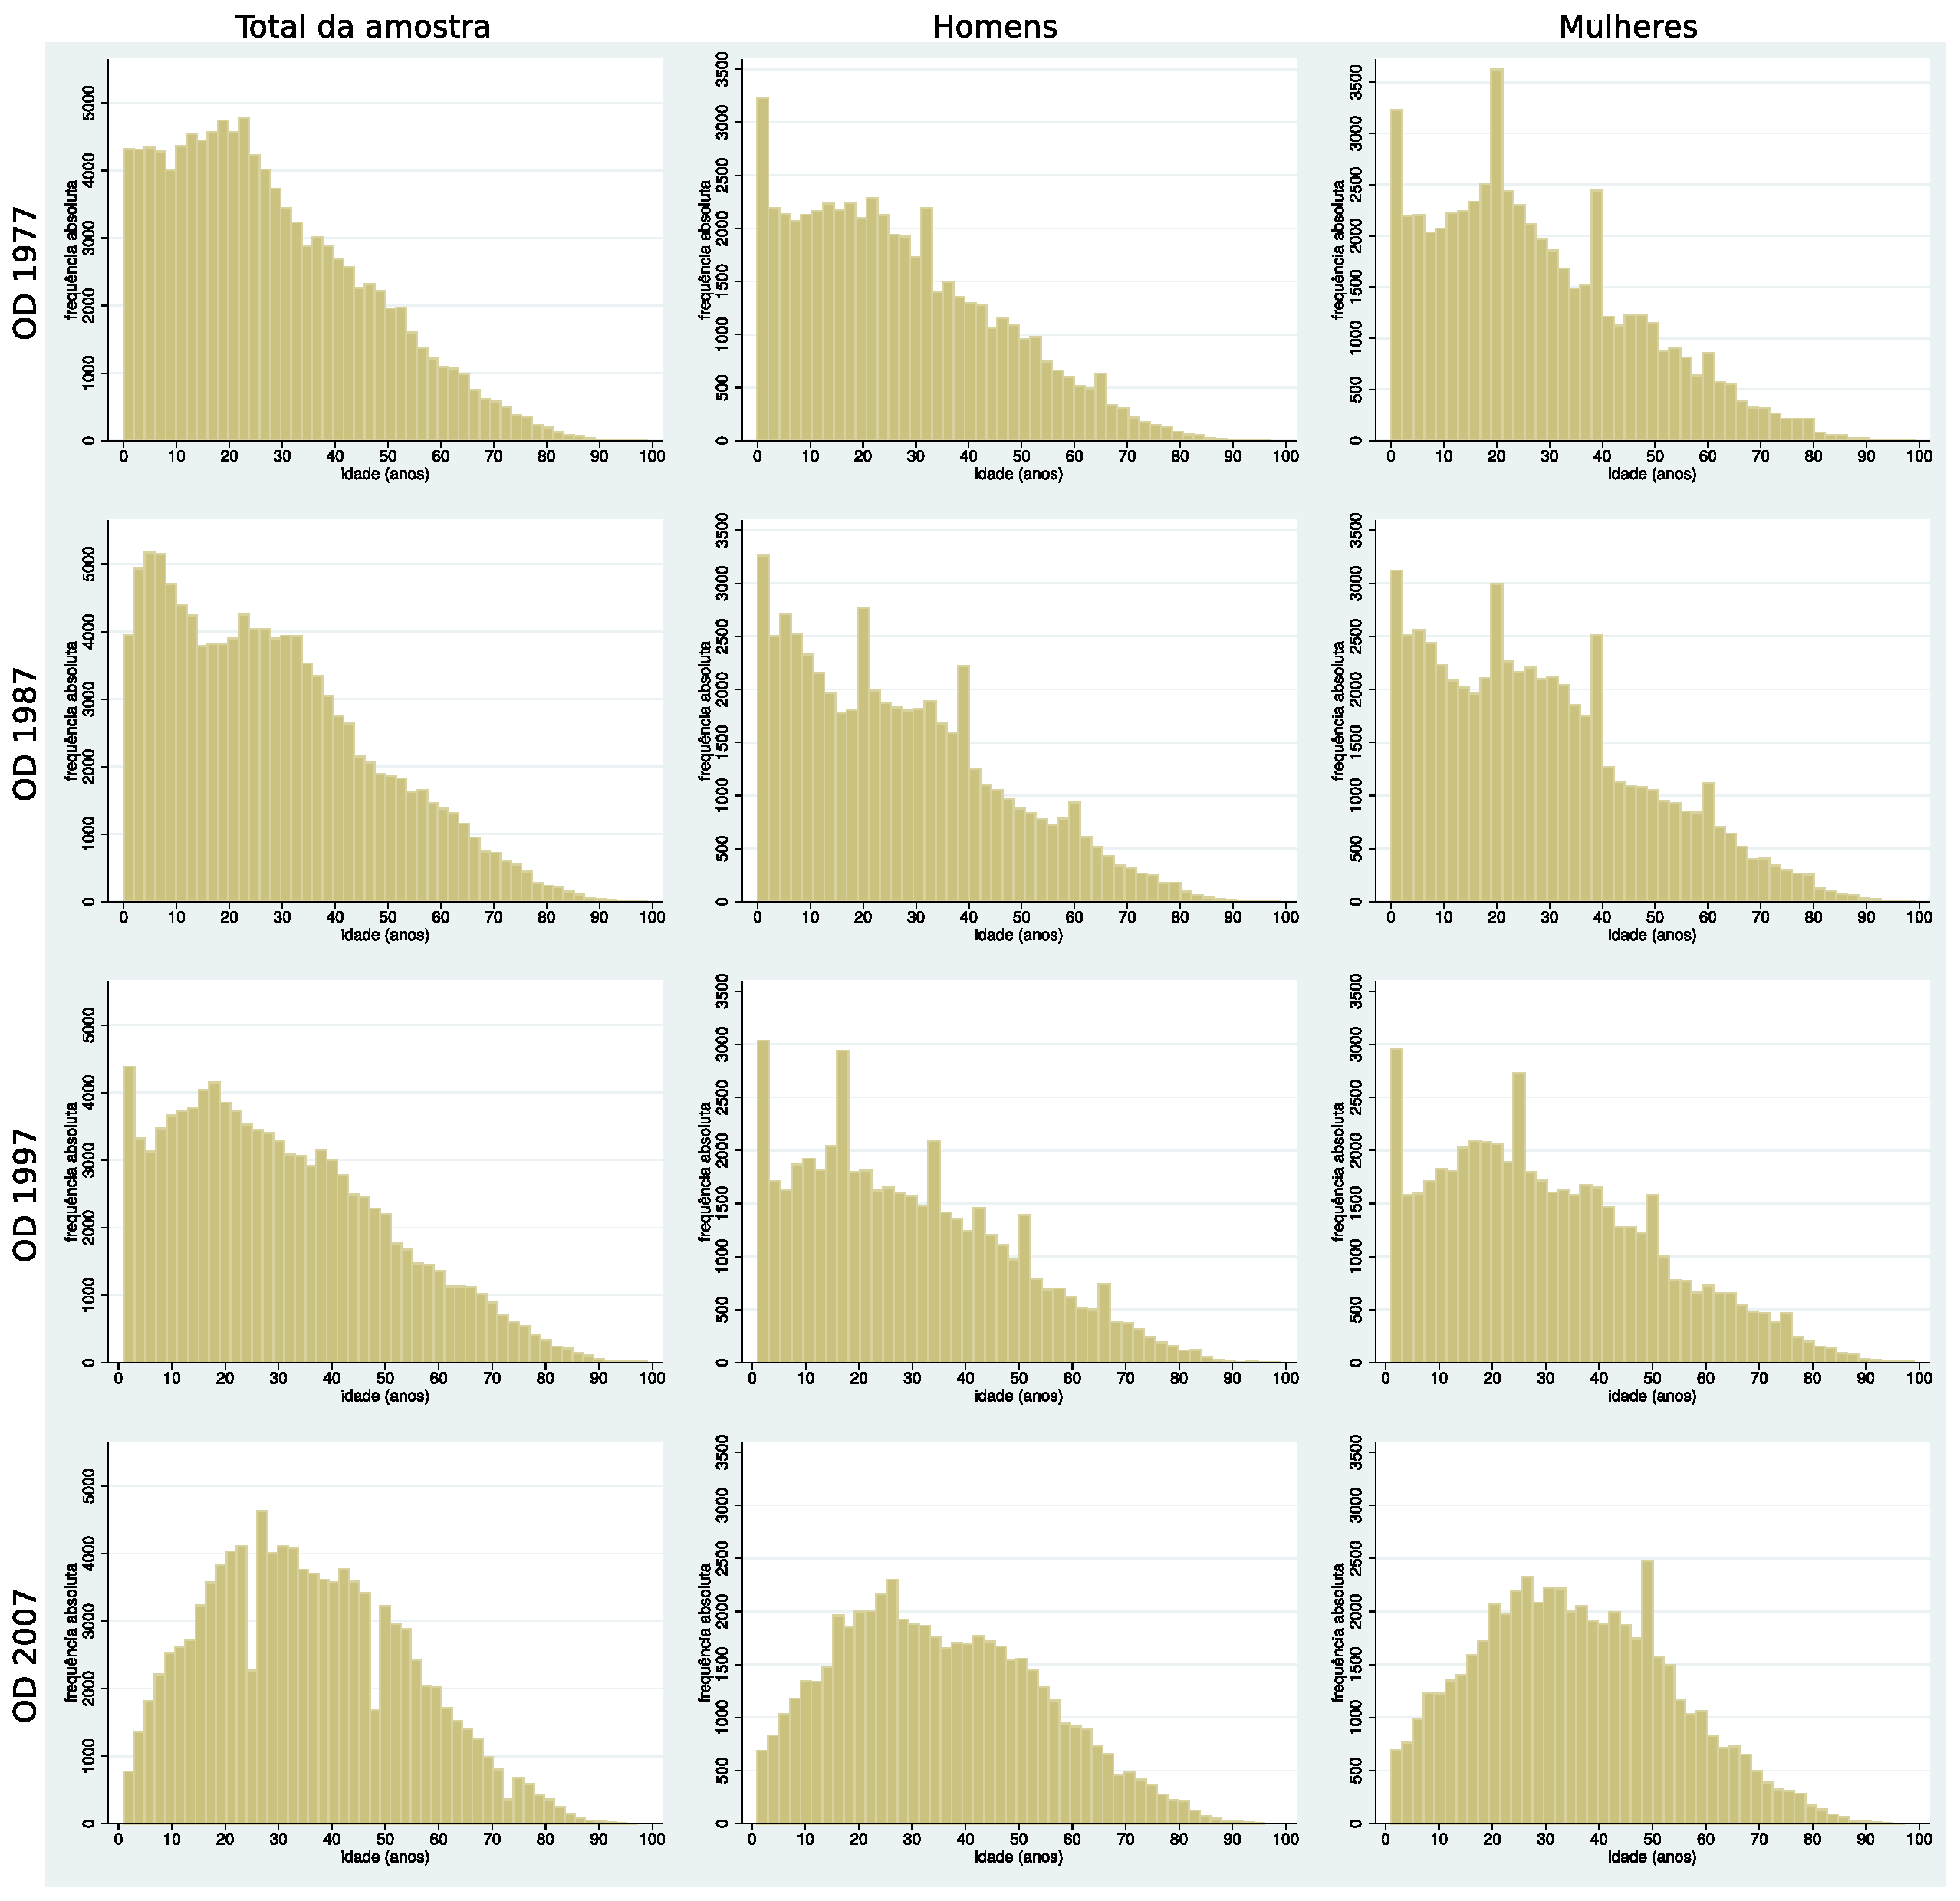
\includegraphics[width=1\textwidth]{./imagens/idade2.eps}%
    \end{center}%
    \fonte{Compilação própria}
\end{grafico}%

\clearpage
No Gráfico \ref{graf:distr-sit-fam} nota-se que para as mulheres houve uma mudança ao longo dessas três décadas. Em 1977, era mais frequente elas ocuparem a posição de filhas (41,81\%), em seguida de cônjuges (36,27\%). A posição de ``pessoa responsável'' pela família é a quarta categoria mais frequente (6,32\%), de seis. Tal distribuição permanace semelhante em 1987. Em 1997, no entanto, a posição de ``pessoa responsável'' pela família (11,13\%) já quase se equipara à posição de ``outro parente/agregado(a)'' (11,27\%). Em 2007, já é quase um quarto das mulheres entrevistadas que são responsáveis por suas famílias (24,21\%), representando aumento de quase 4 vezes em relação aos perecentuais de 1977. O percentual de mulheres cônjuges/companheiras pouco se altera ao longo do tempo, permanecendo na faixa dos 35\%. Há diminuição da posição de empregado(a) doméstico(a) para ambos sexos, mas a queda é mais acentuada para mulheres (da ordem de 8 vezes entre 1977 e 2007) do que para homens (queda em 2007 para cerca da metade do valor de 1977). Existe, também, queda da frequência daqueles que declaram-se na posição de filho(a) ou enteado(a) tanto para homens como para mulheres - em ordem de grandeza próxima: cerca de 8\% para mulheres e 10\% para homens. Isso pode ser reflexo da diminuição das taxas de fecundidade
\footnote{Por ``taxa de fecundidade total'' entende-se o número médio de filhos que teria uma mulher de uma coorte hipotética (15 e 49 anos de idade) ao final de seu período reprodutivo. Fonte: IBGE. Disponível em: \url{http://www.ibge.gov.br/home/estatistica/populacao/condicaodevida/indicadoresminimos/conceitos.shtm\#tf}} da população (ver Tabela \ref{tab:taxa-fecund}). Entre os homens percebe-se que houve crescimento entre aqueles com posição de ``pessoas responsável'' de cerca de 8\%, e também dos que declaram-se cônjuge/companheiro (cerca de 20 vezes) - esta última constatação é coerente com o fato de mais mulheres serem a principal fonte de renda doméstica, ou seja, a ``pessoa responsável'' da família.

\begin{table}[htb]
    \IBGEtab{%\renewcommand{\arraystretch}{1.5}%%\ABNTEXfontereduzida%
	    \renewcommand{\arraystretch}{1.5}
        \caption{Evolução das taxas de fecundidade no Brasil, de 1970 a 2010}
		\label{tab:taxa-fecund}
    }{%
	    \begin{tabular}{P{5.00cm} P{1.50cm} P{1.50cm} P{1.50cm} P{1.50cm} P{1.50cm}}
            \toprule
	           \headerTabCenterCell{Ano} &
   	           \headerTabCenterCell{1970} &
   	           \headerTabCenterCell{1980} &
   	           \headerTabCenterCell{1991} &
   	           \headerTabCenterCell{2000} &
   	           \headerTabCenterCell{2010} \\
		    \midrule \midrule
				Taxa de fecundidade (Brasil)&
				5,8&
				4,4&
				2,7&
				2,4&
		        1,9\\
			\midrule
				Taxa de fecundidade (Sudeste)&
				4,6&
				3,2&
				2,4&
				2,1&
		        1,7\\
			\midrule
				Taxa de fecundidade (São Paulo)&
				3,94&
				3,24&
				2,28&
				2,05&
		        1,67\\
			\bottomrule	
		\end{tabular}
    }{%
		\fonte{Compilação a partir de dados dos censos do IBGE disponíveis em \url{http://seculoxx.ibge.gov.br/populacionais-sociais-politicas-e-culturais/busca-por-palavra-chave/populacao/810-fecundidade} Acesso em 17 de novembro de 2014}
		\nota{Ao analisar as taxas de fecundidades para as Grandes Regiões, nota-se que o Sudeste tem os menores percentuais de mulheres que tiveram filhos em todos os subgrupos etários.}
		}
\end{table}

É possível que essa transformação dos papeis sociais desempenhados por homens e mulheres dentro do núcleo familiar ao longo das últimas décadas altere de maneira significativa os padrões de mobilidade de ambos grupos.

\clearpage

\begin{grafico}[htb]%
    \caption{\label{graf:distr-sit-fam}Distribuição da situação familiar de respondentes das Pesquisas OD 1977, 1987, 1997 e 2007, por sexo}%
    \begin{center}%
        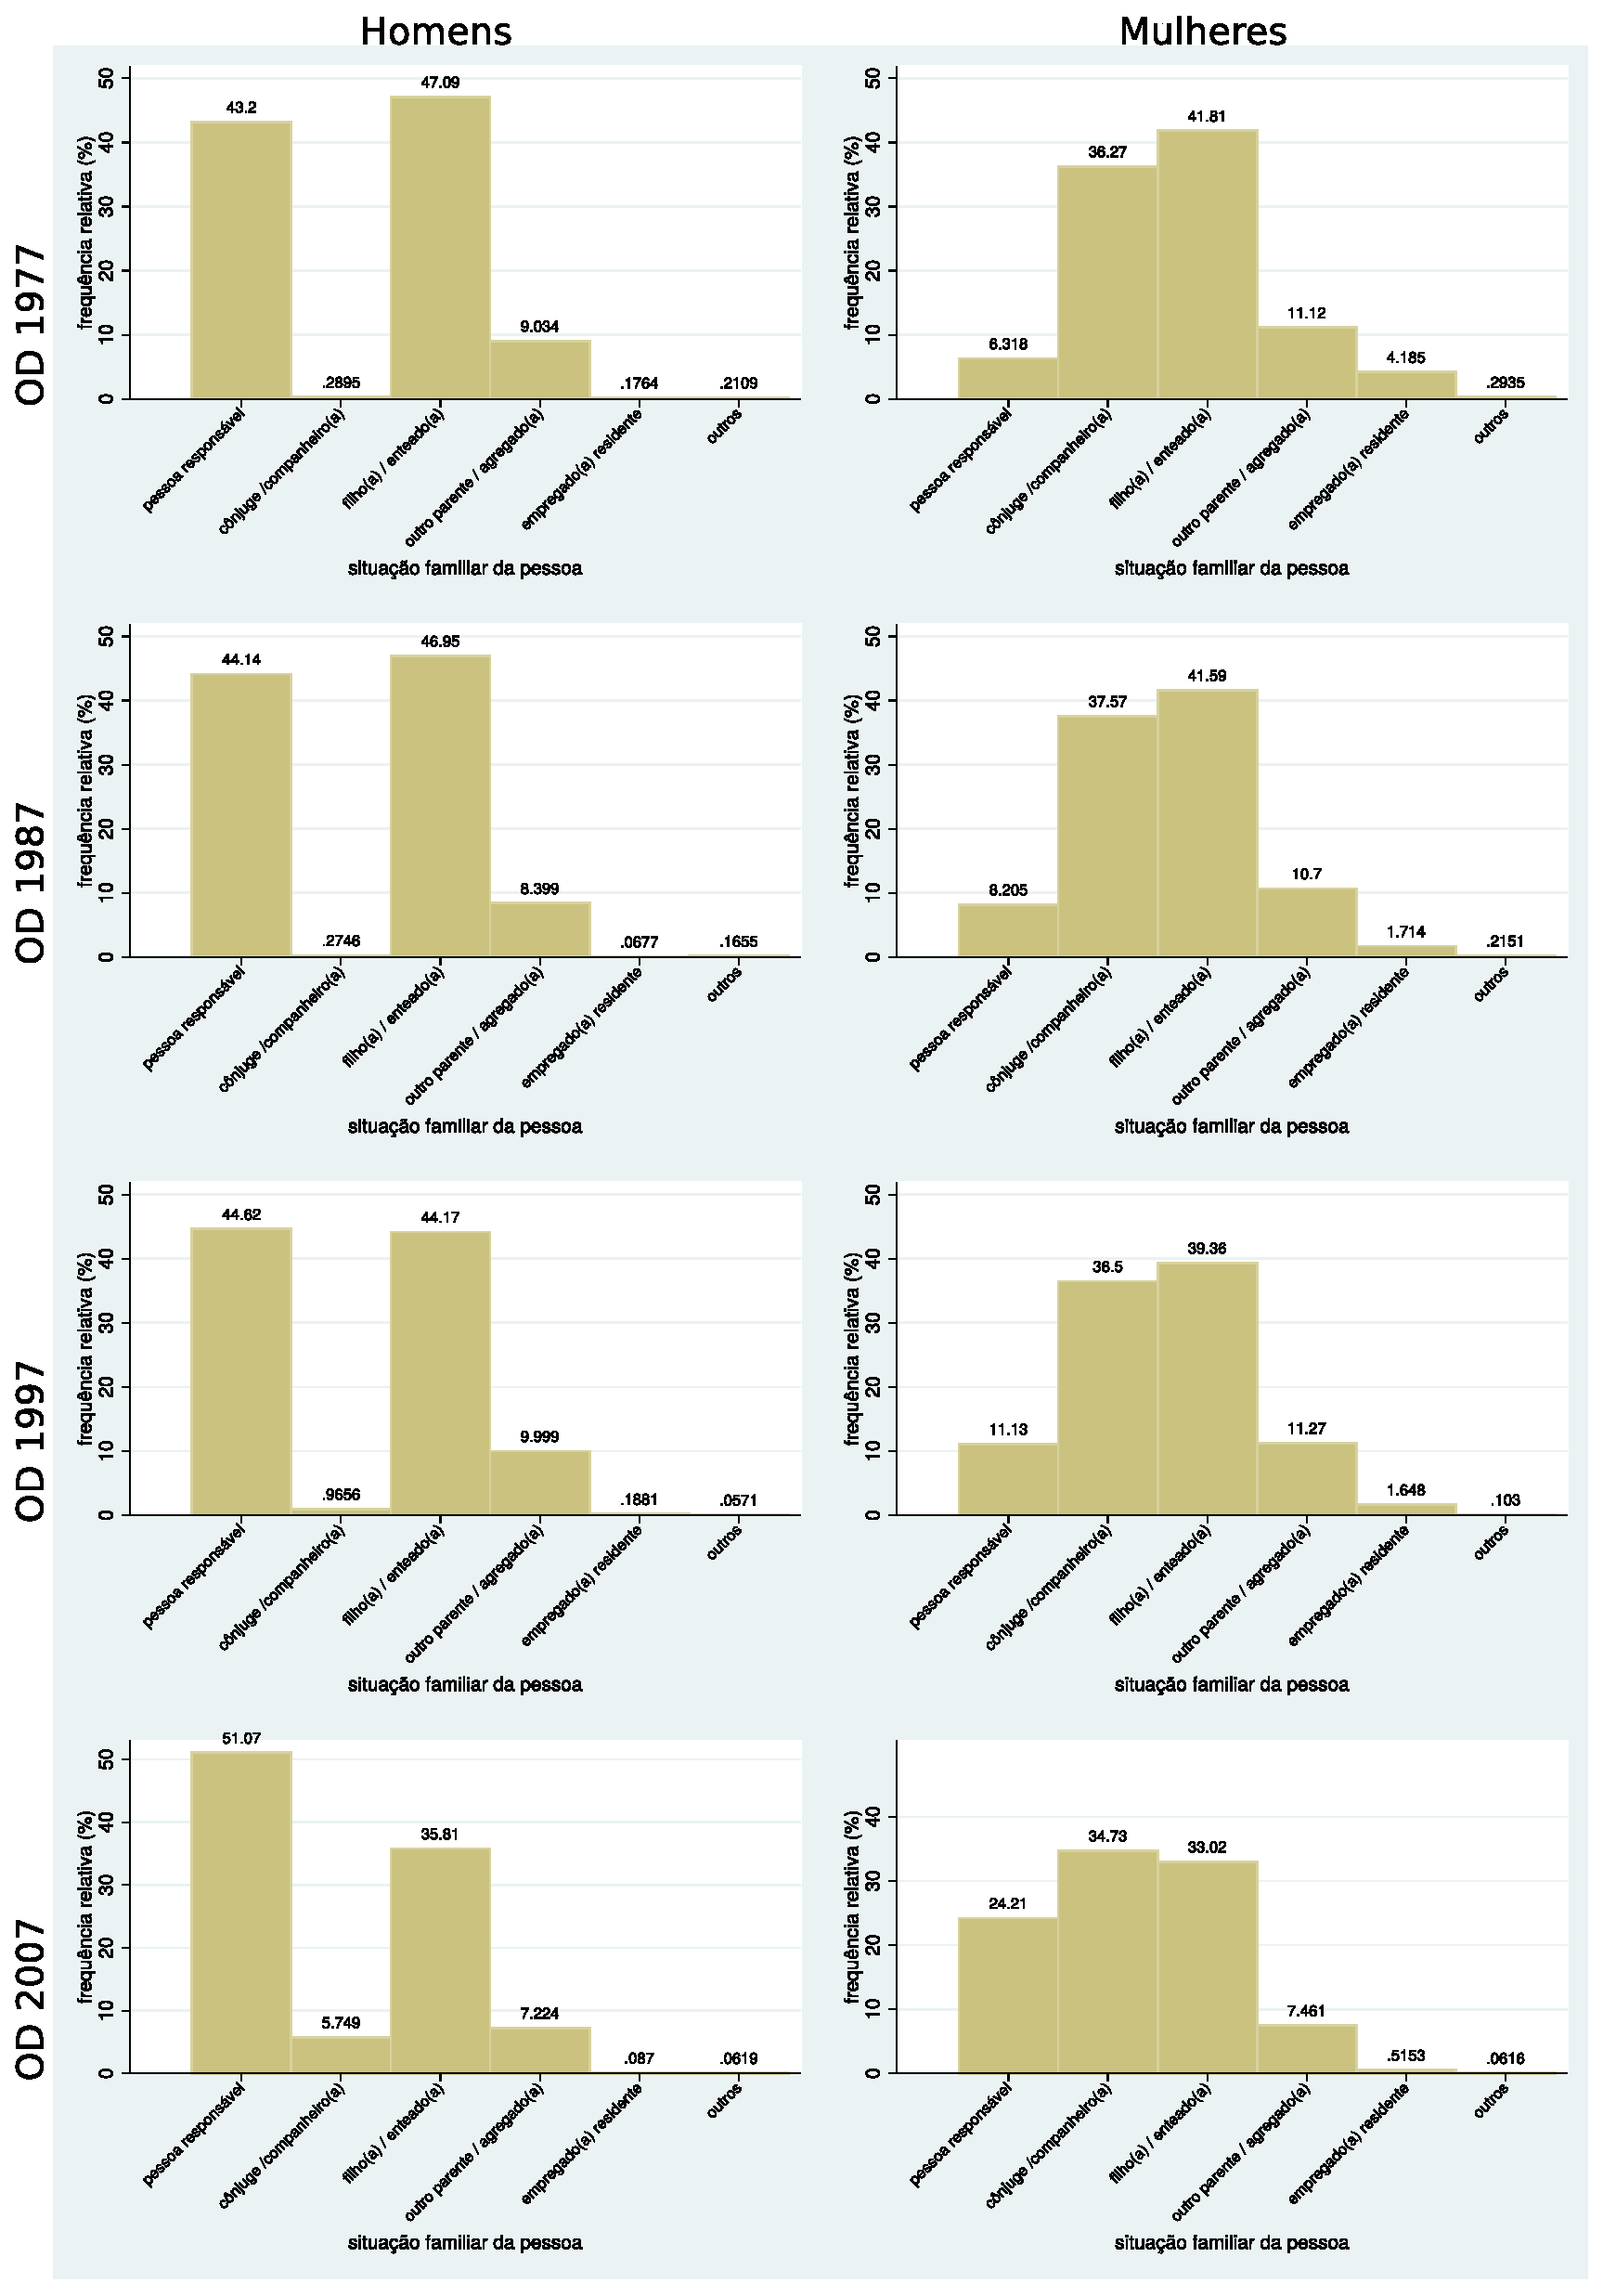
\includegraphics[width=1\textwidth]{./imagens/sitfam2.eps}%
    \end{center}%
    \fonte{Compilação própria}
\end{grafico}%

\clearpage

No Gráfico \ref{graf:distr-grau-instr} nota-se que em 1977 tanto homens como mulheres dispunham de pouco tempo de escolaridade - cerca de três quartos da população ou era analfabeta ou possuía no máximo o fundamental incompleto. Nessa época, nos três níveis de instrução superiores a esse os homens tinham índices maiores que as mulheres. O grau de instrução da população vai aumentando e em 1987, o grau de escolarização feminino é levemente superior ao masculino nas categorias ``fundamental completo / médio incompleto'' e ``médio completo / superior incompleto''. Na categoria ``superior completo'' o grau de instrução masculino é um pouco superior, situação que se inverte em 2007. Neste último ano de análise, as mulheres apresentam maiores percentuais nos dois níveis de maior grau de instrução e os homens, nos dois níveis de menor grau de instrução. Mesmo assim, as marcas para ambos são bastante semelhantes e indicam esforços de políticas públicas no sentido de universalizar os Ensinos Fundamental e Médio no Brasil \ref{tab:grau-instr-ef-em}.

\begin{table}[htb]
    \IBGEtab{%\renewcommand{\arraystretch}{1.5}%%\ABNTEXfontereduzida%
	    \renewcommand{\arraystretch}{1.5}
        \caption{Crescimento de matrículas no Ensino Fundamental e Ensino Médio, no Brasil, entre 1975 e 2005}
		\label{tab:grau-instr-ef-em}
    }{%
	    \begin{tabular}{P{2.00cm} P{4.00cm} P{4.00cm}}
            \toprule
	           \headerTabCenterCell{Ano} &
   	           \headerTabCenterCell{Matrículas no Ensino Fundamental} &
   	           \headerTabCenterCell{Matrículas no Ensino Médio}\\
		    \midrule \midrule
				1975&
		    	100*&
				100*\\
			\midrule
				1980&
				115,6&
		        113,1\\
			\midrule
				1990&
				141,0**&
		        180,8\\
			\midrule
				1996&
				169,5&
		        296,4\\
			\midrule
				2000&
				182,7&
		        423,2\\
			\midrule
				2005&
				171,5&
		        466,5\\
			\bottomrule	
		\end{tabular}
    }{%
		\fonte{Adaptado de \citeauthoronline{OLIVEIRA2007} (\citeyear{OLIVEIRA2007})}
		\nota{* Tomou-se por referência o ano de 1975 (1975=100). 
		** O valor refere-se ao ano de 1989.}
	}
\end{table}

O grau de instrução ter se elevado entre 1977 e 2007 influencia não apenas a empregabilidade e, eventualmente as viagens motivo trabalho. O principal impacto esperado desse fenômeno dá-se nas viagens motivo escola - realizadas por um contingente de pessoas cada vez maior, mais diverso e contendo mais faixas etárias.

\begin{grafico}[htb]%
    \caption{\label{graf:distr-grau-instr} Distribuição do grau de instrução de respondentes das Pesquisas OD 1977, 1987, 1997 e 2007, por sexo}%
    \begin{center}%
        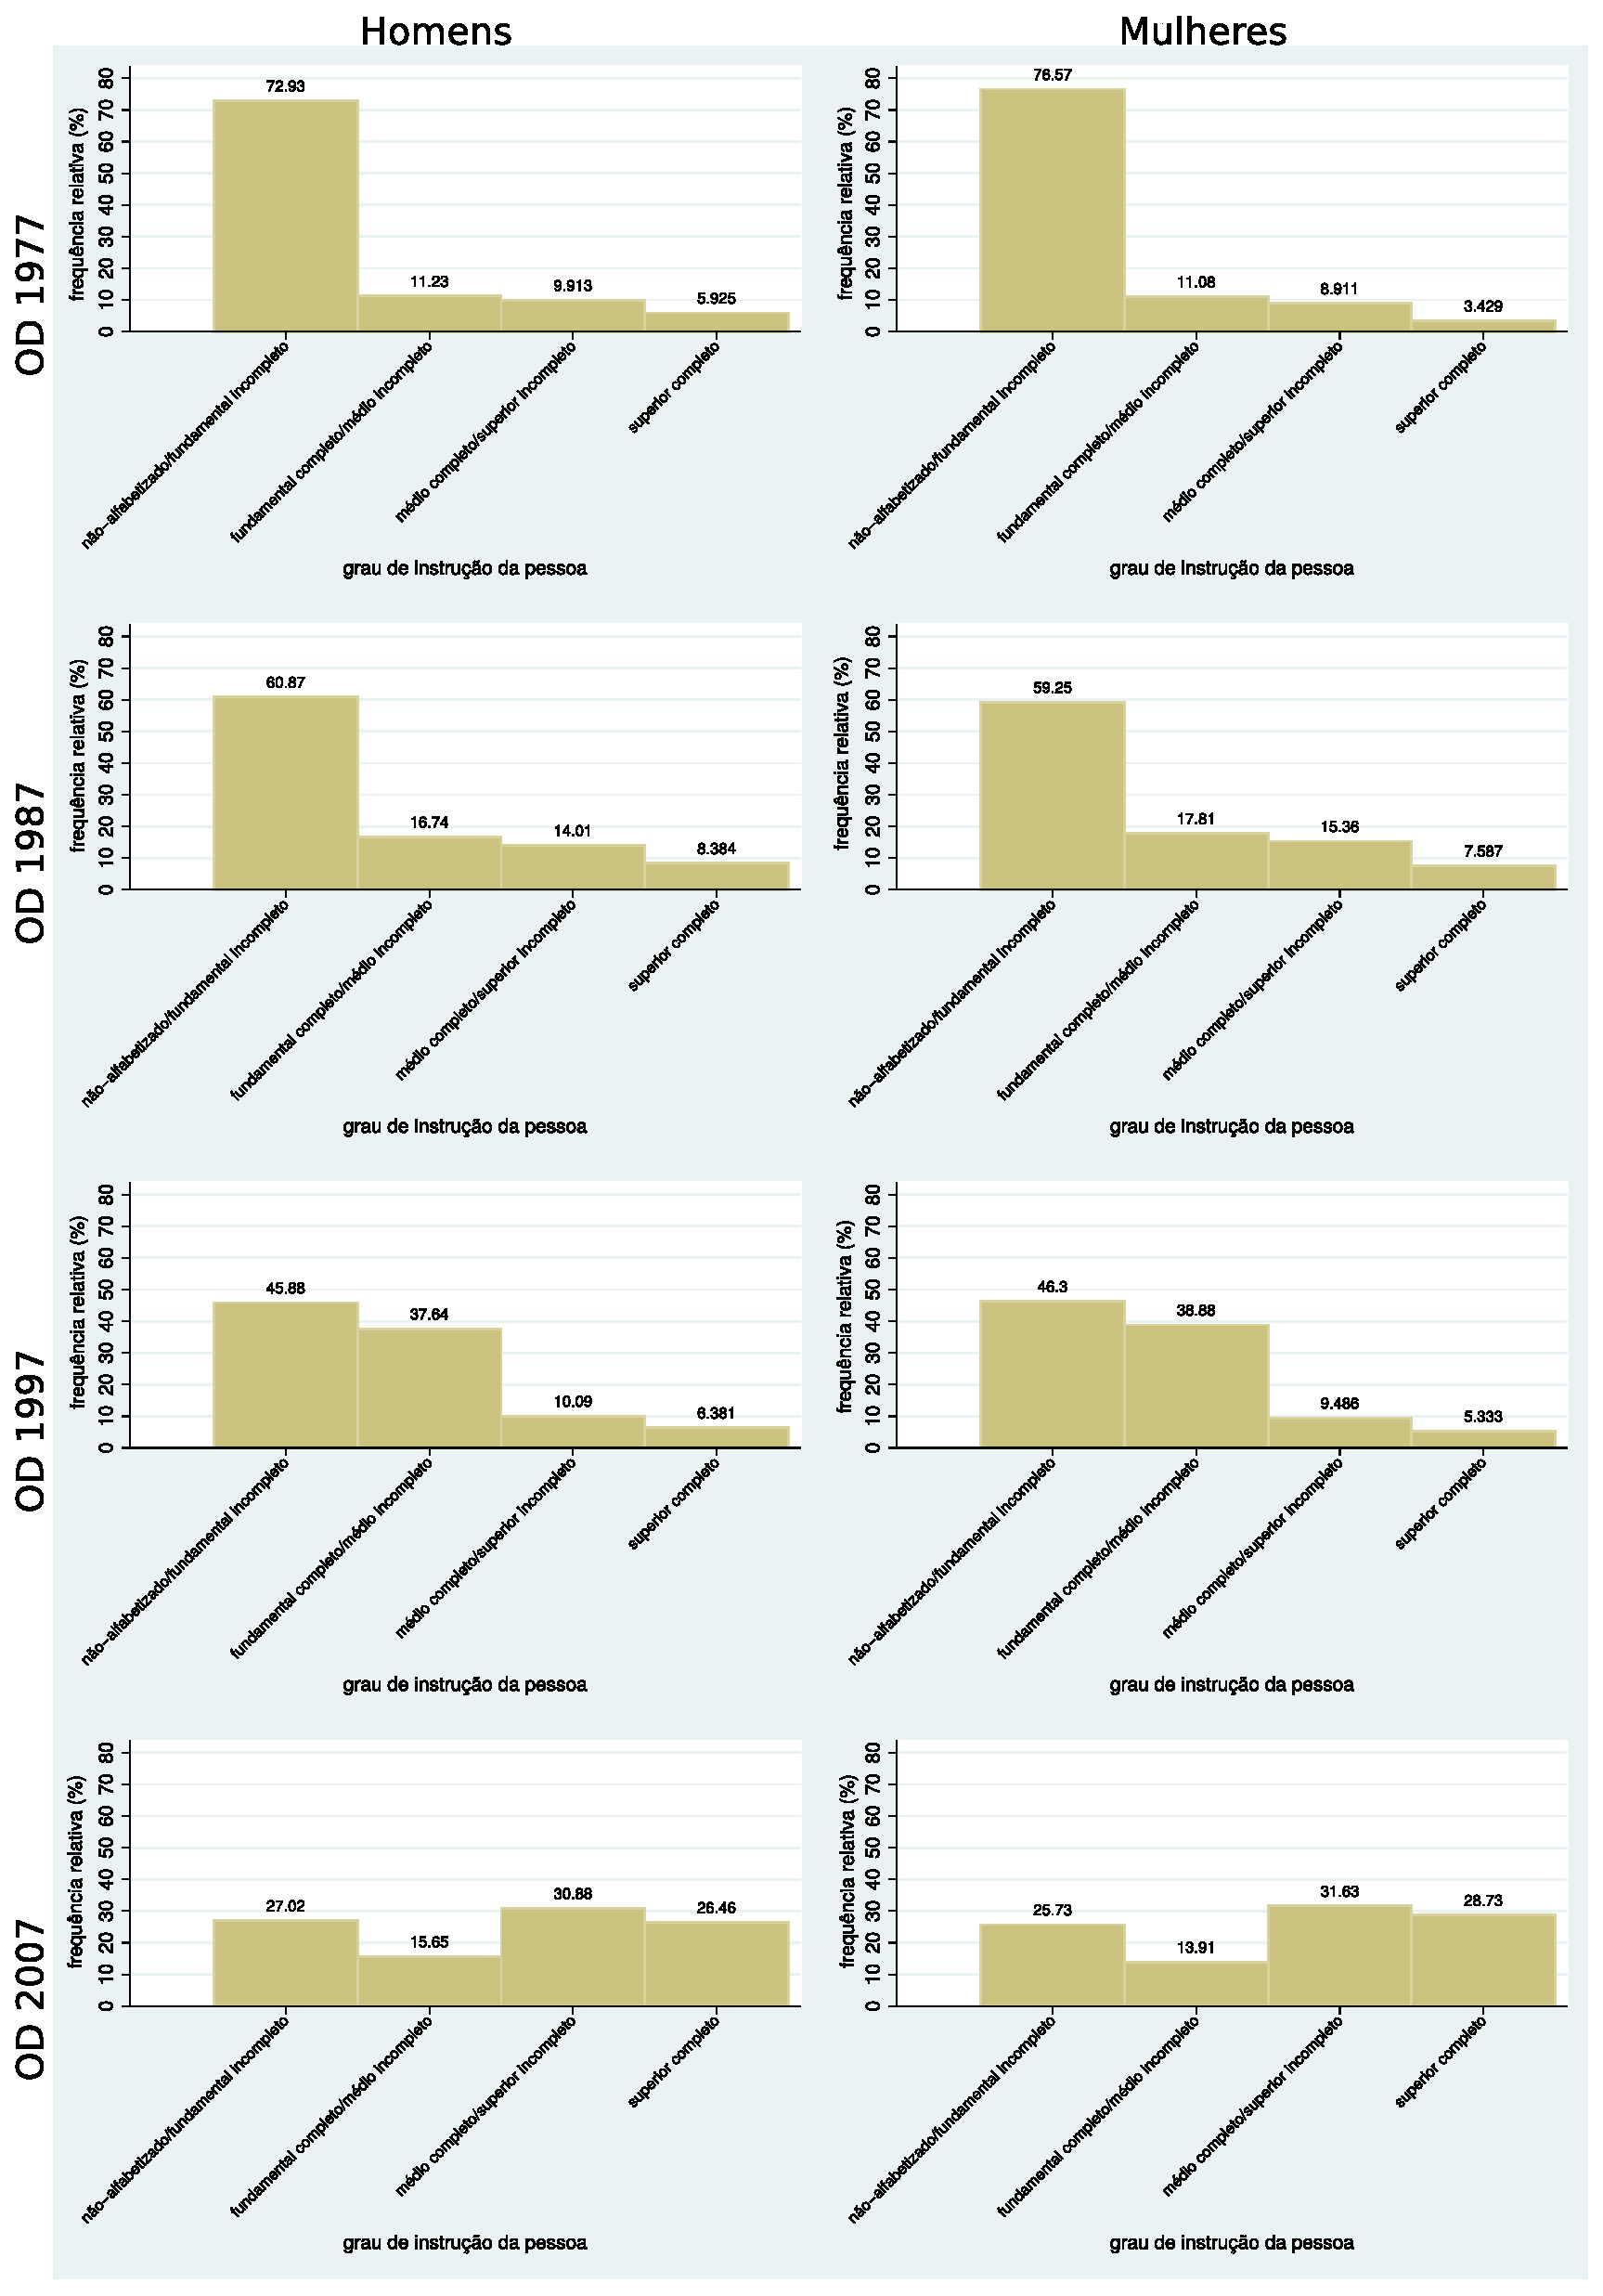
\includegraphics[width=1\textwidth]{./imagens/grauinstr2.eps}%
    \end{center}%
    \fonte{Compilação própria}
\end{grafico}%

\clearpage
Para atribuição da renda foram feitas regressões baseadas nos bens de consumo levantados.
Em 1977, foi adotado o critério \hl{XXX} e a equação \eqref{eq:reg-renda-77} explicita como foi feita a atribuição da renda.
Em 1987, foi adotado o critério ABA/ABIMEPE e a equação \eqref{eq:reg-renda-87} explicita como foi feita a atribuição da renda. 
Em 1997, foi adotado o critério ABIMEPE e a equação \eqref{eq:reg-renda-97} explicita como foi feita a atribuição da renda.
Em 2007, foi adotado o critério ABEP e a equação \eqref{eq:reg-renda-07} explicita como foi feita a atribuição da renda.

\hl{explicar como foi feito o cálculo da renda atribuída, para cada OD}

\hl{explicar como foram trazidos os valores para o valor presente (outubro de 2007)}

\hl{fazer essas transformações no banco e rodar análises f(rend\_ind) e f(renda\_fam)}

\clearpage
Este grupo de análises que se segue busca compreender como essa amostra se comporta em termo de viagens realizadas, em cada ano e diferencialmente entre os anos, olhando para tanto variáveis como duração das viagens e número de viagens realizadas.

%Dentro deste segundo grupo de análises foi de interese buscar verificiar se a variável explicativa sexo era relevante para explicar tanto a duração como o número de viagens. Para tanto foram feitas regressões lineares simples e seus resultados são apresentados na Seção \ref{sec:analises-preliminares}. Também há interesse em verificar se existe alguma diferença estatisticamente significativa nos padrões de deslocamento entre os sexos, para cada \emph{cross-section}. Isso foi feito feito tomando como hipótese nula que as médias de ambos sexos eram iguais, para as variáveis dependentes analisadas. Essa hipótese foi testada e os resultados também são apresentados na Seção \ref{sec:analises-preliminares}.

O Gráfico \ref{graf:distr-dur-viag} foi construído considerando-se apenas as vigens cuja duração fosse igual ou superior a 5 minutos. Em todos anos, para homens e para mulheres, percebem-se alguns picos que ocorrem nos valores múltiplos de cinco minutos. Isso porque a duração expressa trata-se da duração de viagem percebida e declarada pelo(a) respondente. Em 1977, a duração das viagens mais curtas (como 5 e 30 minutos) era menos frequente entre as mulheres (13\% e 14\%, respectivamente) do que entre os homenso (26\% e 15\%). No mesmo ano, as viagens mais longas eram mais frequentes entre as mulheres (5\% para 60 minutos e 2\% para 90 minutos) do que entre os homens (6,5\% para 60 minutos e 3\% para 90 minutos). De 1987 as viagens de 5 minutos passam a ser mais frequentes entre mulheres (32\%) do que entre homens (26,5\%). Essa sitação se inverte em 1997 e retorna em 2007.
Em todas anos as viagens mais longas (de 60 e 90 minutos) São mais frequentes entre os homens do que entre as mulheres.
Na Tabela \ref{tab:dur-med-viag} são apresentadas as durações médias de viagens para homens e mulheres. As médias de homens são superiores às das mulheres, ao nível de significância estatística de 5\%. É possível perceber que a duração média de viagem para ambos vem crescendo e a diferença entre esses grupos vem diminuindo.

\hl{verificar se é preiso apresentar os resultados de teste F e teste t p/ comparação de médias OU ANOVA com prévia averiguaçaõ de matrizes de covariância + teste Levene + teste normalidade (não vai passar...)}

\begin{table}[htb]
    \IBGEtab{%\renewcommand{\arraystretch}{1.5}%%\ABNTEXfontereduzida%
	    \renewcommand{\arraystretch}{1.5}
        \caption{Duração média de viagem, por sexo, por ano}
		\label{tab:dur-med-viag}
    }{%
	    \begin{tabular}{P{1.50cm} P{2.00cm} P{2.00cm} P{3.00cm} P{3.00cm} P{3.00cm}}
            \toprule
	           \headerCenterCell{Ano} &
   	           \headerCenterCell{Duração Média de Viagem para Mulheres (min)} &
   	           \headerCenterCell{Duração Média de Viagem para Homens (min)} &
   	           \headerCenterCell{Desvio Padrão da Duração Média de Viagem para Mulheres} &   	           
   	           \headerCenterCell{Desvio Padrão da Duração Média de Viagem para Homens} &   	           
   	           \headerCenterCell{Diferença entre as durações médias (Dur\_mulher - Dur\_homem)}\\
		    \midrule \midrule
				1977&
		    	29,23&
		    	33,27&
		    	28,52&
		    	31,69&
				-4,04\\
			\midrule
				1987&
				30,27&
				35,82&
				29,29&
				33,11&
		        -5,55\\
			\midrule
				1997&
				32,09&
				35,61&
				30,83&
				33,90&
		        -3,52\\
			\midrule
				2007&
				35,35&
				37,39&
				32,76&
				33,87&
		        -2,04\\
			\bottomrule	
		\end{tabular}
    }{%
		\fonte{Elaboração própria}
	}
\end{table}

Ao fazer a regressão linear da variável duração (valores superiores a 5 minutos) unicamente em função da variável explicativo sexo, para todos anos os p-valores foram inferiores a 0,05, o que mostra indícios de que a variável sexo é umas das variáveis de análise para explicar o tempo dispendido nos deslocamentos.

\begin{grafico}[htb]%
    \caption{\label{graf:distr-dur-viag}Distribuição da duração de viagens de respondentes das Pesquisas OD 1977, 1987, 1997 e 2007, por sexo}%
    \begin{center}%
        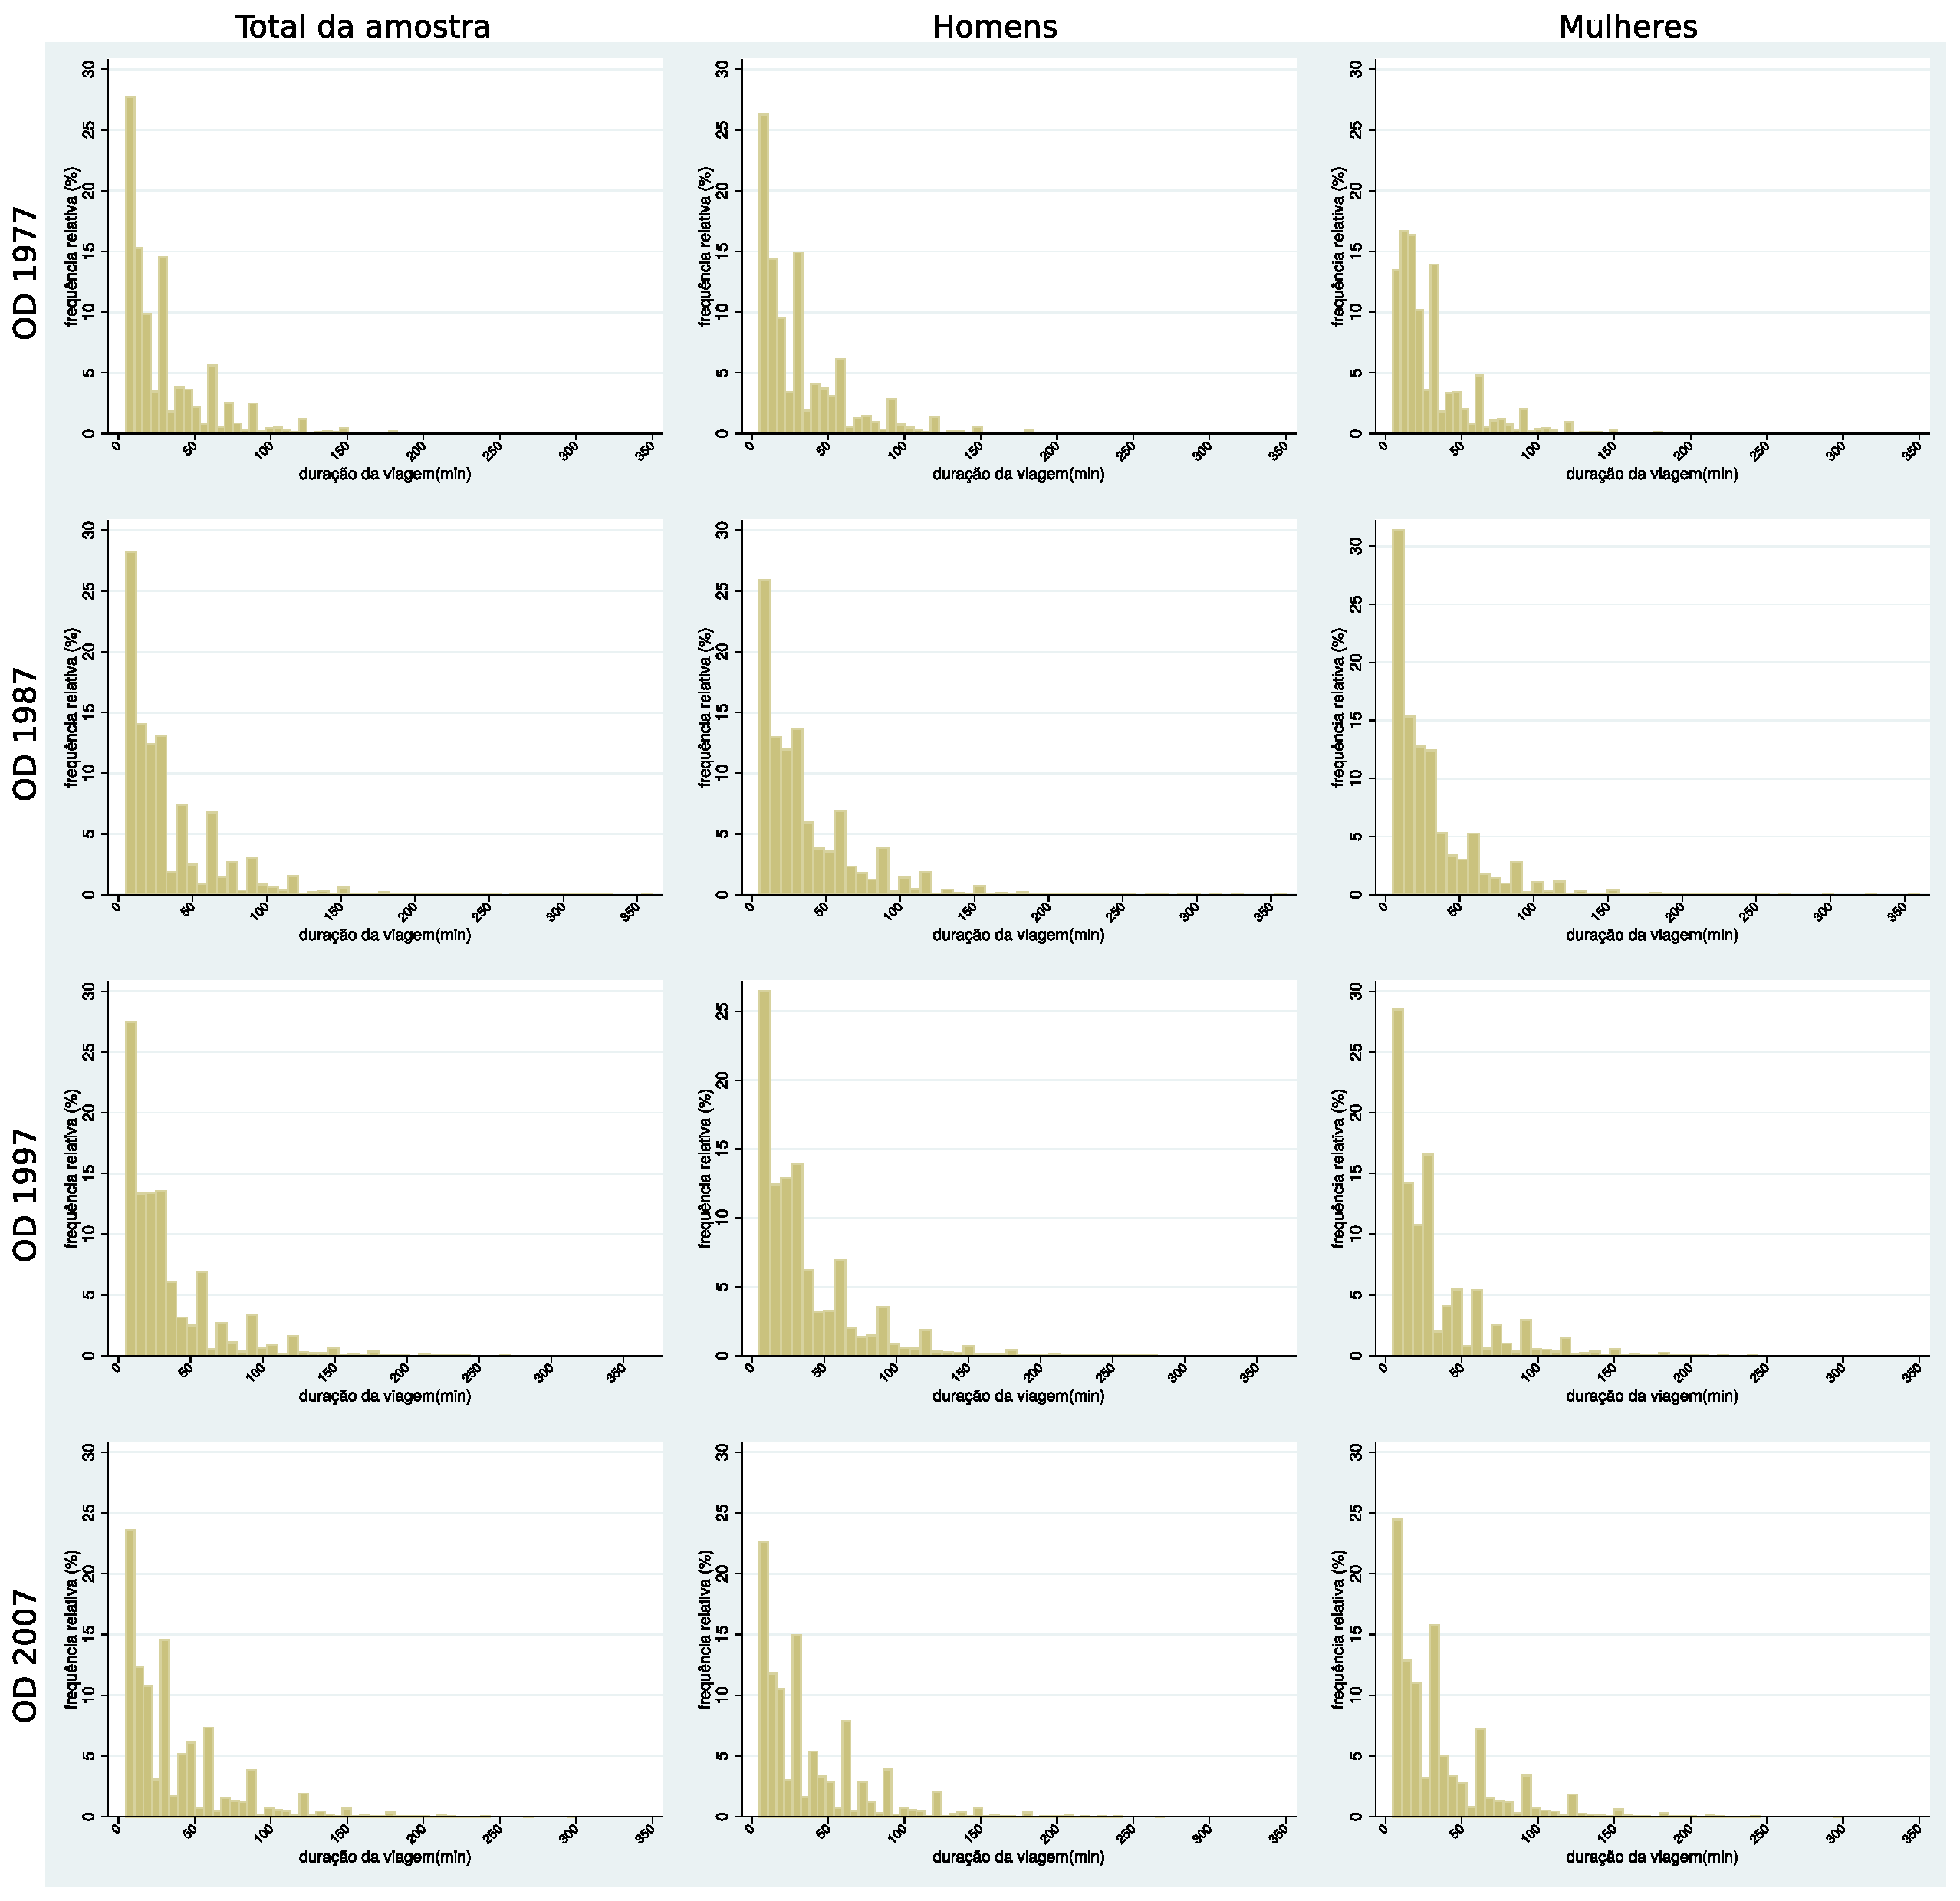
\includegraphics[width=1.1\textwidth]{./imagens/duradeviagens2.eps}%
    \end{center}%
    \fonte{Compilação própria}
\end{grafico}%

\clearpage
Analisando a dsitribuição do número de viagens por pessoa, conforme já era de se esperar, para quem faz viagem (número de viagem é não nulo) existe a predominância do valor 2, o que indica que é caracaterístico de pessoas que trabalham ou que estudam, pois saem da sua residência com esse propósito (que ocupa a maior parte do seu dia) e depois retornam à residência apśoa atividade. O que vale analisar no Gráfico \ref{graf:distr-num-viag} é a relação entre as viagens nulas (não sai de casa) e as viagens de idae volta (valores iguais a 2). Para homens, o número de viagens nulo é menos frequente que o número de viagens de valor 2 para todos anos de análise. Já para as mulheres, em 1977 as viagens nulas eram a maioria, indicando certa fixitude delas. Essa porcentagem vai diminuido e a porcentagem no número de viagens igual a 2 vai crescendo, ficam próximas em 1997 e, em 2007, inverte-se a situação observada em 1977. Coincidentemente com a conquista de maior participação no mercado de trabalho, essa alteração pode ser indícios de que as mulheres ganharam mobilidade, restringindo-se menos ao espaço doméstico.

Na Tabela \ref{tab:num-med-viag} são apresentados os números médios de viagens para homens e mulheres. As médias de homens são superiores às das mulheres, ao nível de significância estatística de 5\%. O número médio de viagens para os homens caiu entre 1977 e 1997, voltando a subir em 2007. \hl{pq??} O número médio de viagens para as mulheres aumntou desde 1977 até 2007. Apesar dessa mudança de tendência no padrão masculino, a diferença entre os gêneros só tem diminuido.

Ao fazer a regressão linear da variável total de viagens da pessoa (para o primeiro registro da pessoa) unicamente em função da variável explicativo sexo, para todos anos os p-valores foram inferiores a 0,05, o que mostra indícios de que a variável sexo é umas das variáveis de análise para explicar a quantidade de viagens feitas pelo indivíduo.

%\hl{verificar se é preciso apresentar os resultados de teste F e teste t p/ comparação de médias OU ANOVA com prévia averiguaçaõ de matrizes de covariância + teste Levene + teste normalidade (não vai passar...)}

\begin{table}[htb]
    \IBGEtab{%\renewcommand{\arraystretch}{1.5}%%\ABNTEXfontereduzida%
	    \renewcommand{\arraystretch}{1.5}
        \caption{Número médio de viagens, por sexo, por ano}
		\label{tab:num-med-viag}
    }{%
	    \begin{tabular}{P{1.00cm} P{2.00cm} P{2.00cm} P{3.00cm} P{3.00cm} P{3.50cm}}
            \toprule
	           \headerCenterCell{Ano} &
   	           \headerCenterCell{Número Médio de Viagem para Mulheres (min)} &
   	           \headerCenterCell{Número Médio de Viagem para Homens (min)} &
   	           \headerCenterCell{Desvio Padrão da Número Médio de Viagem para Mulheres} &   	           
   	           \headerCenterCell{Desvio Padrão do Número Médio de Viagem para Homens} &   	           
   	           \headerCenterCell{Diferença entre os números médios de viagens (Nº\_viag\_mulher - Nº\_viag\_homem)}\\
		    \midrule \midrule
				1977&
		    	1,40&
		    	2,09&
		    	1,64&
		    	1,92&
				-0,69\\
			\midrule
				1987&
				1,42&
				1,89&
				1,59&
				1,61&
		        -0,47\\
			\midrule
				1997&
				1,53&
				1,79&
				1,63&
				1,60&
		        -0,26\\
			\midrule
				2007&
				1,75&
				1,98&
				1,64&
				1,58&
		        -0,23\\
			\bottomrule	
		\end{tabular}
    }{%
		\fonte{Elaboração própria}
	}
\end{table}


\begin{grafico}[htb]%
    \caption{\label{graf:distr-num-viag}Distribuição do número de viagens por respondente das Pesquisas OD 1977, 1987, 1997 e 2007, por sexo}%
    \begin{center}%
        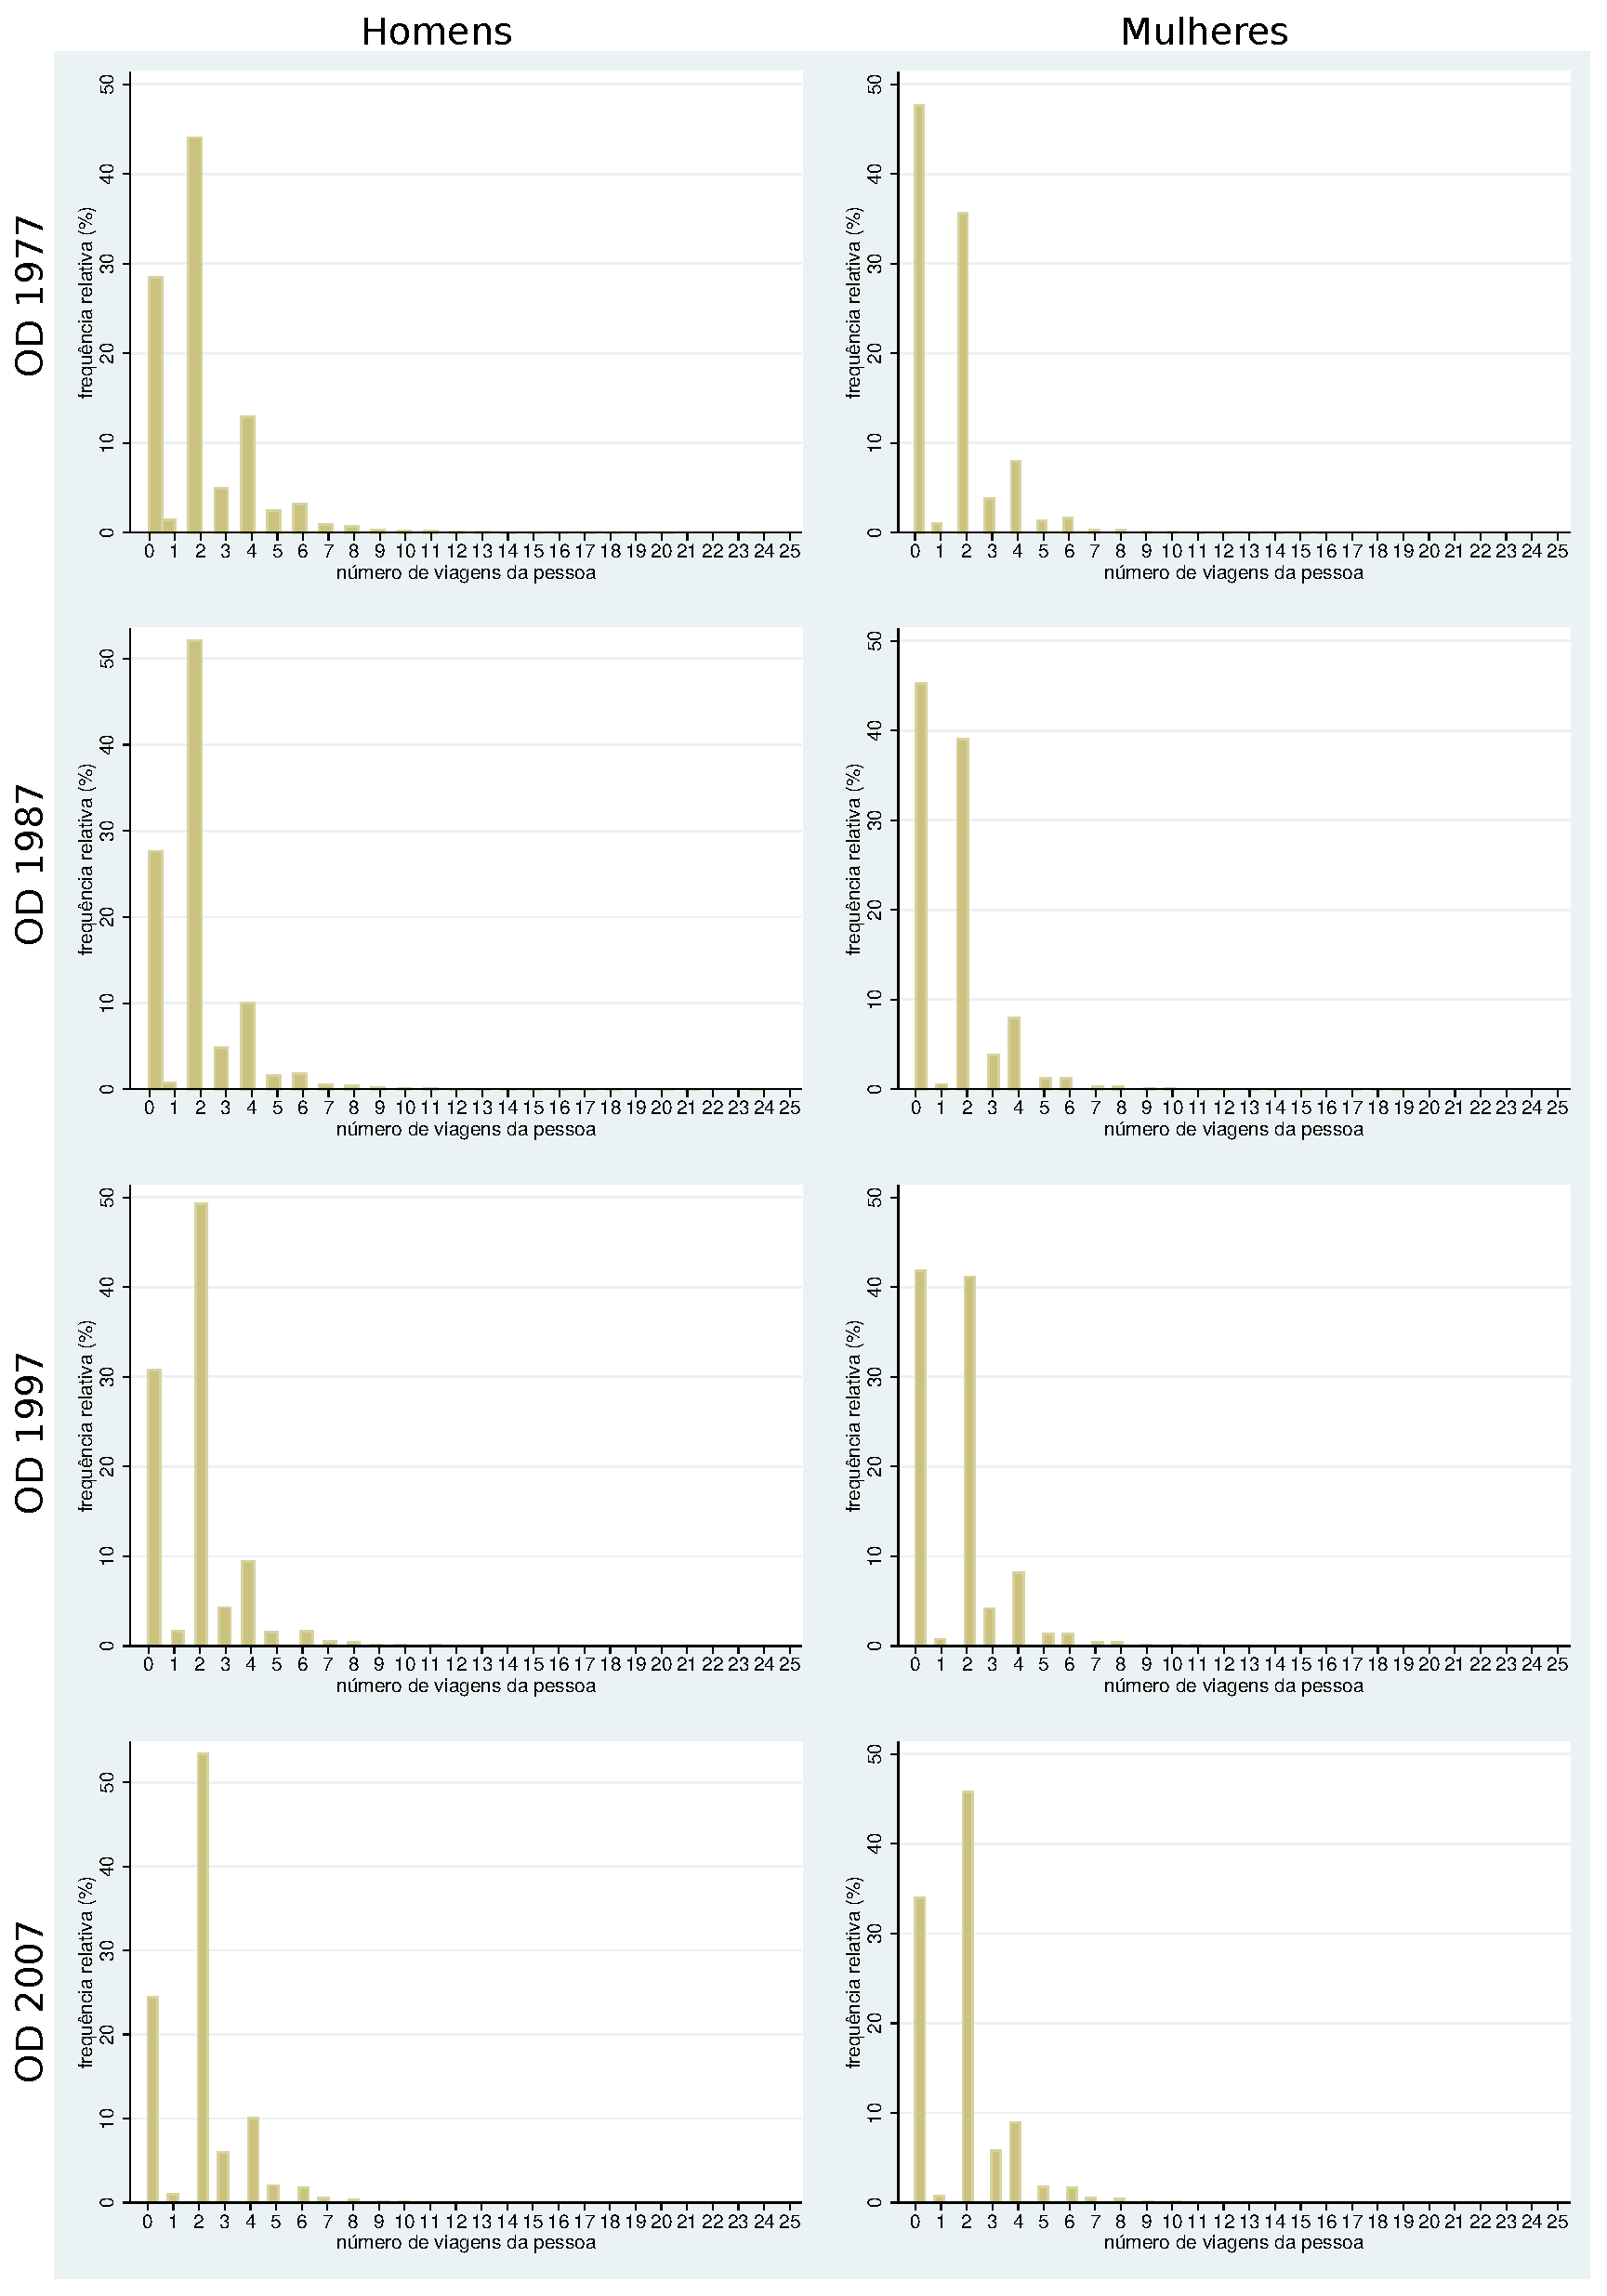
\includegraphics[width=1\textwidth]{./imagens/qtdeviagens2.eps}%
    \end{center}%
    \fonte{Compilação própria}
\end{grafico}%


% ----------------------------------------------------------
% Capitulo de Conclusões e Próximos Passos
% ---
% ---
% Capitulo Considerações Finais
% ---
\chapter{Algumas Considerações e Próximos Passos}\label{chap:considfinais}
% META: 5p.

Cheguei até aqui!!! UHU!!!


A divisão do trabalho de acordo com o gênero implica diferentes padrões de atividades e, assim, diferentes padrões de viagens. As mulheres desempenham diferentes papéis no mercado de trabalho e também na família, elas têm conseguido diminuir as desigualdades no mercado de trabalho ao longo do tempo mas não vêm obtendo o mesmo êxito em relação ao trabalho doméstico. A existência de filhos também influencia marcadamente o padrão de atividades da família e principalmente da mulher, principal responsável por seus cuidados. A sobrecarga do trabalho doméstico ser deixada para o lado feminino da família implica menos disponibilidade de tempo para as mulheres e resulta numa maior pressão por utilização de modos de transportes que ofereçam mais velocidade e flexibilidade de itinerário, ou seja, um incentivo ao uso do carro. Consequentemente, as mulheres que possuem filhos são as que apresentam a maior restrição de mobilidade.

Logo, tendo em vista a elaboração de políticas de transporte público que o torne mais atrativo para as mulheres, é preciso primeiramente garantir que o transporte público seja acessível. Isto significa tanto não haver barreiras econômicas (tarifárias), já que mulheres têm rendimento médio inferior a homens, quanto haver capilaridade suficiente da rede, para que haja a percepção de que existe transporte público ``à disposição'', assim como se tem com o carro. Em segundo lugar é preciso que o(s) modo(s) seja adequado à atividade que será desempenhada. Para mulheres, se considerarmos as viagens motivo ``manutenção'' da casa, acompanhar crianças à escola ou ao médico e ir às compras são atividades relevantes. No Reino Unido, Hamilton e Jenkins (2000) apontam para a falta de adequação da infraestrutura de transportes às necessidades socialmente atribuídas às mulheres. No Brasil, o diagnóstico não difere à exceção de poucos municípios como Curitiba: é impossível uma mulher utilizar um ônibus com um carrinho de bebê ou carrinho de compras. 

Por fim, constatando a influência da divisão do trabalho sobre o padrão de mobilidade de acordo com o gênero, podem ser tomadas medidas de incentivo ao uso do transporte público de forma a considerar a diversidade de necessidades que levam as pessoas a se locomoverem nas cidades (GTZ, 2007). São exemplos de medidas que podem ser adotadas: incremento da infra-estrutura do sistema de transporte existente, capilarização da rede, mudança na metodologia de pesquisa origem-destino para que se passe a considerar viagens a pé inferiores a 500m ou trechos a pé na cadeia de viagens. Estas mudanças podem aumentar a eficácia e eficiência do sistema de transporte urbano, já que este será mais atrativo - não apenas para as mulheres - e pode contribuir com a diminuição dos congestionamentos.

Para \hl{Daus (apud FREITAG)} algumas cidades extra-europeias, mesmo com seu vertiginoso crescimento e urbanização, pode servir de exemplo de inovação e capacidade de adaptação.


Conforme pode ser observado no Quadro \ref{qua:cronograma} pretende-se ....


\begin{quadro}[htb]
    \IBGEtab{
        \renewcommand{\arraystretch}{1.5}
        \ABNTEXfontereduzida
        \caption[Cronograma]{\label{qua:cronograma}Cronograma das atividads a serem desenvolvidas no mestrado em 2015}
	}{%
        \begin{tabular}{|p{3.0cm}|P{0.72cm}|P{0.72cm}|P{0.74cm}|P{0.72cm}|P{0.72cm}|P{0.72cm}|P{0.72cm}|P{0.72cm}|P{0.72cm}|P{0.72cm}|}
           \hline
		       \headerCenterCell{Atividade} & 
		       \headerCenterCell{Jan} & 
		       \headerCenterCell{Fev} & 
		       \headerCenterCell{Mar} &
   		       \headerCenterCell{Abr} & 
   		       \headerCenterCell{Mai} & 
   		       \headerCenterCell{Jun} & 
   		       \headerCenterCell{Jul} & 
   		       \headerCenterCell{Ago} & 
   		       \headerCenterCell{Set} & 
   		       \headerCenterCell{Out}\\ 
		    \hline\hline
		        Avanço na revisão da literatura de acordo com sugestões da banca de qualificação&
		        X &
		        X &
		        X &
		        X &
		        X &
		        &
		        &
		        &
		        &
		        \\
		    \hline
		    	Preparação do banco de dados reunindo OD-77, OD-87, OD-97 e OD-07&
		        X &
		        &
		        &
		        &
		        &
		        &
		        &
		        &
		        &
		        \\
		    \hline
		    	Modelagem dos dados em pseudo-painel&
		        X &
		        X &
		        X &
		        &
		        &
		        &
		        &
		        &
		        &
		        \\
		    \hline
		    	Validação do modelo e análise de resultados&
		        &
		        &
		        &
		        X &
		        X &
		        X &
		        &
		        &
		        &
		        \\
		    \hline
		    	Redação da dissertação&
		        X &
		        X &
		        X &
		        X &
		        X &
		        X &
		        X &
		        X &
		        &
		        \\
   		    \hline
		    	Revisão do texto da dissertação&
		        &
		        &
		        &
		        &
		        &
		        &
		        &
		        &
		        X &
		        \\
		    \hline
		    	Defesa da dissertação de mestrado diante banca&
		        &
		        &
		        &
		        &
		        &
		        &
		        &
		        &
		        &
		        X\\
		    \hline
		\end{tabular}
	}{%
		\fonte{\cite{AVRITZER2007}}
    }
\end{quadro}


% ---
% ----------------------------------------------------------
% Finaliza a parte no bookmark do PDF
% para que se inicie o bookmark na raiz
% e adiciona espaço de parte no Sumário
% ----------------------------------------------------------
\phantompart

% ---
% Conclusão (outro exemplo de capítulo sem numeração e presente no sumário)
% ---
%\chapter*[Conclusão]{Conclusão}
%\addcontentsline{toc}{chapter}{Conclusão}
% ---

% ----------------------------------------------------------
% ELEMENTOS PÓS-TEXTUAIS
% ----------------------------------------------------------
\postextual
% ----------------------------------------------------------

% ----------------------------------------------------------
% Referências bibliográficas
% ----------------------------------------------------------
\bibliography{dissertacao}

% ----------------------------------------------------------
% Glossário
% ----------------------------------------------------------
%
% Consulte o manual da classe abntex2 para orientações sobre o glossário.
%
%\glossary

% ----------------------------------------------------------
% Apêndices
% ----------------------------------------------------------

% ---
% Inicia os apêndices
% ---
%\begin{apendicesenv}

% Imprime uma página indicando o início dos apêndices
%\partapendices
% ----------------------------------------------------------
%\include{textos/apendices/apendice}
% ----------------------------------------------------------
%\end{apendicesenv}
% ---


% ----------------------------------------------------------
% Anexos
% ----------------------------------------------------------

% ---
% Inicia os anexos
% ---
\begin{anexosenv}

% Imprime uma página indicando o início dos anexos
\partanexos

% ---
%%%%%%%%%%%%%%%%%%%%%%%%%%%%%%%%%%%%%%%%%%%
%% ---
\chapter{Correspondência entre Zonas das Pesquisas Origem Destino por meio das Unidades de Correspondência entre Zonas (UCOD)}\label{chap:anexo_ucod}
%% ---
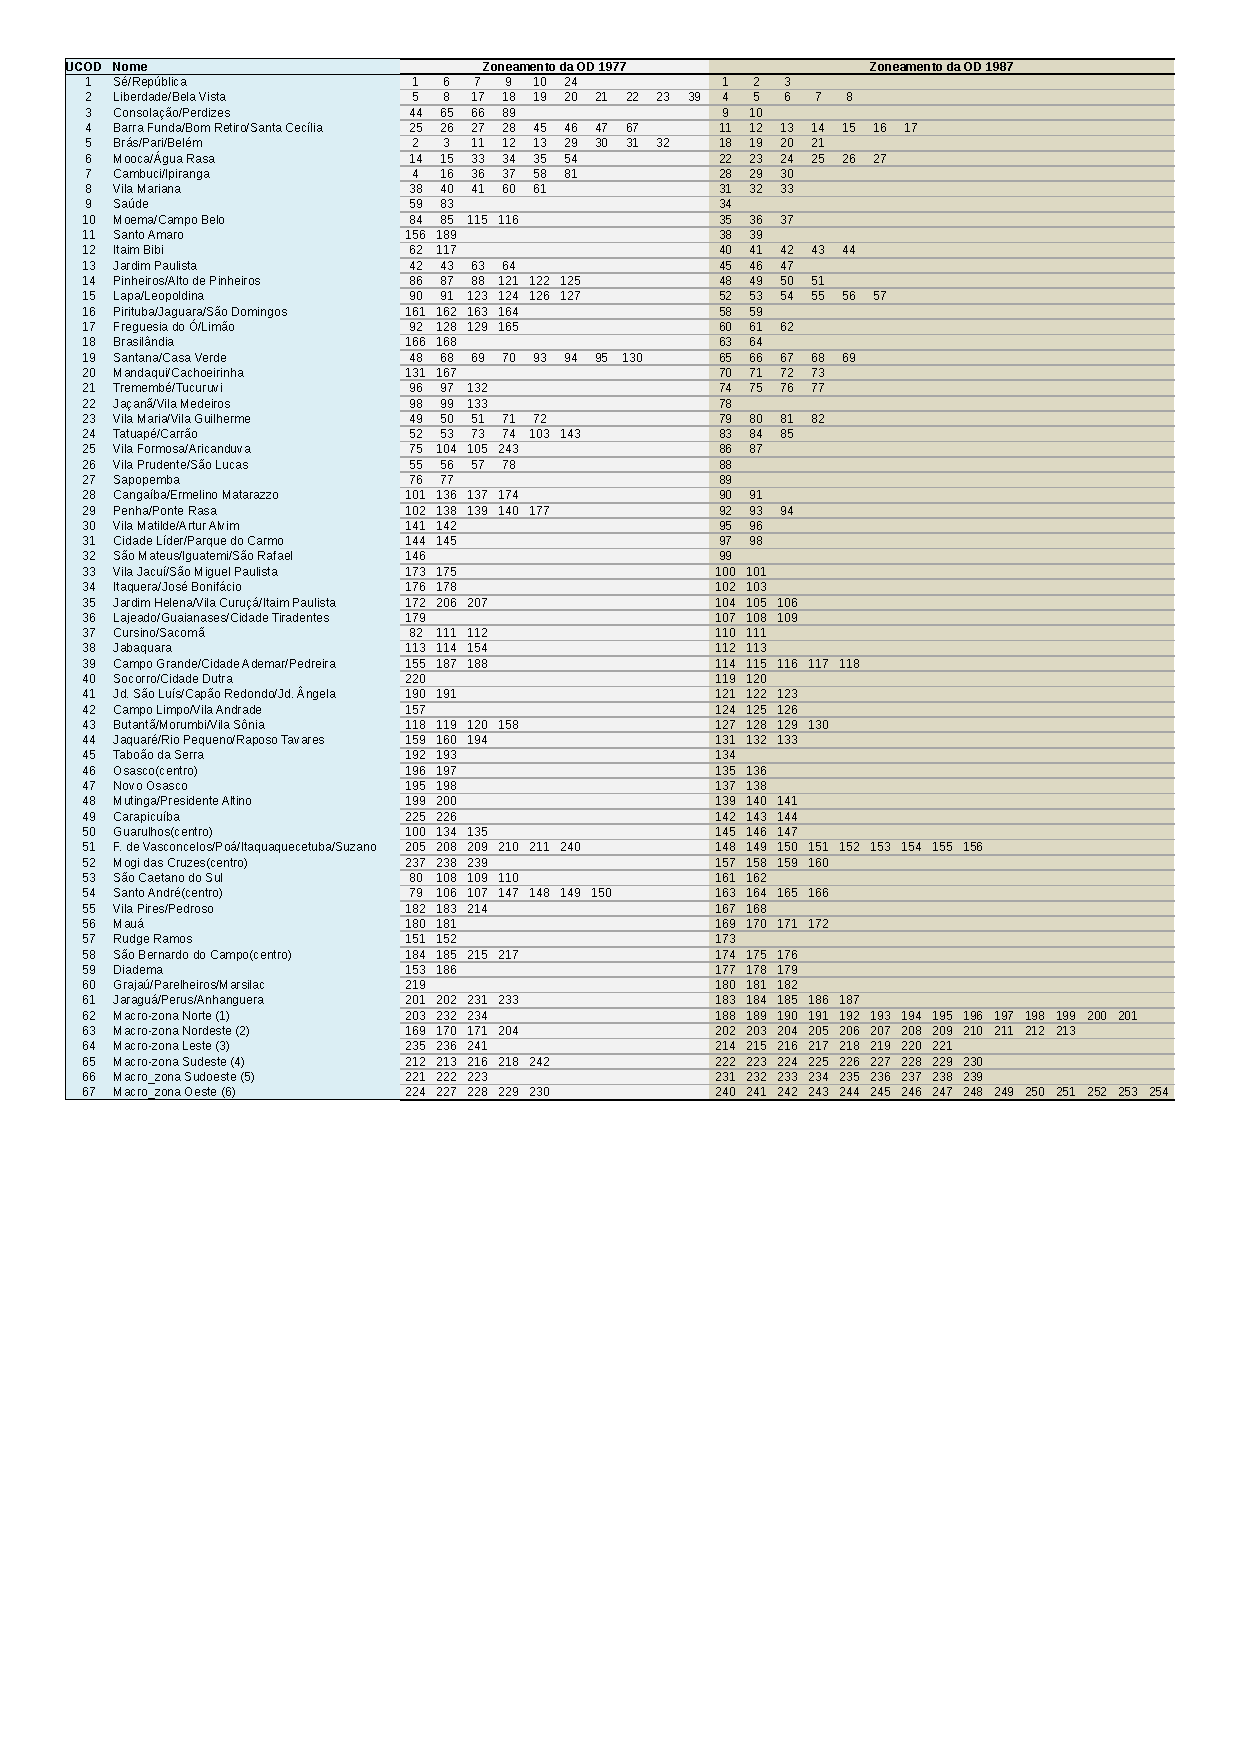
\includepdf{anexos/UCOD01.pdf}
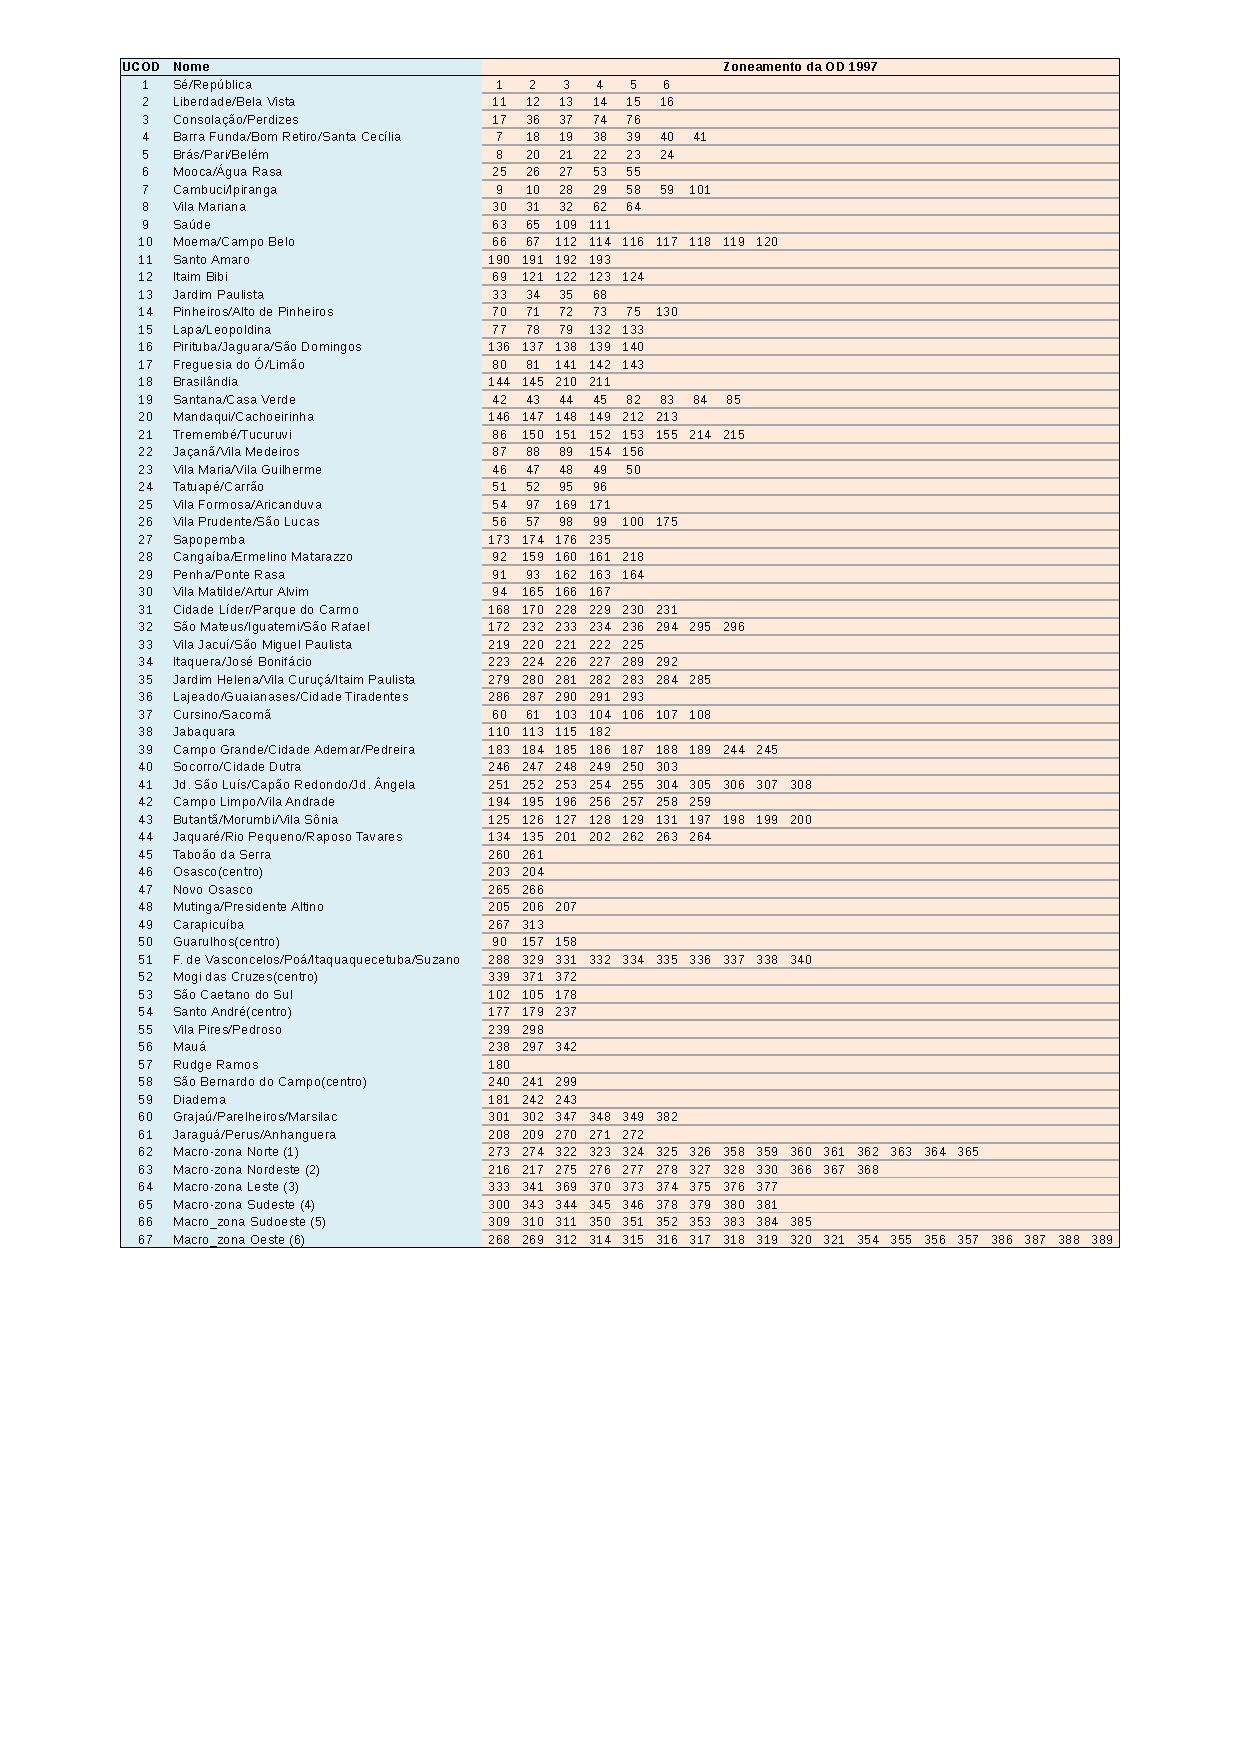
\includepdf{anexos/UCOD02.pdf}
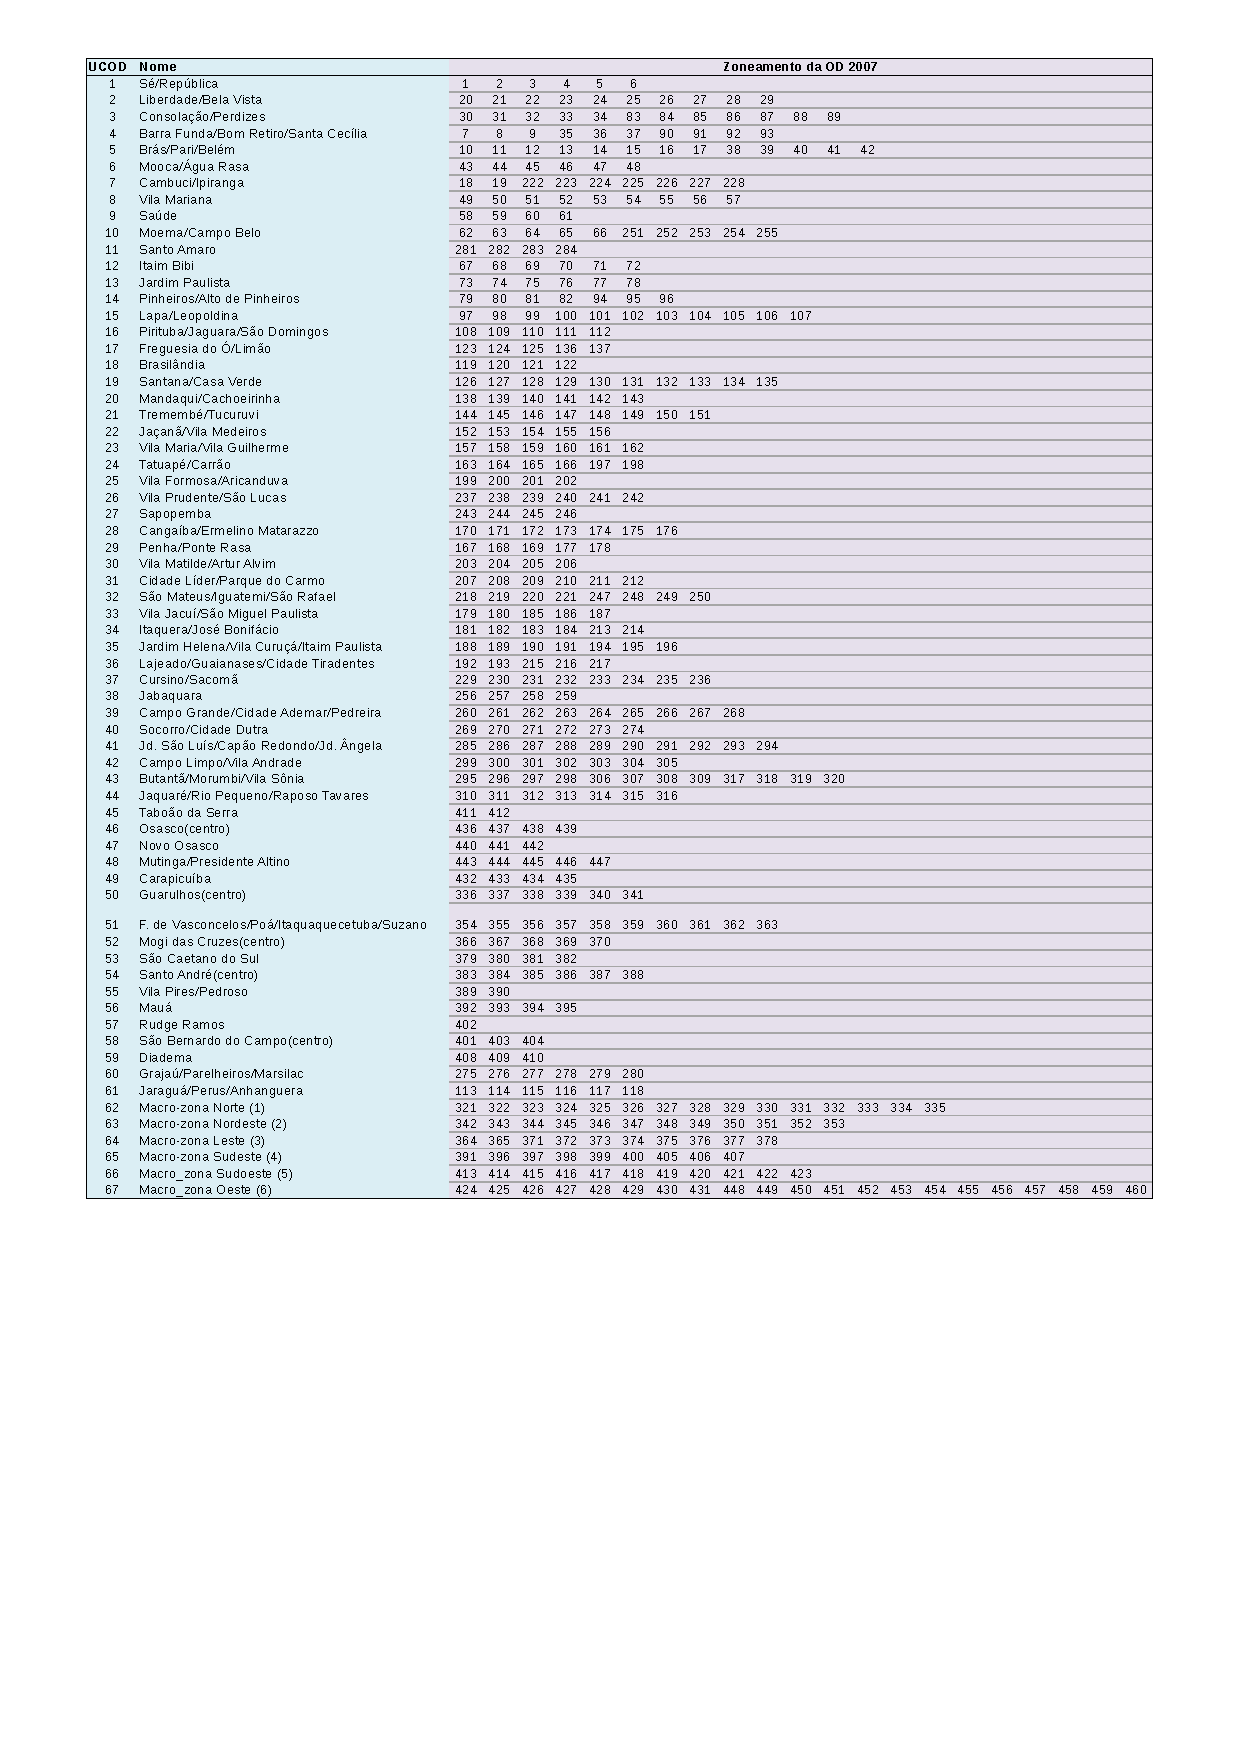
\includepdf{anexos/UCOD03.pdf}
%% ---
%%%%%%%%%%%%%%%%%%%%%%%%%%%%%%%%%%%%%%%%%%%
%% ---
\chapter{Layouts dos bancos de dados das Pesquisas Origem-Destino do Metrô-SP (1977, 1987, 1997 e 2007)}\label{chap:anexo_layouts}
%% ---
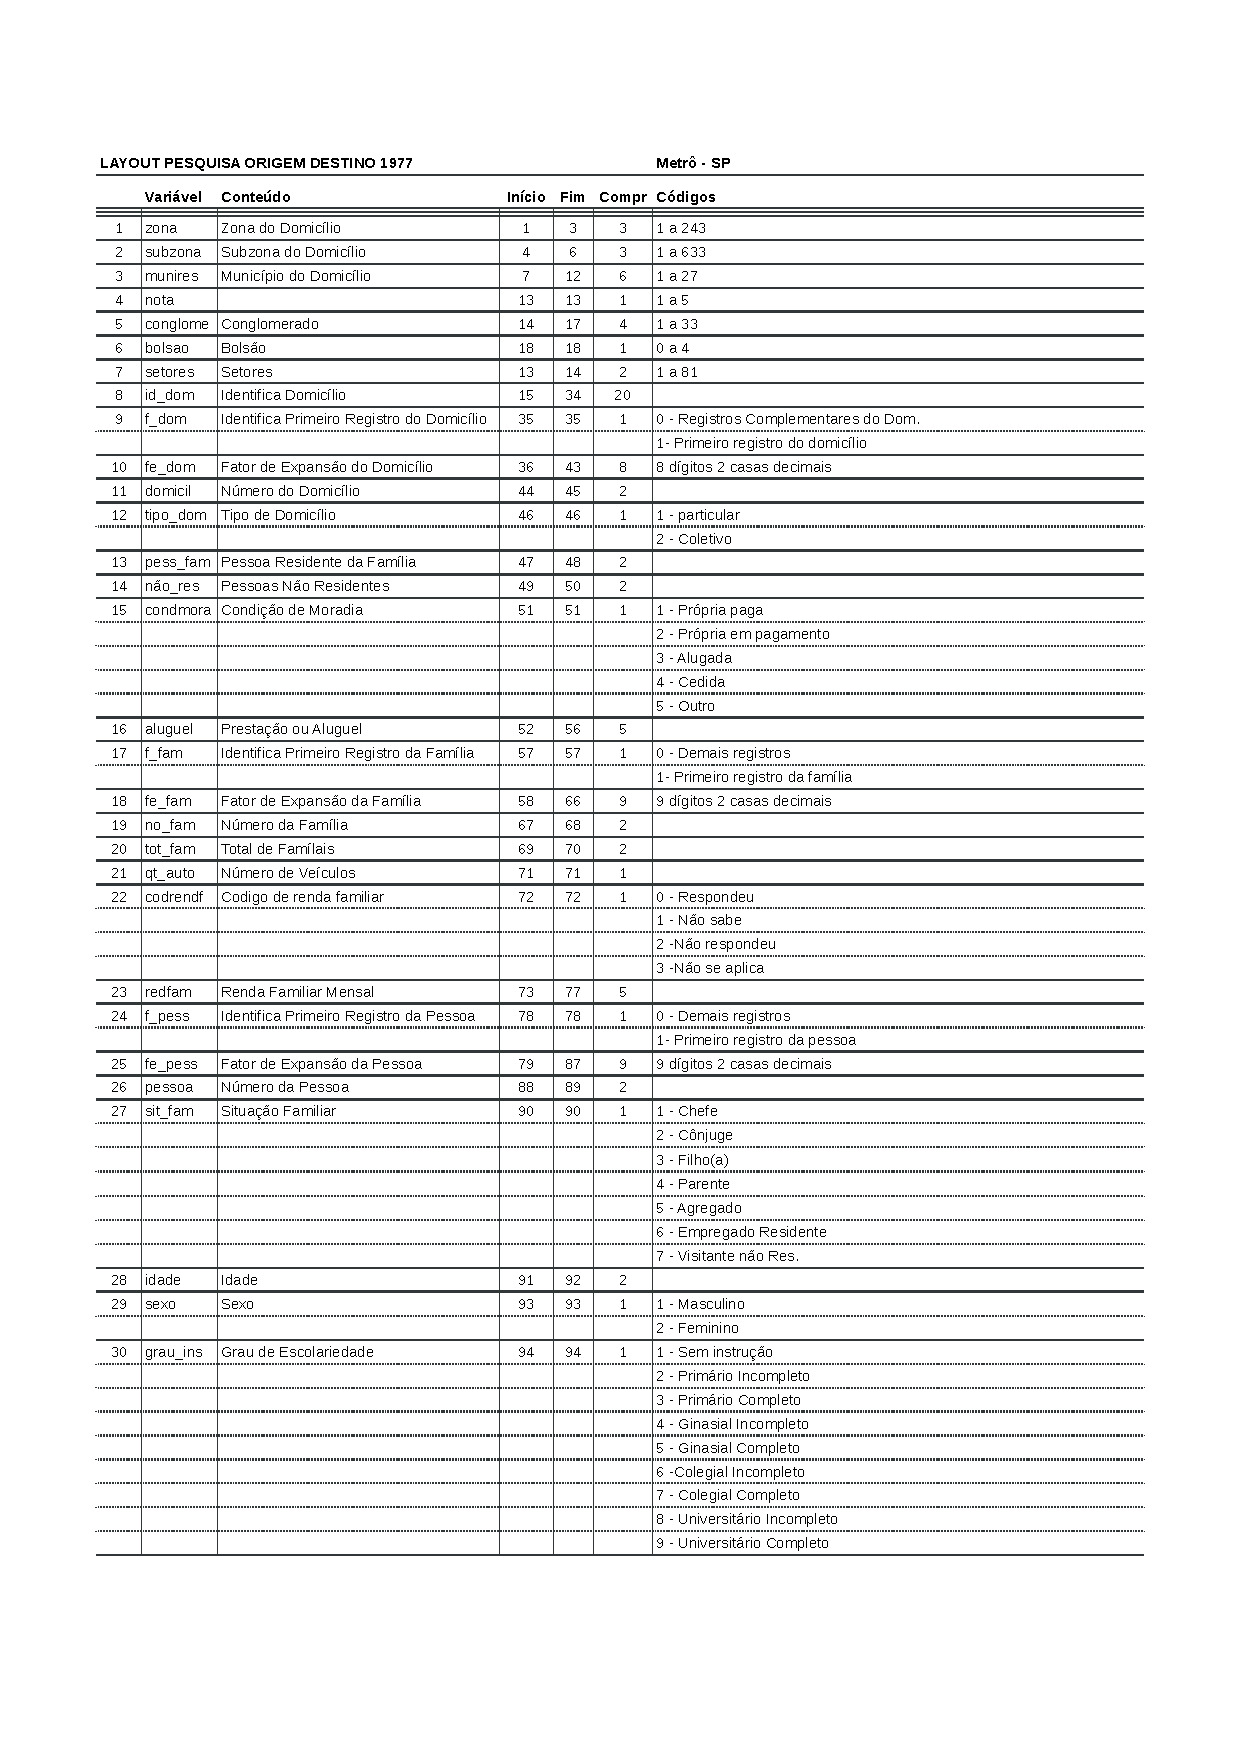
\includepdf[pages=-]{anexos/layout77.pdf}
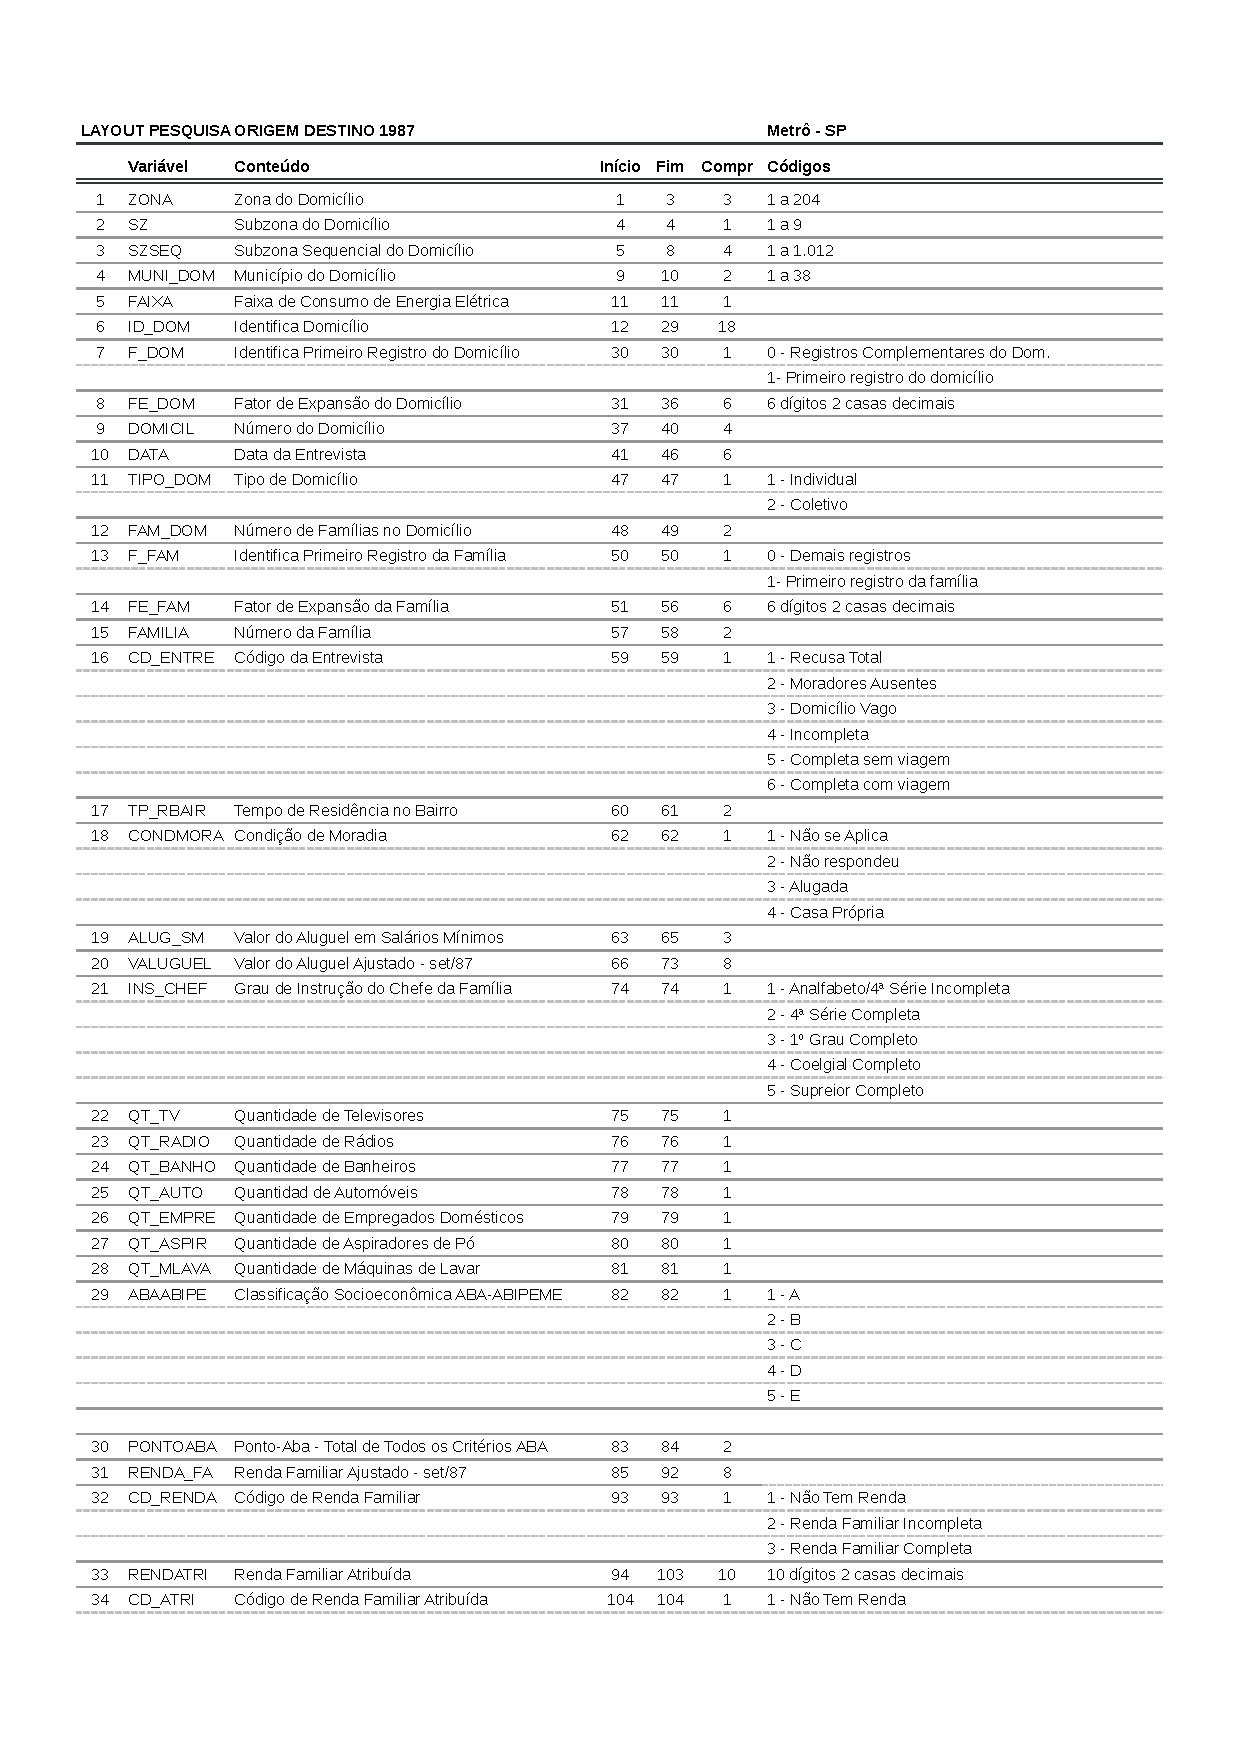
\includepdf[pages=-]{anexos/layout87.pdf}
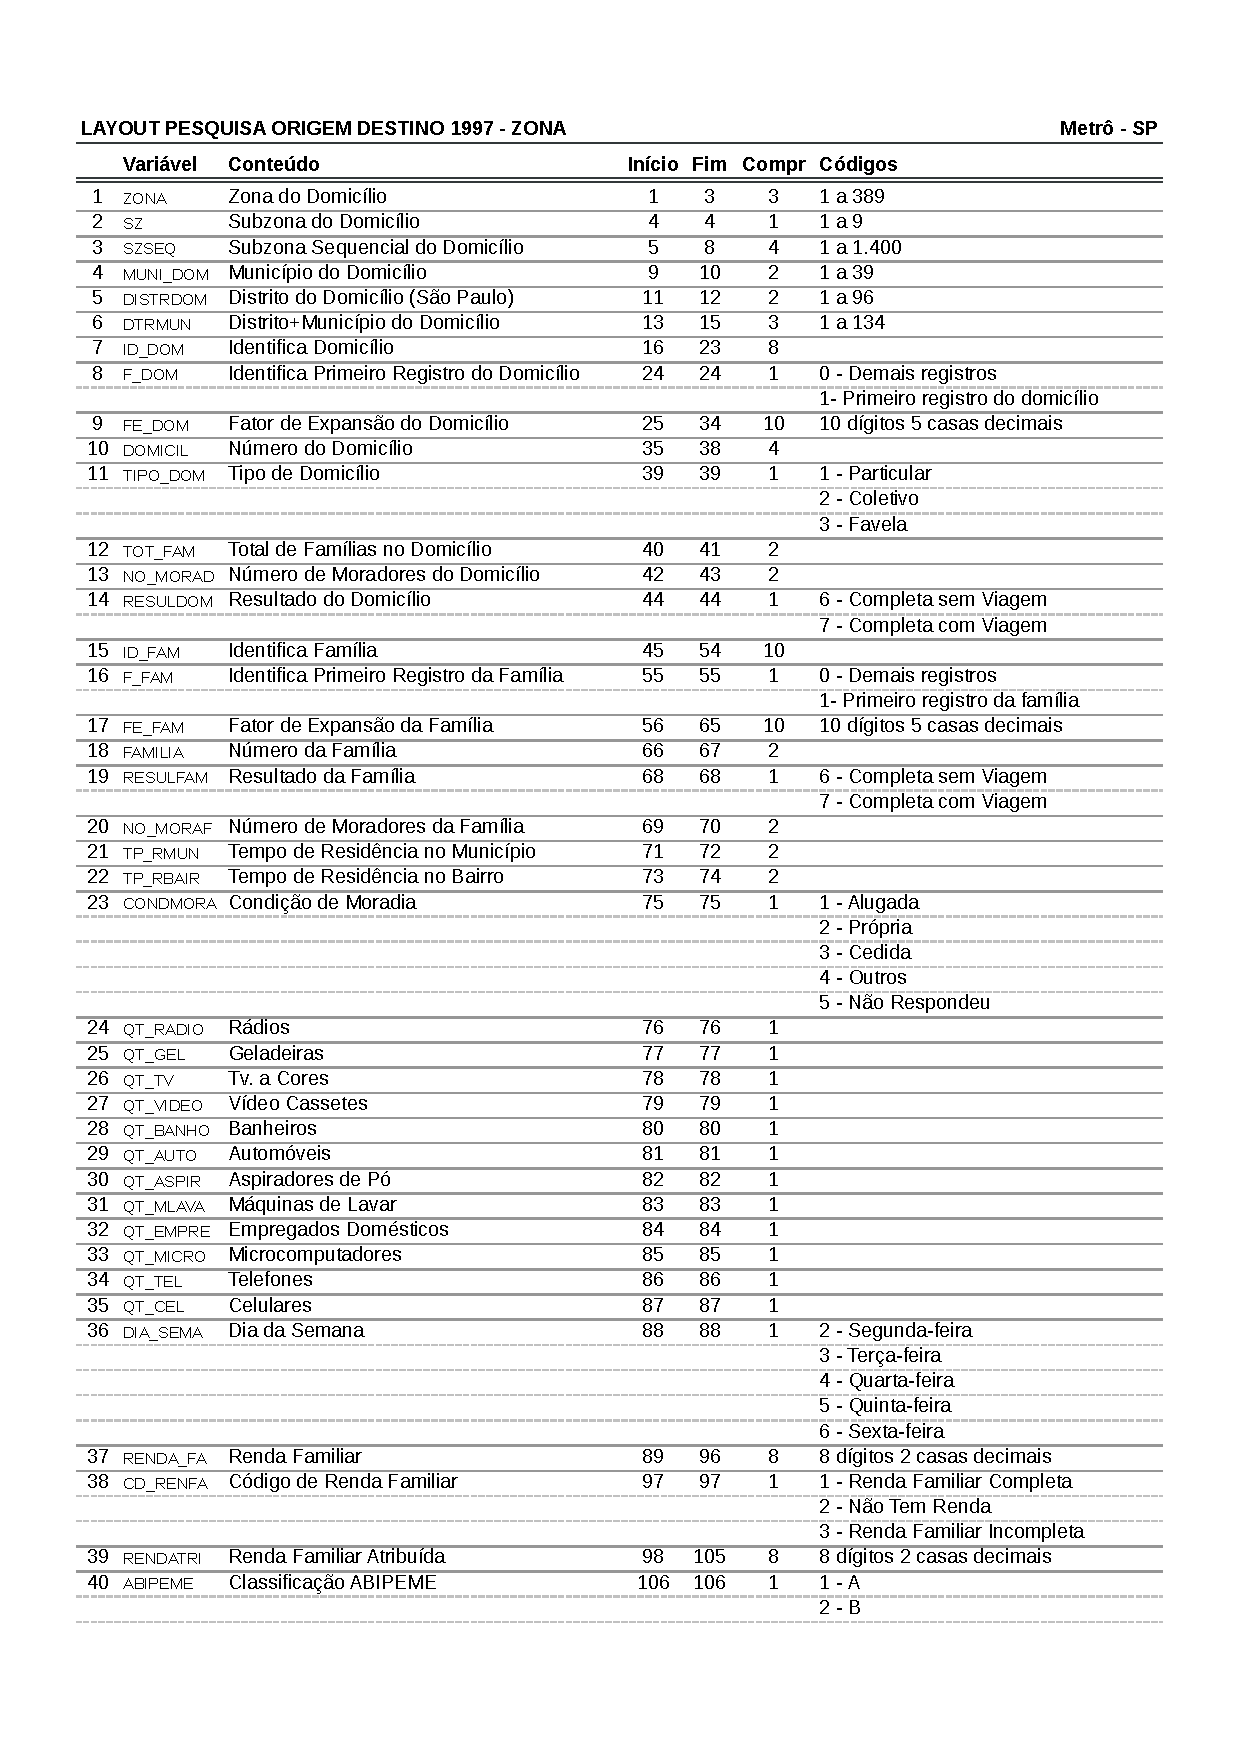
\includepdf[pages=-]{anexos/layout97.pdf}
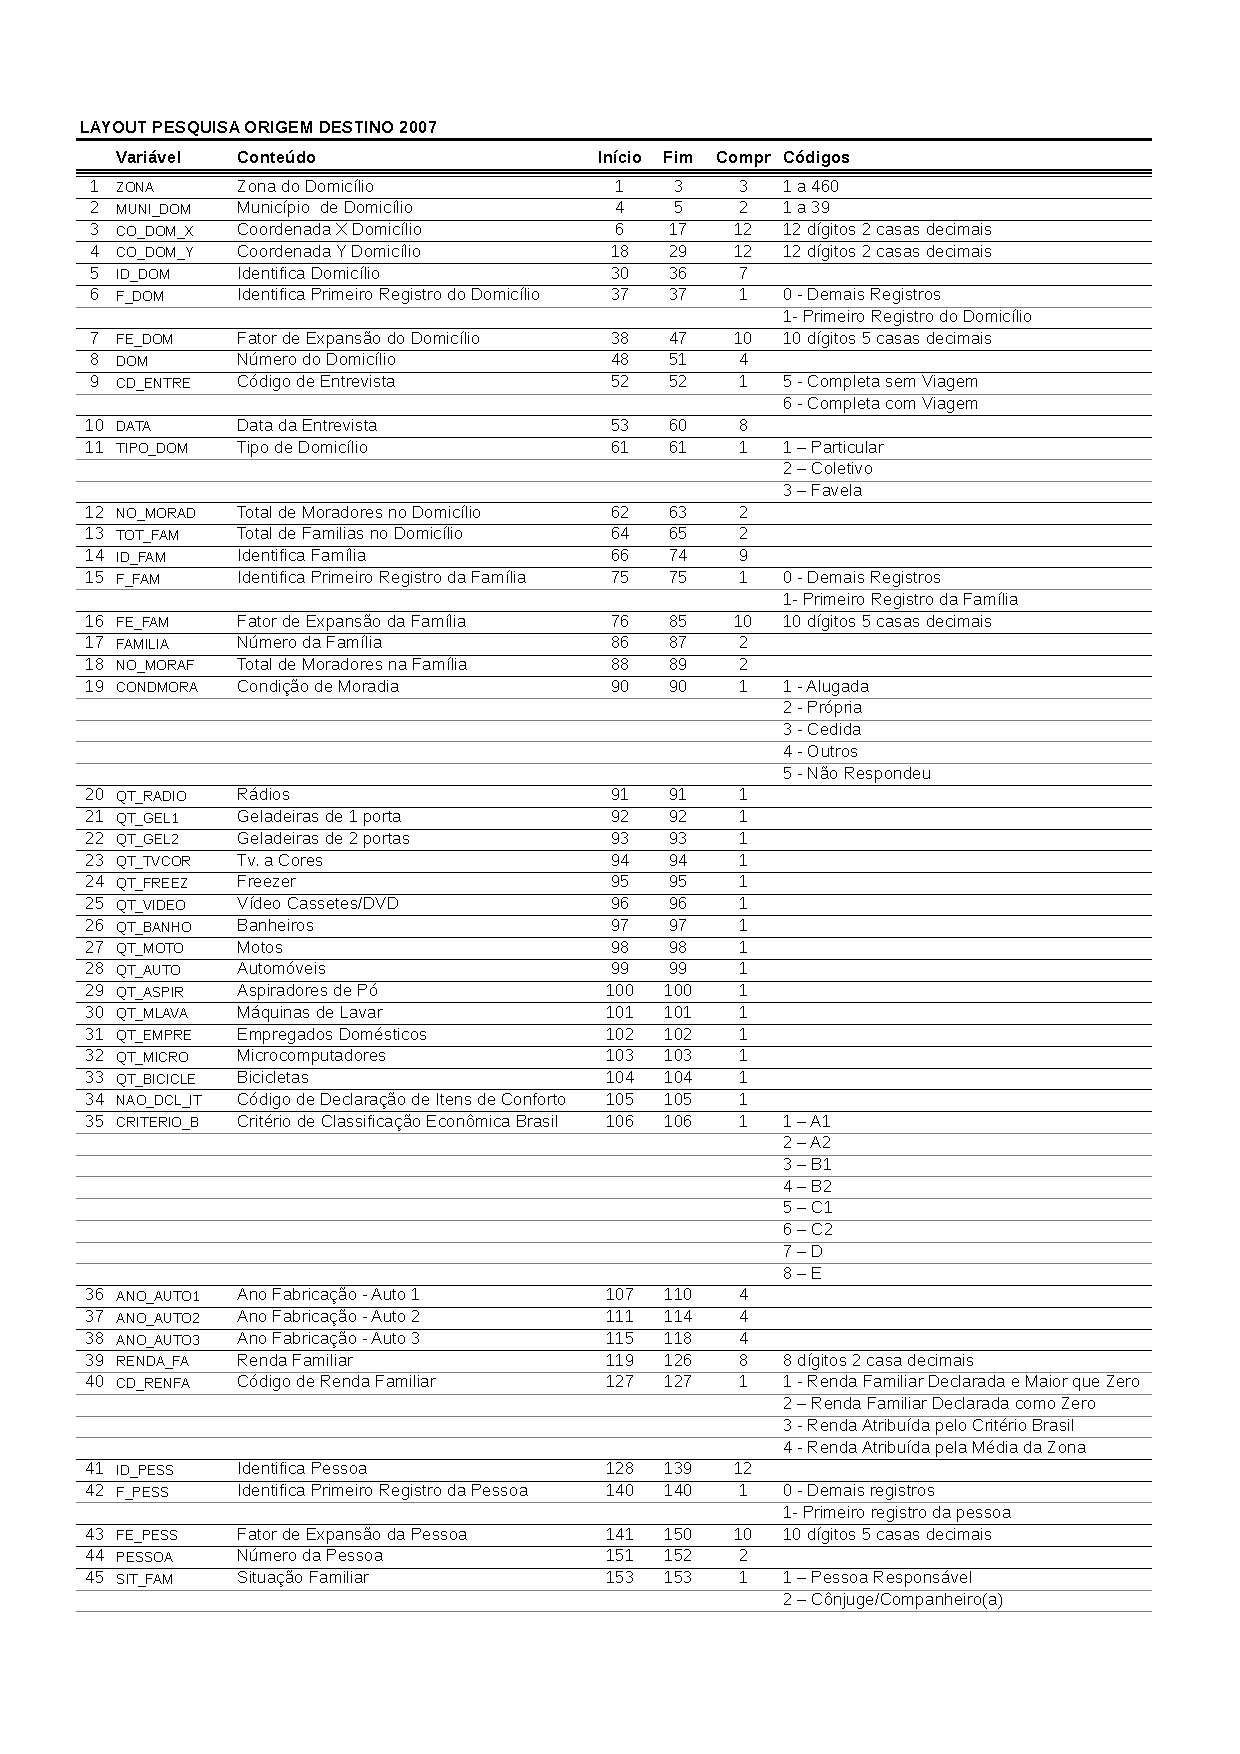
\includepdf[pages=-]{anexos/layout07.pdf}
%% ---
%\input{./anexos/questao-aberta-piloto}
%% ---




% ---
%% ---

\end{anexosenv}

%---------------------------------------------------------------------
% INDICE REMISSIVO
%---------------------------------------------------------------------
\phantompart
\printindex
%---------------------------------------------------------------------
%\listoftodos
\end{document}
